\documentclass[a4paper]{article}
\usepackage[paper=a4paper, left=1.5cm, right=1.5cm, bottom=1.5cm, top=3.5cm]{geometry}
\usepackage[spanish, es-noquoting, activeacute]{babel}
\usepackage[utf8]{inputenc}
\usepackage{amsthm}
\usepackage{amsmath}
\usepackage{amsfonts}
\usepackage{amssymb}
\usepackage{graphicx}
\usepackage{url}
\usepackage{verbatim}
\usepackage{color}
\usepackage{hyperref}

\usepackage[lined, ruled, linesnumbered]{algorithm2e}

\usepackage{footnote}
\usepackage{todonotes}

\parskip = 5pt
\parindent = 0pt

\newtheorem{teo}{Teorema}[section]
\newtheorem{propo}{Proposici\'{o}n}[section]
\newtheorem{propi}{Propiedad}[section]
\newtheorem{lema}{Lema}[section]
\newtheorem{coro}{Corolario}[section]

\theoremstyle{definition}
\newtheorem{defi}{Definici\'{o}n}[section]

\theoremstyle{definition}
\newtheorem{obs}{Observaci\'{o}n}[section]

\providecommand{\norm}[1]{\left\lVert#1\right\rVert}
\providecommand{\bold}[1]{{\boldsymbol #1}}

\newcommand{\tab}[0]{\hspace{2cm}}
\newcommand{\fdos}[4]{
	\left\{
		\begin{array}{lll}
			#1 & \mbox{si } #2 \\
			#3 & \mbox{si } #4
		\end{array}
	\right.
}

\newcommand{\ftres}[6]{
	\left\{
		\begin{array}{lll}
			#1 & \mbox{if } #2 \\
			#3 & \mbox{if } #4 \\
			#5 & \mbox{if } #6
		\end{array}
	\right.
}

\def\N{\mathbb{N}}
\def\R{\mathbb{R}}
\def\Z{\mathbb{Z}}
\def\Q{\mathbb{Q}}
\def\C{\mathbb{C}}
\def\S{\mathbb{S}}
\def\V{\mathbb{V}}
\def\W{\mathbb{W}}
\def\x{\times}
\newcommand{\rn}[2]{\in\R^{#1\x #2}}

\graphicspath{{imagenes/}}

\makesavenoteenv{tabular}

\begin{document}

\newpage
\setcounter{page}{1}
\pagenumbering{arabic}
\pagestyle{plain}

\hfill 
\includegraphics[scale = 0.75]{imagenes/logo_dc.jpg}~\\[0.25cm]

\begin{center}
	\textbf{\Large Notas de Métodos Numéricos}\\[1cm]
	{\large Guido Tagliavini Ponce\\[0.15cm]}
	Universidad de Buenos Aires\\[0.15cm]
	\texttt{guido.tag@gmail.com}\\[1cm]
	\textbf{v1.3 (\today)}\\[1cm]
\end{center}
\rule{\linewidth}{0.2mm}

\tableofcontents
\newpage
\section{Elementos de Álgebra Lineal}

Esta sección provee nociones básicas de Álgebra Lineal necesarias para el curso,
pero no se pretende profundizar demasiado, ya que no es una materia especifica de Álgebra Lineal.

\subsection{Espacio y Subespacio Vectorial}
\begin{defi}
	Un Espacio Vectorial $(V, +, \bullet , K)$ es una estructura algebraica creada sobre
	el conjunto no vacio $V$, con una operación interna llamada \textit{suma} definida
	para los elementos del conjunto $V$ y una operación externa llamada \textit{producto} definida
	entre los elementos del conjunto $V$ y el conjunto $K$, que debe tener estructura
	de cuerpo. Dicha estructura debe cumplir las siguientes 8 propiedades:
	\begin{enumerate}
		\item La \textit{suma} debe ser conmutativa, es decir: $ u + v = v + u \quad \forall\ u,v \in V$
		\item La \textit{suma} debe ser asociativa, es decir: $ u + (v + w) = (u + v) + w \quad \forall\ u,v,w \in V$
		\item La \textit{suma} debe tener elemento neutro, es decir: $\exists\ 0 \in V : u + 0 = u \quad \forall\ u \in V$
		\item La \textit{suma} debe tener elemento inverso, es decir: $\forall\ u \in V,\ \exists\ -u \in V : u + (-u) = 0$
		\item El \textit{producto} debe ser asociativo, es decir: $ a \cdot (b \cdot u) = (a \cdot b) \cdot u \quad \forall\ a,b \in K,\ \forall\ u \in V$
		\item El \textit{producto} debe tener elemento neutro, es decir: $\exists\ 1 \in K : 1 \cdot u = u \quad \forall\ u \in V$
		\item El \textit{producto} debe ser distributivo respecto la \textit{suma} de vectores, es decir: $ a \cdot (u + v) = a \cdot u + a \cdot v \quad \forall\ a \in K,\ \forall\ u,v \in V$
		\item El \textit{producto} debe ser distributivo respecto la \textit{suma} de escalares, es decir: $ (a + b) \cdot u = a \cdot u + b \cdot u \quad \forall\ a,b \in K,\ \forall\ u \in V$
	\end{enumerate}
\end{defi}

\begin{defi}
	Si $\V$ es un Espacio Vectorial y $\S \subset \V$, decimos que
	$\S$ es un Subespacio Vectorial de $\V$ si:
	\begin{itemize}
		\item $0 \in \S$ (o que $\S \neq \emptyset$).
		\item $u,v \in \S \implies u + v \in \S$
		\item $u \in \S,\ \lambda \in K \implies \lambda \cdot u \in \S$
	\end{itemize}
\end{defi}

De ahora en más vamos a suponer que el conjunto $V$ es, por ejemplo, $\R^{n}$ y el cuerpo $K$ es $\R$.

\subsection{Combinación e Independencia Lineal}
Sea $\V$ un Espacio Vectorial y sean $\{v_1, \dots, v_k\} \subset \V$.
\begin{defi}
	Decimos que $w \in \V$ es \textit{combinación lineal} de $\{v_1, \dots, v_k\}$ si
	$\exists \lambda_1, \dots, \lambda_k \in \R / w = \lambda_1 v_1 + \dots + \lambda_k v_k$
\end{defi}

\begin{defi}
	Decimos que $\{v_1, \dots, v_k\}$ es \textit{linealmente independiente} si
	la única combinación lineal de ellos igualada a $0 \in \V$ es la combinación
	lineal ``trivial'' (coeficientes nulos)
	$$\lambda_1 v_1 + \dots + \lambda_k v_k = 0 \implies \lambda_1 = \lambda_2 = \dots = \lambda_k = 0$$
\end{defi}

\subsection{Conjunto de Generadores de un Espacio Vectorial}
Sea $\V$ un Espacio Vectorial y sean $\{v_1, \dots, v_k\} \subset \V$.
\begin{defi}
Decimos que $\langle v_1, \dots, v_k \rangle$ es un \textit{conjunto generador}
y genera el conjunto de todas las combinaciones lineales de $\{v_1, \dots, v_k\}$, o lo que es lo mismo:
	$$\langle v_1, \dots, v_k \rangle = \{\lambda_1 v_1 + \dots + \lambda_k v_k / \lambda_1, \dots, \lambda_k \in \R \}$$
\end{defi}

\subsection{Base de un Espacio Vectorial}
Sea $\V$ un Espacio Vectorial y sean $\{v_1, \dots, v_k\} \subset \V$, un conjunto
de generadores linealmente independientes.
\begin{defi}
	Decimos que $\{v_1, \dots, v_k\}$ forman una \textit{Base} de $\V$ y todo
	elemento de $\V$ se puede escribir como combinación lineal de $v_1, \dots, v_k$.
\end{defi}

\subsection{Dimensión de un Espacio Vectorial}
Sea $\V$ un Espacio Vectorial y sean $\{v_1, \dots, v_k\} \subset \V$ una Base de $\V$.
\begin{defi}
	La \textit{dimensión} de $\V$ es la cantidad de vectores en la Base, es decir $k$,
	y se denota $dim(\V)$.
\end{defi}

\subsection{Matrices: definición y propiedades}
\begin{defi}
	Una \textbf{matriz} A de $m \x n$ es un arreglo de $m$ filas y $n$ columnas. \\
	\begin{center}
		$\begin{bmatrix}
			a_{1,1} & a_{1,2} & a_{1,3} & \cdots & a_{1,n} \\
			a_{2,1} & a_{2,2} & a_{2,3} & \cdots & a_{2,n} \\
			a_{3,1} & a_{3,2} & a_{3,3} & \cdots & a_{3,n} \\
			\vdots & \vdots & \vdots & \ddots & \vdots \\
			a_{m,1} & a_{m,2} & a_{m,3} & \cdots & a_{m,n}
		\end{bmatrix}$
	\end{center}
\end{defi}

\subsubsection{Rango}
El rango de una matriz es el número de filas (o columnas) linealmente independientes.

\subsubsection{Inversibilidad}
Sea $A \rn{n}{n}$. Se dice que $A$ es inversible sii $\exists\ B\rn{n}{n} / A\cdot B = B\cdot A = I$.

$B$ se nota como $A^{-1}$

\underline{Obs:}
\begin{itemize}
	\item Si $\exists A^{-1}$ entonces es única
\end{itemize}

\underline{Nomenclatura:} Si $A$ es inversible, se dice \textbf{no singular}. Si es \textbf{singular}, es no inversible.

\subsubsection{Determinante}
Sea $A \rn{m}{n}$. $det(A)\in\R$\\
\underline{Obs:}
\begin{itemize}
	\item $det(A\cdot B) = det(A) \cdot det(B)$
	\item $det(A^{-1}) = \displaystyle \frac{1}{det(A)}$
	\item $det(A)\neq 0 \Leftrightarrow \exists A^{-1}$
\end{itemize}

\subsubsection{Traza}
Sea $A \rn{m}{n}$.

\begin{defi}
	Definimos la \textit{traza} de $A$ como la suma de los elementos de la diagonal:
	$$tr(A) = \sum_{i=1}^{min(m,n)}{a_{ii}}$$
\end{defi}

\subsection{Operaciones sobre matrices}
Sobre las matrices se pueden aplicar las siguientes operaciones:

\subsubsection{Suma}
$A + B = C$ sii $A$ y $B$ tienen la misma dimesión (i.e., $A$,$B \in \R^{m\x n} \Rightarrow C \in R^{m\x n}$).
	\begin{center}
		$a_{i,j} + b_{i,j} = c_{i,j} \tab \forall i=1\cdots m \; \forall j = 1\cdots n$
	\end{center}

\subsubsection{Igualdad}
A=B sii $A$ y $B$ tienen la misma dimensión.
	\begin{center}
		$a_{i,j} = b_{i,j} \tab \forall i=1\cdots m \; \forall j = 1\cdots n$
	\end{center}

\subsubsection{Producto por escalar}
Sea $\lambda \in \R$. $\lambda \cdot A = B$ ($A\in\R^{m\x n} \Rightarrow B \in \R^{m\x n}$)
	\begin{center}
		$\lambda \cdot a_{i,j} = b_{i,j}\tab \forall i = 1 \cdots m , j = 1 \cdots n$
	\end{center}

\subsubsection{Producto} $A\cdot B = C$ sii $A\in\R^{m\x n}$ y $B\in\R^{n\x p} \Rightarrow C\in\R^{m\x p}$
	\begin{center}
		$c_{i,j} = \displaystyle \sum_{k=1}^n a_{i,k}\cdot b_{k,j}$
	\end{center}
	Observar que no necesariamente vale que $AxB = BxA$.

\subsubsection{Inversa}
Sea $A\in\R^{n\x n}$ inversible y $B\in\R^{n\x n}$ dicha matriz inversa, entonces:
$A^{-1} = B$

\underline{Obs:}
\begin{itemize}
	\item $(A^{-1})^{-1} = A$
	\item Sean $A$ y $B \in \R^{n\x n}$ inversibles. Entonces $(A\cdot B)^{-1} = B^{-1} \cdot A^{-1}$
\end{itemize}

\subsubsection{Transpuesta}
	Sea $A\rn{m}{n}$. Se define $A^t\rn{n}{m}$ como
	\begin{center}
		$(A^t)_{i,j} = A_{j,i} \tab \forall i=1\cdots n,j=1\cdots m$
	\end{center}

	\underline{Obs:}
	\begin{itemize}
		\item $(A+B)^t = A^t+B^t$
		\item $(A\cdot B)^t = B^t\cdot A^t$
		\item $(A^{-1})^t = (A^t)^{-1}$
	\end{itemize}


\subsection{Matrices Elementales}

\subsubsection{Identidad} $I$ matriz identidad. $I \in R^{n\x n}$
	\begin{center}$I_{i,j} =
		\fdos
		{1}	{i=j}
		{0}	{i\neq j} \tab \forall i,j=1\cdots n$
	\end{center}
	Consecuentemente, la forma de la matriz identidad de $\R^{n\x n}$ es:
	\begin{center}
		$\begin{bmatrix}
			1 & 0 & 0 & \cdots & 0 \\
			0 & 1 & 0 & \cdots & 0 \\
			0 & 0 & 1 & \cdots & 0 \\
			\vdots & \vdots & \vdots & \ddots & \vdots \\
			0 & 0 & 0 & \cdots & 1
		\end{bmatrix}$
	\end{center}

\underline{Obs:} $I \cdot A = A \cdot I = A \tab \forall A\in\R^{n\x n}$

\subsubsection{Matrices de permutación}
Una matriz de permutación $P$ es una matriz que permite permutar filas o columnas de una matriz $A$ al realizar:
\begin{itemize}
	\item $P \cdot A$ permuta las filas de $A$
	\item $A \cdot P$ permuta las columnas de $A$
\end{itemize}

La matriz $P$ se obtiene permutando las columnas de la matriz identidad $(I)$. Observemos en un ejemplo de $3 \x 3$ en el que llamamos $1$, $2$ y $3$ a las columnas de la matriz identidad de la siguiente forma:
\begin{center}
	$I = \begin{bmatrix}
		1&0&0\\
		0&1&0\\
		0&0&1
	\end{bmatrix} = (1,2,3)$
\end{center}

Si permutamos, por ejemplo, las filas $1$ y $2$, obtenemos la siguiente matriz de permutación $P$:
\begin{center}
	$P=\begin{bmatrix}
		0&1&0\\
		1&0&0\\
		0&0&1
	\end{bmatrix} = (2,1,3)$
\end{center}

Si multiplicamos a izquierda esta matriz con cualquier otra, el resultado será esa misma matriz pero con la primer y segunda fila cambiadas de lugar (pues obtuvimos $P$ permutando la primer y segunda columnas de la identidad).

~\newline

\underline{Obs:} esta notación con índices permite almacenar una matriz de permutación $P\rn{n}{n}$ en sólamente $n$ elementos, en lugar de en los $n^2$ que normalmente tomaría.

\subsubsection{Triangular}
Una matriz es Triangular si los elementos por debajo o por arriba de la diagonal principal son cero.

En el primer caso, decimos que es Triangular Superior:

\begin{equation*}
	U =
	\left [ \begin{array}{ccccccc}
	  u_{11} & u_{12} & u_{13} & . & . & .& u_{1n}\\
	  0 & u_{22} & u_{23} & . & . & .& u_{2n}\\
	  0 & 0 & u_{33} & . & . & .& u_{3n}\\
	. & . & .. & . & . & .& .\\
	. & . & . & . & . & .& .\\
	. & . & . & . & . & .& .\\
	0 & 0 & 0 & . & . & .& u_{nn}\\
	\end{array} \right ]
\end{equation*}

Análogamente, en el segundo caso decimos que es Triangular Inferior:

\begin{equation*}
	L =
	\left [ \begin{array}{ccccccc}
	  l_{11} & 0 & 0 & . & . & .& 0\\
	  l_{21} & l_{22} & 0 & . & . & .& 0\\
	  l_{31} & l_{32} & l_{33} & . & . & .& 0\\
	. & . & . & . & . & .& .\\
	. & . & . & . & . & .& .\\
	. & . & . & . & . & .& .\\
	l_{n1} & l_{n2} & l_{n3} & . & . & .& l_{nn}\\
	\end{array} \right ]
\end{equation*}

\subsubsection{Diagonal}
Una matriz es Diagonal cuando los únicos elementos distintos de cero son los elementos
de la diagonal principal:
\begin{equation*}
	D =
	\left [ \begin{array}{ccccccc}
	  d_{11} & 0 & 0 & . & . & .& 0\\
	  0 & d_{22} & 0 & . & . & .& 0\\
	  0 & 0 & d_{33} & . & . & .& 0\\
	  . & . & . & . & . & .& .\\
	  . & . & . & . & . & .& .\\
	  . & . & . & . & . & .& .\\
	  0 & 0 & 0 & . & . & .& d_{nn}\\
	\end{array} \right ]
\end{equation*}

\underline{Obs:} dicha matriz es a la vez Triangular Superior e Inferior.

\subsubsection{Otras}
\subsubsection{(????)}

Una matriz de (????) $E$ es una matriz que permite multiplicar toda una fila o columna de una matriz $A$ por un escalar dado, al realizar:
\begin{itemize}
	\item $E\cdot A$ multiplica una fila de $A$ por un escalar $\lambda$.
	\item $A\cdot E$ multiplica una columna de $A$ por un escalar $\lambda$.
\end{itemize}

Dado el escalar $\lambda$, definimos la matriz $E$ de la forma:
\begin{center}
	$E=\begin{bmatrix}
		1 & \cdots & 0 & \cdots & 0 \\
		\vdots  & \ddots &   &        & \vdots  \\
		0 & \cdots & \lambda & \cdots & 0\\
		\vdots & & &\ddots & \vdots \\
		0&\cdots & 0 & \cdots & 1
	\end{bmatrix} \tab$ con $\lambda\in\R$
\end{center}


Si $\lambda$ está en la fila $s$ de la matriz $E$, entonces la fila $s$ de la matriz $B = E \cdot A$ es la fila $s$ de la matriz $A$ multiplicada por $\lambda$. Las restantes filas quedan iguales.

Ejemplos en $4\x 4$:
\begin{center}
	$\begin{bmatrix}
		1&0&0&0 \\
		0&1&0&0 \\
		0&0&\lambda&0 \\
		0&0&0&1
	\end{bmatrix} \cdot
	\begin{bmatrix}
		1&5&9&13 \\
		2&6&10&14 \\
		3&7&11&15 \\
		4&8&12&16
	\end{bmatrix} =
	\begin{bmatrix}
		1&5&9&13 \\
		2&6&10&14 \\
		3\cdot\lambda&7\cdot\lambda&11\cdot\lambda&15\cdot\lambda \\
		4&8&12&16
	\end{bmatrix}
	$
\end{center}

\begin{center}
	$\begin{bmatrix}
		1&5&9&13 \\
		2&6&10&14 \\
		3&7&11&15 \\
		4&8&12&16
	\end{bmatrix} \cdot
	\begin{bmatrix}
			1&0&0&0 \\
			0&1&0&0 \\
			0&0&\lambda&0 \\
			0&0&0&1
		\end{bmatrix} =
	\begin{bmatrix}
		1&5&9\cdot\lambda&13 \\
		2&6&10\cdot\lambda&14 \\
		3&7&11\cdot\lambda&15 \\
		4&8&12\cdot\lambda&16
	\end{bmatrix}
	$
\end{center}


\subsubsection{(????)}
Una matriz de (????) $E$ es una matriz que permite sumar dos filas o columnas de una matriz $A$, multiplicando una de ellas por un escalar dado.

Dado el escalar $\lambda$, se define $E$ como:
\begin{center}
	$E = \begin{bmatrix}
		1 & & & & \\
		& \ddots & & & \\
		& & 1 & & \\
		& & \lambda & \ddots & \\
		& & & & 1
	\end{bmatrix}$
\end{center}

(Observar que es la matriz identidad con $\lambda$ en algún lugar de algún $0$).

Suponiendo que $\lambda$ está en la fila $i$ y columna $j$, vale que
\begin{itemize}
	\item $E \x A$ multiplica la $j$-ésima fila de $A$ por $\lambda$ y se la suma a la $i$-ésima fila de $A$.
	\item $A \x E$ multiplica la $j$-ésima columna de $A$ por $\lambda$ y se la suma a la $i$-ésima columna de $A$.
\end{itemize}

\underline{Ejemplo:}
\begin{center}
	$\begin{bmatrix}
		1&0&0\\
		0&1&0\\
		0&\lambda&1
	\end{bmatrix}\x
	\begin{bmatrix}
		1&4&-7\\
		2&5&8\\
		3&6&9
	\end{bmatrix} =
	\begin{bmatrix}
		1&4&7\\
		2&5&8\\
		2\cdot\lambda+3 & 5\cdot\lambda + 6 & 8\cdot\lambda +9
	\end{bmatrix}$
\end{center}

\subsection{Transformaciones lineales}
Sean $\V$, $\W$ dos Espacios Vectoriales con cuerpo en $\R$
\begin{defi}
	Una función $f: \V \to \W$ se llama \textit{trasnformación lineal} si respeta
	las operaciones:
	\begin{itemize}
		\item $f(u + v) = f(u) + f(v) \quad \forall u,v \in \V$
		\item $f(\lambda \cdot u) = \lambda \cdot f(u) \quad \forall u \in \V,\ \forall \lambda \in \R$
	\end{itemize}
\end{defi}

\begin{teo}
	Si $f: \V \to \W$ es una transformación lineal $\implies f(0) = 0$
\end{teo}

\begin{teo}
	Si $A \rn{m}{n}$ y definimos $f: \R^{n} \to \R^{m}$ con la forma $f(x) = Ax$.

	Entonces, $f$ es una transformación lineal y lo llamamos transformación lineal
	asociada a $A$.
\end{teo}

\begin{propi}
	Si $f$ es transformación lineal asociada a una matriz $A$, entonces
	\begin{center}
		$A$ es inversible $\iff$ $f$ es biyectiva
	\end{center}
	\underline{Obs:} La matriz asociada a $f^{-1}$ es $A^{-1}$.
\end{propi}

\subsection{Imagen y Nucleo}
Sea $f: \V \to \W$ una transformación lineal y $A \rn{m}{n}$. Entonces,

\begin{defi} Definimos el \textit{Nucleo} (Nu) como
	\begin{itemize}
		\item $Nu(f) = \{v \in \V : f(v) = 0\}$ subespacio de $\V$
		\item $Nu(A) = \{x \in \R^{n} : Ax = 0 \in \R^{m}\}$ subespacio de $\R^{n}$
	\end{itemize}
\end{defi}

\begin{defi} Definimos la \textit{Imagen} (Im) como
	\begin{itemize}
		\item $Im(f) = \{f(v) /\ v \in \V\}$ subespacio de $\W$
		\item $Im(A) = \{Ax /\ x \in \R^{n}\}$ subespacio de $\R^{m}$
	\end{itemize}
\end{defi}

\underline{Obs:} $Im(A)$ es igual al espacio generado por las columnas de $A$.

\subsection{Teorema de la Dimensión}
\begin{teo} Sea $A \rn{m}{n}$, y su transformación lineal asociada $f: \R^{n} \to \R^{m}$. Entonces,
	$$dim(Nu(A)) + dim(Im(A)) = dim(\R^{n}) = n$$
\end{teo}

\underline{Obs:} $dim(Im(A))$ es igual al rango columna de $A$, que a su vez es
igual a la cantidad de columnas linealmente independientes de $A$ (rango columna) y la cantidad de
filas linealmente independientes de $A$ (rango fila).

\subsection{Ortogonalidad}

\subsection{Normas: definición y propiedades}

\subsection{Diagonalización y Autovalores}

\newpage
\section{Normas}

\subsection{Definiciones}

\begin{defi}
Una función $f : \mathbb{R}^n \to \mathbb{R}$ es una norma vectorial si cumple:
\begin{enumerate}
\item $f(x) > 0$ para todo $x \neq 0$ y $f(0) = 0$.
\item $f(\lambda x) = |\lambda| f(x)$.
\item $f(x + y) \leq f(x) + f(y)$.
\end{enumerate}
\end{defi}

Algunos ejemplos de normas vectoriales son:
\begin{itemize}
\item $\norm{x}_1 = \sum_{i = 1}^{n} |x_i|$
\item $\norm{x}_2 = \left(\sum_{i = 1}^{n} x_i^2\right)^{1/2}$
\item $\norm{x}_{\infty} = \max\limits_{1 \leq i \leq n}|x_i|$
\end{itemize}

El concepto se extiende naturalmente para matrices.

\begin{defi}
Una función $F : \mathbb{R}^{n \times n} \to \mathbb{R}$ es una norma matricial si cumple:
\begin{enumerate}
\item $F(A) > 0$ para toda $A \neq 0$ y $F(0) = 0$.
\item $F(\lambda A) = |\lambda| F(A)$.
\item $F(A + B) \leq F(A) + F(B)$.
\end{enumerate}
\end{defi}

Un ejemplo de norma matricial es la norma de Frobenius, una extensión aparentemente natural de la norma 2:
\begin{itemize}
\item $\norm{A}_F = \left(\sum_{i = 1}^{n} \sum_{j = 1}^{n} A_{ij}^2\right)^{1/2}$
\end{itemize}

Una propiedad no necesaria, aunque deseable, es la de submultiplicatividad.

\begin{defi}
Si $F : \mathbb{R}^{n \times n} \to \mathbb{R}$ es una norma matricial, $F$ se dice submultiplicativa si

\[F(AB) \leq F(A)F(B)\]

para todas $A, B \in \mathbb{R}^{n \times n}$.
\end{defi}

Otra propiedad notable de las normas es la de consistencia.

\begin{defi}
Si $F : \mathbb{R}^{n \times n} \to \mathbb{R}$ es una norma matricial y $f : \mathbb{R}^n \to \mathbb{R}$ es una norma vectorial, $F$ se dice consistente con $f$ si 

\[f(Ax) \leq F(A)f(x)\]

para todos $A \in \mathbb{R}^{n \times n}$, $x \in \mathbb{R}^n$.
\end{defi}

\subsection{Normas inducidas}

\begin{defi}
Sea $f : \mathbb{R}^n \to \mathbb{R}$ una norma vectorial. Definimos $F : \mathbb{R}^{n \times n} \to \mathbb{R}$ como

\[
F(A) = \max\limits_{x : f(x) = 1} f(Ax)
\]

$F$ resulta una norma matricial y se la llama norma inducida por $f$.
\end{defi}

A partir de ahora simbolizaremos tanto las normas vectoriales como sus respectivas normas matriciales inducidas mediante $\norm{\cdot}$, y el significado quedará claro por el contexto.

Las normas inducidas son de especial interés por lo siguiente.

\begin{propo}
Si $\norm{\cdot} : \mathbb{R}^{n \times n} \to \mathbb{R}$ es una norma matricial inducida, entonces $\norm{\cdot}$ es submultiplicativa y consistente, es decir que
\begin{enumerate}
\item $\norm{AB} \leq \norm{A}\norm{B}$
\item $\norm{Ax} \leq \norm{A}\norm{x}$
\end{enumerate}

\begin{proof}
\begin{enumerate}
\item Sea $x_0 \in \mathbb{R}^n$ unitario, que realiza la norma de $AB$. Entonces

\[\norm{AB} = \norm{ABx_0} = \norm{A\frac{Bx_0}{\norm{Bx_0}}}\norm{Bx_0}\]

Como $\frac{Bx_0}{\norm{Bx_0}}$ es un vector unitario, entonces $\norm{A\frac{Bx_0}{\norm{Bx_0}}} \leq \norm{A}$. Análogamente, $\norm{Bx_0} \leq \norm{B}$. Finalmente, como todos los factores son positivos, $\norm{AB} \leq \norm{A} \norm{B}$.

\item Sea $x \in \mathbb{R}^n$ cualquiera. Entonces $\norm{A} \geq \norm{A \frac{x}{\norm{x}}} = \frac{\norm{Ax}}{\norm{x}}$ pues $\frac{x}{\norm{x}}$ es unitario. Luego $\norm{Ax} \leq \norm{A}\norm{x}$.
\end{enumerate}
\end{proof}
\end{propo}

\subsection{Normas matriciales clásicas}

\begin{propo}
Sea $A \in \mathbb{R}^{n \times n}$. Entonces

\[\norm{A}_{1} = \max\limits_{1 \leq j \leq n} \norm{col_j(A)}_1\]

\begin{proof}
($\geq$) Sea $1 \leq j \leq n$ arbitrario, entonces

\[\norm{A}_1 = \max\limits_{x : \norm{x}_1 = 1} \norm{Ax}_1 \geq \norm{A e_j}_1 = \norm{col_j(A)}_1\]

Como $j$ es cualquiera, resulta que $\norm{A}_1 \geq \max\limits_{1 \leq j \leq n} \norm{col_j(A)}_1$.\\[0.25cm]

($\leq$)

\begin{align*}
\norm{A}_1 &= \max\limits_{x : \norm{x}_1 = 1} \norm{Ax}_1\\
& = \max\limits_{x : \norm{x}_1 = 1} \norm{(fil_1(A) x, \cdots, fil_n(A) x)}_1\\
& = \max\limits_{x : \norm{x}_1 = 1} \sum_{i = 1}^n |fil_i(A) x|\\
& = \max\limits_{x : \norm{x}_1 = 1} \sum_{i = 1}^n \left|\sum_{j = 1}^n a_{ij} x_j\right|\\
& \leq \max\limits_{x : \norm{x}_1 = 1} \sum_{i = 1}^n \sum_{j = 1}^n |a_{ij}| |x_j|\\
& = \max\limits_{x : \norm{x}_1 = 1} \sum_{j = 1}^n |x_j| \left(\sum_{i = 1}^n |a_{ij}|\right)\\
& \leq \max\limits_{x : \norm{x}_1 = 1} \sum_{j = 1}^n |x_j| \left(\max\limits_{1 \leq k \leq n} \sum_{i = 1}^n |a_{ik}|\right)\\
& = \max\limits_{x : \norm{x}_1 = 1} \left(\max\limits_{1 \leq k \leq n} \sum_{i = 1}^n |a_{ik}|\right)\left(\sum_{j = 1}^n |x_j|\right)\\
& = \max\limits_{x : \norm{x}_1 = 1} \left(\max\limits_{1 \leq k \leq n} \norm{col_k(A)}_1\right) \norm{x}_1\\
& = \max \limits_{1 \leq j \leq n}\norm{col_j(A)}_1 
\end{align*}

\end{proof}
\end{propo}

\begin{propo}
\label{propo:normainf}
Sea $A \in \mathbb{R}^{n \times n}$. Entonces

\[\norm{A}_{\infty} = \max\limits_{1 \leq i \leq n} \norm{fil_i(A)}_1\]

\begin{proof} Si $A = 0$ no hay nada que ver. Supongamos $A \neq 0$.

($\geq$) Sea $i_0$ la fila de $A$ con norma 1 máxima. Definimos el vector $\alpha \in \mathbb{R}^n$ de modo tal que $\alpha_j = \text{sgn}(A_{i_0j})$ para todo $j = 1, \cdots, n$. Entonces 

\[fil_{i_0}(A)\alpha = \sum_{j = 1}^n A_{i_0j}\alpha_j = \sum_{j = 1}^n \text{sgn}(A_{i_0j})A_{i_0j} = \sum_{j = 1}^n |A_{i_0j}| = \norm{fil_{i_0}(A)}_1\]

y si $i$ es una fila cualquiera de $A$ entonces 

\[|fil_{i}(A)\alpha| = \left|\sum_{j = 1}^n A_{ij}\alpha_j\right| \leq \sum_{j = 1}^n |A_{ij}||\alpha_j| \leq \sum_{j = 1}^n |A_{ij}| = \norm{fil_{i}(A)}_1\]

Luego, como $\norm{fil_i(A)}_1 \leq \norm{fil_{i_0}(A)}_1$ para todo $i$, resulta que

\[\max\limits_{1 \leq i \leq n}|fil_i(A)\alpha| = \norm{fil_{i_0}(A)}_1 = \max\limits_{1 \leq i \leq n} \norm{fil_i(A)}_1\]

Por otro lado, como $A \neq 0$ entonces $fil_{i_0}(A) \neq 0$ con lo cual $\alpha$ tiene alguna componente no nula. Como todas las coordenadas de $\alpha$ son 0, 1 ó -1, entonces $\norm{v}_{\infty} = 1$. Luego

\[\norm{A}_{\infty} = \max\limits_{x : \norm{x}_{\infty} = 1} \norm{Ax}_{\infty} \geq \norm{A\alpha}_{\infty} = \max\limits_{1 \leq i \leq n} |fil_i(A)\alpha| = \max\limits_{1 \leq i \leq n} \norm{fil_i(A)}_1\]
\\[0.25cm]
($\leq$) 

\begin{align*}
\norm{A}_{\infty} = &\max\limits_{x : \norm{x}_{\infty} = 1} \norm{Ax}_{\infty}\\
& =\max\limits_{x : \norm{x}_{\infty} = 1} \max\limits_{1 \leq i \leq n} |fil_i(A)x|\\
& = \max\limits_{x : \norm{x}_{\infty} = 1} \max\limits_{1 \leq i \leq n} \left|\sum_{j = 1}^n a_{ij} x_j\right|\\
& \leq \max\limits_{x : \norm{x}_{\infty} = 1} \max\limits_{1 \leq i \leq n} \sum_{j = 1}^n |a_{ij}||x_j|\\
& \leq \max\limits_{x : \norm{x}_{\infty} = 1} \max\limits_{1 \leq i \leq n} \sum_{j = 1}^n |a_{ij}|\norm{x}_{\infty}\\
& = \max\limits_{1 \leq i \leq n} \sum_{j = 1}^n |a_{ij}|\\
& = \max\limits_{1 \leq i \leq n} \norm{fil_i(A)}_1
\end{align*}
\end{proof}

\end{propo}

\subsection{Estabilidad de un sistema y número de condición}

Consideremos un sistema lineal $Ax = b$ de $2 \times 2$. Geométricamente se representa mediante dos rectas en el plano. Supongamos que estas rectas son \textit{casi paralelas}.

\begin{figure}[h]
\centering
\input{imagenes/sistema.pdf_tex}
\end{figure}

Este sistema tiene solución única $x^{*} = \begin{pmatrix}x_1^* \\ x_2^*\end{pmatrix}$. Al resolverlo numéricamente encontramos una aproximación de la solución dada por $\tilde{x} = \begin{pmatrix}\tilde{x_1} \\ \tilde{x_2}\end{pmatrix}$ que, debido a la proximidad entre rectas, es tal que $A\tilde{x} = \tilde{b}$ con $\tilde{b}$ parecido a $b$. Sin embargo, pese a este parecido, $\tilde{x}$ está muy lejos de la solución exacta $x^{*}$.

En este caso, en que una pequeña variación respecto del resultado exacto significa una gran imprecisión en la aproximación obtenida, se dice que el sistema está mal condicionado.

La siguiente proposición formaliza esta idea intuitiva.

\begin{propo}
Sea $A \in \mathbb{R}^{n \times n}$ inversible. Sea $x^*$ solución de $Ax = b$. Sea $\tilde{x}$ solución de $Ax = \tilde{b}$. Si $\norm{\cdot}$ es una norma inducida cualquiera, entonces
\begin{enumerate}
\item $\norm{x^* - \tilde{x}} \leq \norm{b - \tilde{b}} \norm{A^{-1}}$
\item $\frac{\norm{x^* - \tilde{x}}}{\norm{x^*}} \leq \norm{A} \norm{A^{-1}} \frac{\norm{b - \tilde{b}}}{\norm{b}}$
\end{enumerate}

\begin{proof}
\begin{enumerate}
\item Como $A$ es inversible y $\norm{\cdot}$ consistente,

\[\norm{x^* - \tilde{x}} = \norm{A^{-1}b - A^{-1}\tilde{b}} = \norm{A^{-1}(b - \tilde{b})} \leq \norm{A^{-1}} \norm{b - \tilde{b}}\]

\item Usando la desigualdad anterior,

\[\norm{x^* - \tilde{x}} \leq \norm{A^{-1}} \norm{b - \tilde{b}} = \frac{\norm{Ax^*}}{\norm{Ax^*}} \norm{A^{-1}} \norm{b - \tilde{b}} \leq \norm{A} \norm{x^*} \norm{A^{-1}} \frac{\norm{b - \tilde{b}}}{\norm{b}}\]

Para terminar basta dividir la desigualdad por $\norm{x^*}$.

\end{enumerate}

\end{proof}

\end{propo}

\begin{defi}
Si $A\in \mathbb{R}^{n \times n}$ es inversible y $\norm{\cdot}$ es una norma inducida, definimos el número de condición de $A$ como

\[\kappa(A) = \norm{A}\norm{A^{-1}}\]
\end{defi}

Con esta definición, podemos reescribir el resultado anterior como

\begin{coro}
\[\frac{\norm{x^* - \tilde{x}}}{\norm{x^*}} \leq \kappa(A) \frac{\norm{b - \tilde{b}}}{\norm{b}}\]
\end{coro}

Este resultado nos dice que cuanto más chico sea $\kappa(A)$ entonces bajo un pequeño error relativo $\frac{\norm{b - \tilde{b}}}{\norm{b}}$ (es decir, que el resultado obtenido es similar al buscado) podremos asegurar con mayor certeza un pequeño error relativo $\frac{\norm{x^* - \tilde{x}}}{\norm{x^*}}$ (es decir, que la aproximación es precisa).

\begin{obs}
$\kappa(A) \geq \norm{I} = 1$
\end{obs}
\newpage
\section{Aritmética de la computadora}

Dado que en una computadora todos los números son representados mediante una cantidad de dígitos finita y fija, valores como $\pi$ o $\sqrt{2}$ no se pueden manipular con completa exactitud, pues al ser irracionales tienen infinitos decimales no periódicos. Los irracionales no son los únicos números no representables correctamente en una computadora: aquellos racionales con una cola decimal no periódica suficientemente grande tampoco lo serán. En una computadora sólo se pueden representar con precisión un subconjunto de los números racionales. Esto hace que al hacer cómputos con números reales se genere un error numérico.

\subsection{Representación estándar IEEE}

El estándar fijado por la IEEE contempla varias representaciones que se distinguen por su precisión. Las dos más frecuentemente utilizadas son \emph{single} (32 bits) y \emph{double} (64 bits). Las dos restantes son \emph{half} (16 bits) y \emph{quadruple} (128 bits). Todas estas representaciones son binarias y de punto flotante.

La precisión double tiene la siguiente estructura:

\begin{center}
	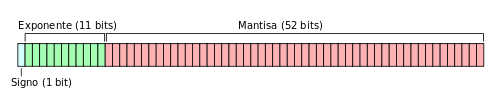
\includegraphics[scale = 0.68]{imagenes/ieee.png}~\\[0.25cm]
\end{center}

\begin{itemize}
	\item \textbf{Signo} ($s$) - 1 bit. El número representado es positivo si $s = 0$ y negativo si no.
	
	\item \textbf{Exponente} ($e$) - 11 bits. La base del exponente es 2. Para poder representar números con valor absoluto menor a 1 es necesario admitir exponentes negativos. Por esto, el exponente está representado en exceso a $2^{10} - 1$, es decir, el exponente del número representado será $(e)_{2} - (2^{10} - 1)$. Como $e$ tiene 11 bits entonces $0 \leq (e)_{2} \leq 2^{11} - 1 \Rightarrow -(2^{10} - 1) \leq (e)_{2} - (2^{10} - 1) \leq 2^{11} - 1 - (2^{10} - 1) \Rightarrow -2^{10} + 1 \leq (e)_{2} - (2^{10} - 1) \leq 2^{10}$.
	
	\item \textbf{Mantisa} ($m$) - 52 bits. Se considera una mantisa normalizada, i. e., el número representado tiene mantisa $(1, m)_{2}$.
\end{itemize}

En definitiva, el número representado es 

\[(-1)^s \cdot (1, m)_2 \cdot 2^{(e)_2 - (2^{10} - 1)}\]

%El mínimo número positivo está dado por $s = 0$, $e = \underbrace{0 \cdots 0}_{11\text{ bits}}$, $m = \underbrace{0 \cdots 0}_{52 \text{ bits}}$, que representa
%
%\[min^{+} = (-1)^0 \cdot 1 \cdot 2^{-1023} = 2^{-1023}\]
%
%El máximo positivo está dado por $s = 0$, $e = \underbrace{1 \cdots 1}_{11\text{ bits}}$, $m = \underbrace{1 \cdots 1}_{52 \text{ bits}}$, que representa
%
%\begin{align*}
%max^{+} &= (-1)^0 \cdot (1, 1 \cdots 1)_{2} \cdot 2^{(1 \cdots 1)_{2} - (2^{10} - 1)}\\
%&= \left(\sum_{i = 0}^{52} \left(\frac{1}{2}\right)^i\right) 2^{2^{11} - 1 - (2^{10} - 1)}\\
%&= \frac{1 - (1 / 2)^{53}}{1 - 1 / 2} 2^{1024}\\
%&= 2^{1024}\left(2 - (1 / 2)^{52}\right)\\
%&\approx 2^{1025}
%\end{align*}
%
%En el estándar IEEE, estos no son en realidad el mínimo y máximo valor positivo representable, debido a que los exponentes $e = 0$ y $e = \underbrace{1 \cdots 1}_{11 \text{ bits}}$ están reservados para valores especiales. De todos modos, $min^+$ y $max^+$ se aproximan bastante a los reales, y sirven para hacernos una idea de cuán chico o cuán grande puede ser un número representable en este sistema.
%
%Dado que el bit $s$ determina el signo del número, la representación es simétrica respecto del cero. Por lo tanto, los números negativos representables de menor y mayor absoluto son aproximadamente $- min^+$ y $- max^+$ respectivamente.

\begin{defi}
Decimos que un cómputo genera \emph{underflow} si su resultado es menor que el mínimo positivo representable, en módulo. Análogamente, decimos que genera \emph{overflow} si su resultado es mayor que el máximo positivo representable, en módulo.
\end{defi}

\subsection{Aproximación de los reales mediante números de máquina}

En esta sección estudiaremos cuán eficaz es la aproximación de un número real mediante un sistema con las características del presentado previamente. El tipo de sistemas a los que nos referimos son representaciones de punto flotante con una longitud de mantisa fija y exponente acotado.

Supongamos que nuestro conjunto de números de máquina es

\[\mathcal{M} = \{x \in \mathbb{R} : x = \pm (0, d_1 d_2 \cdots d_k) \cdot 10^e, 0 \leq d_i \leq 9, d_1 \neq 0, e_1 \leq e \leq e_2\}\]

dadas ciertas constantes $k$, $e_1$ y $e_2$. Esta es una representación normalizada con mantisa de $k$ dígitos y exponente entre $e_1$ y $e_2$. Es un sistema decimal y no binario como el de la IEEE, porque así será más fácil razonar sobre él. Todos los resultados que veremos en esta sección aplican, mutatis mutandi, a un sistema similar que utilice una base $b > 1$ cualquiera.

También por simplicidad, asumiremos que $e_1 = -\infty$ y $e_2 = +\infty$. Esto ahorra hablar del rango en el que corre el exponente, lo cual, como veremos, no hace a la esencia de los resultados.

\begin{defi}
Si $x \in \mathbb{R}$ es cualquiera, no necesariamente de máquina, llamamos $fl(x)$ a la aproximación de $x$ vía números de máquina. 
\end{defi}

Es definición depende del modo en que realicemos la aproximación. Consideremos la escritura

\[x = (0, d_1 \cdots d_kd_{k + 1} \cdots) \cdot 10^e\]
	
con $d_1 \neq 0$ (esta escritura es única dado que $d_1 \neq 0$). Entonces dos formas de aproximar $x$ son:

\begin{itemize}
	\item \textbf{Truncamiento.} Simplemente descartamos los dígitos $d_{k + 1}, d_{k + 2}, \cdots$, para obtener
	
	\[fl(x) = (0, d_1 \cdots d_k) \cdot 10^e\]

	\item \textbf{Redondeo.} Si $d_{k + 1} < 5$ entonces truncamos. Si no, sumamos $0,\underbrace{0 \cdots 05}_{k + 1 \text{ dígitos}} \cdot 10^e = 5 \cdot 10^{-(k + 1)} \cdot 10^e$ a $x$ y truncamos. En este último caso lo que queda es
	
	\[fl(x) = [(0, d_1 \cdots d_k) + 10^{-k}] \cdot 10^e\]

\end{itemize}

Una forma equivalente de enunciar estos criterios es la siguiente. Sea $x^{-}$ es el máximo número de máquina menor o igual que $x$. Análogamente, sea $x^{+}$ el mínimo número de máquina mayor o igual que $x$. Entonces, el truncamiento aproxima por $x^-$ mientras que el redondeo aproxima por aquel valor de $x^-$ o $x^+$ más cercano a $x$.

En general, las computadoras utilizan la aproximación por redondeo.

\subsection{Distribución de los números de máquina sobre la recta real}

\begin{obs}
Un número de máquina con exponente $e$ cae en el intervalo $[10^{e - 1}, 10^e)$.
\end{obs}

\begin{lema}
\label{lema:suc}
Dado $x \in \mathcal{M}$ con exponente $e$, el número de máquina que lo sucede es $x' = x + 10^{-k} \cdot 10^e$.

\begin{proof}
Por la observación anterior, $x$ cae en el intervalo $[10^{e - 1}, 10^e)$. Si $x$ es el máximo número de máquina en dicho intervalo, entonces $x'$ es el número de máquina más pequeño en $[10^e, 10^{e + 1})$, i. e., $x' = (0,1) \cdot 10^{e + 1}$. En caso contrario, el sucesor $x'$ también cae en $[10^{e - 1}, 10^e)$, con lo cual tiene exponente $e$. Lo mínimo que puede incrementarse la mantisa de $x$ es $0,\underbrace{0 \cdots 01}_{k \text{ dígitos}}$, con lo cual $x' = x + (0,\underbrace{0 \cdots 01}_{k \text{ dígitos}}) \cdot 10^e = x + 10^{-k} \cdot 10^e$.
\end{proof}
\end{lema}

La distribución de $\mathcal{M}$ no es uniforme sobre la recta real. Para ver por qué, contemos la cantidad de números de máquina que hay en el intervalo $[10^{i}, 10^{i + 1})$ con $i \in \mathbb{Z}$ una constante entera.

\begin{propo}
\label{propo:dist}
La cantidad de números de máquina $x \in \mathcal{M}$ tal que $x \in [10^i, 10^{i + 1})$ es $9 \cdot 10^{k - 1}$.

\begin{proof}
El menor número de máquina en $[10^{i}, 10^{i + 1})$ es $(0,1) \cdot 10^{i + 1} = 10^{i}$, y el mayor es $(0,99\cdots 99) \cdot 10^{i + 1}$. Entre estos dos están

\begin{center}
$(0,10\cdots 00) \cdot 10^{i + 1}$\\
$(0,10\cdots 01) \cdot 10^{i + 1}$\\
	$\vdots$\\
$(0,99\cdots 98) \cdot 10^{i + 1}$\\
$(0,99\cdots 99) \cdot 10^{i + 1}$\\
\end{center}

Observemos que estos son todos los números de máquina positivos con exponente $i + 1$. Afirmamos que no hay otros números de máquina en $[10^i, 10^{i + 1})$. Si un número en $\mathcal{M}$ positivo tiene exponente menor o igual que $i$, como la mantisa es estrictamente menor que 1, entonces el número será estrictamente menor que $10^i$. En caso contrario, si tiene exponente mayor o igual que $i + 2$, como el primer dígito decimal de la mantisa es no nulo, el número será al menos $10^{i + 1}$.

Para ver cuántos números hay en esta lista, notemos que hay tantos como números enteros entre $10^{k - 1}$ y $10^{k} - 1$, y estos son $9 \cdot 10^{k - 1}$.
\end{proof}
\end{propo}

\begin{coro}
Los números de máquina no están uniformemente distribuidos.

\begin{proof}
Como $\#(\mathcal{M} \cap [10^i, 10^{i + 1})) = 9 \cdot 10^{k - 1}$ no depende de $i$, resulta que en los intervalos $[1, 10)$, $[10, 100)$, $[100, 1000)$, $\cdots$, $[10^i, 10^{i + 1})$, $\cdots$, hay igual cantidad de números de máquina.
\end{proof}
\end{coro}

Intuitivamente, cuanto más nos alejemos de 0, más esparcidos estarán los números de máquina. Lo próximo que queremos es medir cuán esparcidos están, según el intervalo $[10^i, 10^{i + 1})$ en el que caigan.

\begin{lema}
Sea $x \in \mathcal{M} \cap [10^i, 10^{i + 1})$ y sea $x'$ su sucesor. Entonces $x' - x = 10^{i + 1 - k}$.

\begin{proof}
Como el exponente de $x$ es $i + 1$ entonces $x' = x + 10^{-k} \cdot 10^{i + 1}$, y concluimos $x' - x = 10^{i + 1 - k}$.
\end{proof}
\end{lema}

\begin{coro}
En cada intervalo $[10^i, 10^{i + 1})$ los números de máquina consecutivos estan equiespaciados.
\end{coro}

Más aún, a medida que $i$ crece, la brecha entre elementos consecutivos en $[10^i, 10^{i + 1})$ se hace mayor. De aquí se deduce que la distribución de los números de máquina tiene el siguiente aspecto
\\[0.5cm]
\begin{figure}[h]
\centering
\input{imagenes/distribucion.pdf_tex}
\end{figure}\\[0.5cm]

Esta distribución puede parecer extraña. Contrariamente a lo intuitivo, que haría pensar que una distribución uniforme sería más útil, esta distribución exponencial de los números de máquina resulta práctica pues se basa en la idea de que cuanto más chicos sean los números del rango en el que estamos trabajando, más pequeñas serán las variaciones que estaremos interesados en hacer. Contrariamente, cuanto más grandes sean los números con los que trabajemos, más grandes serán las variaciones con las que vayamos a trabajar. Esta noción se formaliza en la siguiente sección.

\subsection{Error absoluto y error relativo}

\begin{defi} Sea $x \in \mathbb{R}$. Sea $x^* \in \mathbb{R}$ un valor que pretende aproximar a $x$. 
\begin{itemize}
	\item El error absoluto de aproximar $x$ por $x^*$ es $|x - x^*|$.
	\item El error relativo de aproximar $x$ por $x^*$ es $\frac{|x - x^*|}{|x|}$.
\end{itemize}
\end{defi}

Notemos que la diferencia entre estas dos medidas de error, es que el absoluto no contempla el tamaño del valor que estamos aproximando mientras que el relativo sí lo hace. Esto determina que, en general, el error absoluto no sea una buena medida para el error, puesto que en ciertos contextos podemos tener un error absoluto aparentemente grande aunque la aproximación sea buena (por ejemplo, si aproximáramos la distancia entre la Tierra y la Luna con un error absoluto de 1000m) y en otros contextos podemos tener un error absoluto aparentemente chico aunque la aproximación sea mala (por ejemplo, si aproximáramos el perímetro de una célula vegetal con un error absoluto de 1mm).

Supongamos que queremos aproximar una magnitud que vale $x = 1000$, y nos piden que el error relativo sea a lo sumo $0,01$. Si nuestra medición es $x^* = 990$ entonces el error relativo será

\[\frac{|x - x^*|}{|x|} = \frac{10}{1000} = 0,01\]

con lo cual esta medición satisface lo pedido. Es fácil ver que cualquiera sea $x^* \in [990, 1010]$ cumple.

Supongamos que ahora estamos buscando medir una magnitud $x = 10$. La precisión buscada es la misma que antes, lo cual tiene sentido pues está expresada en términos relativos. Notemos que la medición $x^* = 9$ no será aceptada, porque el error relativo será de $0.1$. Refinando la medición a $x^* = 9.9$ conseguimos un error relativo de $0.01$ y es claro que cualquier valor $x^* \in [9.9; 10.1]$ no sobrepasa este error.

En ambas situaciones los errores relativos eran los mismos, sin embargo la diferencia en valor absoluto entre $x$ y los valores de $x^*$ aceptados era mucho mayor en el primer caso que en el segundo caso. La discusión del final de la sección anterior cobra ahora mucho más sentido.

A continuación estudiamos el error relativo al aproximar un número real por un número de máquina.

\begin{propo}
Si $fl(x)$ se obtiene truncando $x$ entonces

\[\frac{|x - fl(x)|}{|x|} \leq 10^{1 - k}\]

\begin{proof}
Supongamos sin pérdida de generalidad que $x > 0$. Sea $x = (0,d_1 \cdots d_k d_{k + 1} \cdots) \cdot 10^e$. Entonces

\begin{align*}
\frac{|x - fl(x)|}{|x|} &= \frac{|(0,d_1\cdots d_k d_{k + 1}\cdots) \cdot 10^e - (0,d_1 \cdots d_k) \cdot 10^e|}{|(0,d_1\cdots d_k d_{k + 1} \cdots) \cdot 10^e|}\\
&= \frac{(0,0\cdots 0 d_{k + 1} d_{k + 2} \cdots )}{(0,d_1 \cdots d_k d_{k + 1} \cdots)}
\end{align*}

Como $(0,d_1 \cdots d_k d_{k + 1} \cdots) \geq 0,1 = 10^{-1}$ y $(0,0\cdots 0 d_{k + 1}d_{k + 2}\cdots) \leq 0,\underbrace{0\cdots 01}_{k \text{ dígitos}} = 10^{-k}$, entonces

\[\frac{|x - fl(x)|}{|x|} \leq 10 \cdot 10^{-k} = 10^{1 - k}\]

\end{proof}
\end{propo}

\begin{propo}
\label{propo:er}
Si $fl(x)$ se obtiene redondeando $x$ entonces

\[\frac{|x - fl(x)|}{|x|} \leq \frac{1}{2} \cdot 10^{1 - k}\]

\begin{proof}
Separamos en casos, según el valor de $d_{k + 1}$.

Si $d_{k + 1} < 5$ entonces $fl(x) = (0,d_1 \cdots d_k) \cdot 10^e$. Entonces, haciendo la misma cuenta que antes,

\[\frac{|x - fl(x)|}{|x|} = \frac{(0,0\cdots 0 d_{k + 1} d_{k + 2} \cdots )}{(0,d_1 \cdots d_k d_{k + 1} \cdots)}\]

Como $d_{k + 1} < 5$ entonces $(0,0\cdots 0 d_{k + 1} d_{k + 2} \cdots) \leq 5 \cdot 10^{-(k + 1)}$. Luego

\[\frac{|x - fl(x)|}{|x|} \leq 5 \cdot 10^{-(k + 1)} \cdot 10 = \frac{10}{2} \cdot 10^{-k} = \frac{1}{2} \cdot 10^{1 - k}\]

Veamos el caso $d_{k + 1} \geq 5$. Ahora tenemos $fl(x) = [(0, d_1 \cdots d_k) + 10^{-k}] \cdot 10^e$. Entonces

\begin{align*}
\frac{|x - fl(x)|}{|x|} &= \frac{|(0,d_1\cdots d_k d_{k + 1}\cdots) - [(0,d_1\cdots d_k) + 10^{-k}]|}{(0,d_1\cdots d_k d_{k + 1} \cdots)}\\
&= \frac{|(0,0\cdots 0d_{k + 1}d_{k + 2}\cdots) - 10^{-k}|}{(0,d_1\cdots d_k d_{k + 1} \cdots)}\\
&= \frac{10^{-k} - (0,0\cdots 0d_{k + 1}d_{k + 2}\cdots)}{(0,d_1\cdots d_k d_{k + 1} \cdots)}\\
&= \frac{(0,0\cdots 0(9 - d_{k + 1})(9 - d_{k + 2}) \cdots)}{(0,d_1\cdots d_k d_{k + 1} \cdots)}
\end{align*}

Como $d_{k + 1} \geq 5$ entonces $(0,0\cdots 0(9 - d_{k + 1})(9 - d_{k + 2}) \cdots ) \leq (0,\underbrace{0\cdots 0}_{k \text{ dígitos}}499\cdots) = 5 \cdot 10^{-(k + 1)}$. Luego

\[\frac{|x - fl(x)|}{|x|} \leq 5 \cdot 10^{-(k + 1)} \cdot 10 = \frac{1}{2} \cdot 10^{1 - k}\]

\end{proof}
\end{propo}

\begin{coro}
En una máquina con representación de punto flotante decimal con mantisa de $k$ dígitos, el error de redondeo es $\mathcal{O}(10^{-k})$.
\end{coro}

El máximo error relativo que se puede cometer, según lo calculado en la Proposición \ref{propo:er}, tiene un nombre particular.

\subsection{Epsilon de máquina}

\begin{defi}
Llamamos epsilon de máquina al máximo error relativo que puede cometerse por redondeo. Lo notamos $\varepsilon$.
\end{defi}

En el caso de la máquina $\mathcal{M}$ con la que venimos trabajando, el epsilon de máquina es $\varepsilon = \frac{1}{2} \cdot 10^{1 - k}$.

\begin{propo}
$\varepsilon$ es el mínimo real positivo $x$ tal que $fl(1 + x) \neq 1$.

\begin{proof}
La observación clave es que el número representable que sigue al 1 es $1 + 10^{-k} \cdot 10 = 1 + 10^{1 - k}$ (Lema \ref{lema:suc}). Entonces, el punto medio entre 1 y su sucesor es $1 + \frac{1}{2} \cdot 10^{1 - k}$. De aquí se deduce que si $0 \leq x < \frac{1}{2} \cdot 10^{1 - k}$ entonces al redondear $1 + x$ obtenemos $fl(1 + x) = 1$, y si $x = \frac{1}{2} \cdot 10^{1 - k}$ y redondeamos $1 + x$ obtenemos el sucesor. Entonces $x = \frac{1}{2} \cdot 10^{1 - k} = \varepsilon$ es el mínimo que cumple lo buscado.
\end{proof}
\end{propo}

\begin{obs}
La validez de este resultado proviene de la fuerte relación que hay entre la cota superior para el error relativo y la distancia entre 1 y el número de máquina que lo sucede.
\end{obs}

\begin{obs}
El epsilon de máquina no tiene ninguna relación con el mínimo real positivo representable. De hecho, el mínimo representable depende del rango en el que se mueve el exponente, y no de la precisión de la mantisa.
\end{obs}

%\begin{propo}
%Sea $\alpha \in \mathcal{M}$ cualquiera, que tiene exponente $e$. El mínimo real positivo $x$ tal que $fl(\alpha + x) \neq \alpha$ es $x = \varepsilon \cdot 10^{e - 1} = \mathcal{O}(\varepsilon |\alpha|)$.

%\begin{proof}
%El sucesor de $\alpha$ es $\alpha + 10^{-k} \cdot 10^e$. El punto medio entre estos dos números de máquina será $\alpha + \frac{1}{2} \cdot 10^{-k} \cdot 10^e = \alpha + \varepsilon \cdot 10^{e - 1}$. Entonces el mínimo $x$ será dicho punto medio $x = \varepsilon \cdot 10^{e - 1}$. 
%\end{proof}
%\end{propo}

La noción de $\varepsilon$ permite dar cotas superiores sobre el error cometido al realizar distintas operaciones en una máquina, independientemente de las características del sistema de representación de números que utilice la misma. Las cuatro operaciones estándar que realiza una computadora son,

\[x \oplus y = fl(fl(x) + fl(y))\]
\[x \ominus y = fl(fl(x) - fl(y))\]
\[x \otimes y = fl(fl(x) \times fl(y))\]
\[x \oslash y = fl(fl(x) / fl(y))\]

que representan, respectivamente, la suma, la resta, el producto y el cociente de dos números reales $x$ e $y$.

\begin{propo}
Sean $x, y \in \mathbb{R}$ no nulos, con igual signo. En cualquier máquina con suma $\oplus$, que utilice redondeo, vale

\[\frac{|(x + y) - (x \oplus y)|}{|x + y|} \leq 2\varepsilon + \varepsilon^2\]

\begin{proof}
En efecto,

\begin{align*}
\frac{|(x + y) - (x \oplus y)|}{|x + y|} &= \frac{|(x + y) - (x \oplus y)|}{|x + y|}\\
&= \frac{|(x + y) - fl(fl(x) + fl(y))|}{|x + y|}\\
&= \frac{|x + y - (fl(x) + fl(y)) + (fl(x) + fl(y)) - fl(fl(x) + fl(y))|}{|x + y|}\\
&= \frac{\left|x\frac{x - fl(x)}{x} + y \frac{y - fl(y)}{y} + (fl(x) + fl(y)) \frac{fl(x) + fl(y) - fl(fl(x) + fl(y))}{fl(x) + fl(y)}\right|}{|x + y|}\\
&\leq \frac{1}{|x + y|} \left(|x| \frac{|x - fl(x)|}{|x|} + |y| \frac{|y - fl(y)|}{|y|} + |fl(x) + fl(y)| \frac{|fl(x) + fl(y) - fl(fl(x) + fl(y))|}{|fl(x) + fl(y)|}\right)\\
&\leq \frac{1}{|x + y|} \left(|x|\varepsilon + |y| \varepsilon + |fl(x) + fl(y)| \varepsilon \right)\\
&= \frac{1}{|x + y|}\left(|x| + |y| + |fl(x) + fl(y)| \right)\varepsilon\\
&= \frac{1}{|x + y|}\left(|x| + |y| + \left|x \frac{fl(x) - x}{x} + y \frac{fl(y) - y}{y} + x + y\right|\right)\varepsilon\\
&\leq \frac{1}{|x + y|}\left(|x| + |y| + |x|\frac{|x - fl(x)|}{|x|} + |y| \frac{|y - fl(y)|}{|y|} + |x| + |y|\right)\varepsilon\\
&\leq \frac{1}{|x + y|}\left(2|x| + 2|y| + |x|\varepsilon + |y|\varepsilon \right)\varepsilon\\
&=\frac{1}{|x + y|}(|x| + |y|)(2 + \varepsilon)\varepsilon\\
&=\frac{|x| + |y|}{|x + y|}(2\varepsilon + \varepsilon^2)
\end{align*}

Como $x$ e $y$ tienen igual signo, $\frac{|x| + |y|}{|x + y|} = 1$, lo cual termina la demostración.
\end{proof}
\end{propo}

%\begin{propo}
%Sean $x, y \in \mathbb{R}$ no nulos. En cualquier máquina con producto $\otimes$, que utilice redondeo, vale

%\[\frac{|xy - x \otimes y|}{|xy|} \leq 3\varepsilon + 3\varepsilon^2 + \varepsilon^3\]

%\begin{proof}
%En efecto,

%\begin{align*}
%\frac{|xy - x \otimes y|}{|xy|} &= \frac{|xy - fl(fl(x)fl(y))|}{|xy|}\\
%&=\frac{\left|y(x - fl(x)) + fl(x)(y -fl(y)) + (fl(x)fl(y))\frac{fl(x)fl(y) -fl(fl(x)fl(y))}{fl(x)fl(y)}\right|}{|xy|}\\
%&\leq \frac{|x - fl(x)|}{|x|} + \frac{|fl(x)|}{|x|}\frac{|y - fl(y)|}{|y|} + \frac{|fl(x)fl(y)|}{|xy|} \frac{|fl(x)fl(y) - fl(fl(x)fl(y))|}{|fl(x)fl(y)|}\\
%&\leq \varepsilon + \frac{|fl(x)|}{|x|}\varepsilon + \frac{|fl(x)fl(y)|}{|xy|}\varepsilon\\
%&= \left(1 + \frac{|fl(x)|}{|x|} + \frac{|fl(x)|}{|x|}\frac{|fl(y)|}{|y|}\right)\varepsilon
%\end{align*}

%Notemos que $\frac{|fl(x)|}{|x|} = \frac{|fl(x) - x + x|}{|x|} \leq \frac{|fl(x) - x|}{|x|} + 1 \leq \varepsilon + 1$, y análogamente con $y$. Entonces

%\begin{align*}
%\frac{|xy - x \otimes y|}{|xy|} &\leq (1 + (\varepsilon + 1) + (\varepsilon + 1)^2)\varepsilon\\
%&= 3\varepsilon + 3\varepsilon^2 + \varepsilon^3
%\end{align*}

%\end{proof}
%\end{propo}

%Comparemos las cotas obtenidas para las dos operaciones. Como $\varepsilon$ es muy chico, tiene sentido descartar todos los términos salvo los lineales. Concluimos que, a lo sumo, la suma (de números de igual signo) introduce un error aproximado $2\varepsilon$ y el producto un error aproximado $3\varepsilon$.

\subsection{Errores de redondeo clásicos}

\subsubsection{Suma de números de órdenes muy distintos}

Supongamos que tenemos un número real de valor absoluto pequeño, y otro de valor absoluto grande. Entonces la suma de máquina de los dos puede hacer que el más pequeño desaparezca.

Para ejemplificar, supongamos que nuestra aritmética tiene una precisión de $k = 5$ dígitos de mantisa. Sean $x = 0,88888888 \cdot 10^7$ e $y = 0,1 \cdot 10^2$. Entonces

\begin{align*}
x \oplus y &= fl(fl(x) + fl(y))\\
&= fl(0,88888 \cdot 10^7 + 0,1 \cdot 10^2)\\
&= fl(0,888881 \cdot 10^7)\\
&= 0,88888 \cdot 10^7
\end{align*}

El término $x$ ha absorbido a $y$. 

\subsubsection{Resta de números cercanos}

Al restar dos números cercanos, el resultado estará próximo a cero, lo que puede ocasionar que se pierdan dígitos significativos. Este fenómeno se conoce como \emph{cancelación catastrófica}, y tiene un gran impacto en el error relativo.

A modo de ejemplo, supongamos nuevamente que la precisión es de $k = 5$ dígitos, y sean que $x = 0,12346923$ e $y = 0,12345175$ entonces

\begin{align*}
x \ominus y &= fl(fl(x) - fl(y))\\
&= fl(0,12347 - 0,12345)\\
&= fl(0,00002)\\
&= 0,00002
\end{align*}

Sin embargo $x - y = 0,00001748$, lo que muestra que hemos perdido 3 dígitos significativos del resultado en la operación con redondeo.

\subsubsection{Multiplicación por números grandes o dividisión por números pequeños}

En este caso, se produce una amplificación del error absoluto acarreado. Supongamos que $x^*$ es una aproximación de máquina de $x$. Dividiendo a $x^*$ por un número muy pequeño, digamos $10^{-n}$ para cierto $n > 0$, obtenemos el número de máquina $x^* / 10^{-n}$ que aproxima a $x / 10^{-n}$ con un error absoluto de

\[|x^* / 10^{-n} - x / 10^{-n}| = |x^* - x| \cdot 10^{n}\]

El error absoluto $|x^* - x|$ del primer redondeo se ve amplificado en un factor de $10^n$.

\subsection{Generalización}

Como hemos dicho al principio de esta sección, hemos estudiado la representación de los números de máquina utilizando un sistema de base 10 exclusivamente por comodidad. Todos los resultados que vimos son fácilmente generalizables a una base arbitraria $b > 1$. A modo de ejemplo, en un conjunto análogo a $\mathcal{M}$ pero de base 2, el epsilon de máquina resulta ser $\varepsilon = \frac{1}{2} \cdot 2^{1 - k} = 2^{-k}$. 

Otro ejemplo interesante es la representación IEEE de precisión doble, cuyo conjunto de números de máquina es similar a $\mathcal{M}$ pero es de base 2 y tiene $k = 52 + 1$ dígitos de precisión (52 dígitos de mantisa más 1 dígito de precisión que agrega la normalización de la misma). Entonces, el epsilon de máquina en una computadora que use representación IEEE de precisión doble será $\varepsilon = 2^{-53}$. Éste es el máximo error relativo que una computadora típica cometerá por redondeo.
\newpage
\section{Ceros de función}

\subsection{Problema}

Dada $f : \mathbb{R} \to \mathbb{R}$, buscamos un $x^* \in \mathbb{R}$ tal que $f(x^*) = 0$. El número $x^*$ se llama cero o raíz de $f$.

En ciertos casos, como por ejemplo para $f(x)$ un polinomio de grado menor o igual que 2, el problema tiene una solución que sabemos calcular en forma exacta. En otros casos, por ejemplo para $f(x) = e^x - \ln(x^2)$, no parece tan claro cómo calcular una raíz, si es que existe una.

\subsection{Propuesta}

Para calcular una raíz, construiremos una sucesión $\{x_n\}_{n \in \mathbb{N}_0}$ de modo tal que $x_n \xrightarrow[n \to \infty]{} x^*$. Más aún, definiremos dicha sucesión en forma recurrente, de modo tal que a partir de $x_0$ podamos computar $x_1$, luego $x_2$ y así sucesivamente. Esto nos da un método iterativo, en el cual a medida que el número de iteraciones $n$ crece, la aproximación $x_n$ de $x^*$ es cada vez mejor, en el sentido de que el valor absoluto $|x_n - x^*|$ es cada vez más pequeño.

Sin saber aún cómo construir $\{x_n\}_n$, surgen algunas preguntas:

\begin{enumerate}
	\item ¿Cuán rápido convergerá $x_n$ a $x^*$? En otras palabras, ¿con qué velocidad la diferencia $|x_n - x^*|$ converge a 0?

	\item ¿Cuánto es necesario iterar para obtener una buena aproximación? Recordemos que la raíz $x^*$, a la que queremos converger, no es conocida de antemano, con lo cual, en general, no sabemos cuán cerca está $x_n$ de $x^*$ en un instante dado de la iteración.
	
	\item Dado que no podemos iterar infinitamente, necesitamos establecer criterios para decidir cuándo finalizar la iteración, que no dependan de la distancia entre $x_n$ y $x^*$.
\end{enumerate}

\subsection{Velocidad u orden de convergencia}

Como hemos planteado, nos interesa medir la velocidad con la que $\{x_n\}_n$ se aproxima a $x^*$.

\begin{defi}
Sea $\{x_n\}_n$ una sucesión que converge a $x^*$, pero $x_n \neq x^*$ para todo $n$. Decimos que $\{x_n\}_n$ tiene orden de convergencia $p > 0$ si

\[\lim\limits_{n \to \infty} \frac{|x_{n + 1} - x^*|}{|x_n - x^*|^p} = c \neq 0\]

para cierta constante $c \in \mathbb{R}$. Si $p = 1$ decimos que la convergencia es lineal.
Si $1 < p < 2$ decimos que la convergencia es supralineal.
Si $p = 2$ decimos que la convergencia es cuadrática.
\end{defi}

Observemos que si el orden de convergencia es $p$ entonces $|x_{n + 1} - x^*|$ es asintóticamente equivalente a $|x_n - x^*|^p$. Esto implica que, asintóticamente, el error absoluto se reduce polinomialmente, con exponente $p$.

Dado que algunas sucesiones convergen con velocidad variable, no siempre es posible aplicar la anterior definición. Hay una medida más general de la velocidad de convergencia, dada por la siguiente

\begin{defi}
Sea $\{\alpha_n\}_n$ convergente a $\alpha$. Sea $\{\beta_n\}_n$ convergente a 0. Decimos que $\{\alpha_n\}_n$ tiene orden de convergencia $\mathcal{O}(\beta_n)$ (o que $\alpha_n$ converge tan rápido como $\beta_n$) si existe una constante $c > 0$ tal que $\left|\alpha_n - \alpha \right| \leq c \beta_n$ para todo $n$ suficientemente grande. 

En este caso, si $\{\beta_n\}_n$ tiene orden de convergencia $p$, decimos que $\{\alpha_n\}_n$ tiene orden de convergencia al menos $p$. 
\end{defi}

\subsubsection{Interpretación}

¿Qué significa que $\{x_n\}_n$ converja a $x^*$ con orden $p$? Llamemos $e_n = x_n - x^*$. Según la definición de antes, esto significa que $\lim\limits_{n \to \infty}{\frac{|e_{n + 1}|}{|e_n|^p}} = c$ para cierta constante $c \neq 0$. Que $c$ no sea infinito, significa que $|e_{n}|^p$ no tiende a 0 más rápido de lo que lo hace $|e_{n + 1}|$. Que $c$ sea no nulo, significa que $|e_{n + 1}|$ tampoco lo hace más rápido que $|e_{n}|^p$. Por lo tanto, $|e_{n + 1}|$ y $|e_{n}|^p$ convergen a 0 con la misma velocidad o, dicho de otro modo, son asintóticamente equivalentes.

A su vez, es posible interpretar el significado de esta velocidad, en términos prácticos. Dada la equivalencia asintótica de $|e_{n + 1}|$ y $|e_n|^p$, vamos a suponer que para $n$ suficientemente grande $|e_{n + 1}| \approx |e_n|^p$. Supongamos que hasta el término $n$-ésimo llevamos calculados $k$ dígitos decimales del valor $x^*$, es decir que $|e_n| \approx 10^{-k}$. Entonces, $|e_{n + 1}| \approx (10^{-k})^p = 10^{-kp}$, es decir que en el $(n + 1)$-ésimo término, la cantidad de decimales calculados se multiplica por $p$.

Entonces, por ejemplo, que una sucesión converja cuadráticamente significa, a nivel práctico, que la cantidad de dígitos decimales calculados se duplica a cada paso.

\subsection{Criterios de parada}
Respondemos a la tercera pregunta que nos hicimos previamente.

\begin{itemize}
	\item Fijar un número máximo $N$ de iteraciones.
	
	\item Fijar $\varepsilon > 0$ y terminar cuando $|x_n - x_{n - 1}| < \varepsilon$. 
	
	Esto es, terminar cuando los saltos de la sucesión sean chicos.
	
	Este criterio puede fallar. Por ejemplo, tomemos $x_n = \sum_{k = 1}^n \frac{1}{k}$ la sucesión de números armónicos. Como $x_n - x_{n - 1} = \frac{1}{n} \xrightarrow[n \to \infty]{} 0$ entonces para cualquier $\varepsilon > 0$ existirá un valor de $n$ suficientemente grande para el cual dos términos sucesivos disten menos de $\varepsilon$. Sin embargo, es bien sabido que los números armónicos divergen.
	
	\item Fijar $\varepsilon > 0 $ y terminar cuando $\frac{|x_n - x_{n - 1}|}{|x_{n - 1}|} < \varepsilon$. 
	
	Esto es, terminar cuando la sucesión no de saltos demasiado grandes en términos relativos.
	
	\item Fijar $\varepsilon > 0$ y terminar cuando $|f(x_n)| < \varepsilon$. 
	
	Este criterio se basa en que si $x_n$ converge a una raíz, entonces cuando la sucesión converja, $f(x_n)$ será pequeño.
	
	También puede fallar. Por ejemplo, en el caso en que $f(x)$ está muy cerca de cero en un punto pero no tiene una raíz en el entorno (e. g. $f(x) = \frac{1}{x}$).
	
	\item Fijar $\varepsilon > 0$ y terminar cuando $|f(x_n) - f(x_{n - 1})| < \varepsilon$.
	
	\item Fijar $\varepsilon > 0$ y terminar cuando $\frac{|f(x_n) - f(x_{n - 1})|}{|f(x_{n - 1})|} < \varepsilon$.
\end{itemize}

Dado que todos estos criterios son heurísticos, pueden fallar. La elección del criterio adecuado dependerá del contexto.

A continuación exploraremos algunas formas de encontrar una tal sucesión $\{x_n\}_n$ que converja a una raíz.

\subsection{Método de Bisección}

Supongamos que tenemos una función $f:[a, b] \to \mathbb{R}$ contínua, a la que le queremos calcular una raíz. Supongamos, además, que $f(a)f(b) < 0$, es decir, $f(a)$ y $f(b)$ tienen signos opuestos. Consideremos el Algoritmo \ref{algo:bisec}, que asume que estamos en estas condiciones.

\begin{algorithm}
\label{algo:bisec}
\dontprintsemicolon

%\SetKwInOut{Input}{input}
%\SetKwInOut{Output}{output}

%\Input{}
%\Output{}

Sean $a_0 = a$, $b_0 = b$\;
\For{$k = 1$ \KwTo $N$}{
	$c_{k - 1} = \frac{a_{k - 1} + b_{k - 1}}{2}$\;
	Si $f(c_{k - 1})$ cumple con el criterio de parada, terminar\;
	Si $f(c_{k - 1})f(a_{k - 1}) < 0$, entonces $a_k = a_{k - 1}$, $b_k = c_{k - 1}$\;
	Si $f(c_{k - 1})f(b_{k - 1}) < 0$, entonces $a_k = c_{k - 1}$, $b_k = b_{k - 1}$\;
}

\caption[]{Método de Bisección}
\end{algorithm}

El algoritmo determina tres sucesiones $\{a_n\}_n$, $\{b_n\}_n$ y $\{c_n\}_n$. En cada paso elige a $c_n$ como el punto medio entre $a_n$ y $b_n$. 

\begin{obs}
Las lineas 5 y 6 garantizan que

\begin{itemize}
\item $a_n \leq c_n \leq b_n$ para todo $n$.

\item $f(a_n)f(b_n) < 0$ para todo $n$.

\item La sucesión $\{a_n\}_n$ es creciente, mientras que $\{b_n\}_n$ es decreciente.
\end{itemize}
\end{obs}

Veamos que la sucesión $\{c_n\}_n$ converge a una raíz de $f$.

\begin{lema}
\label{lema:sucs}
\[b_n - a_n \leq \frac{b_0 - a_0}{2^n}\]

\begin{proof}
Por inducción en $n \in \mathbb{N}_0$.

Si $n = 0$, no hay nada que ver.

Sea $n > 0$. Es fácil ver que las lineas 5 y 6 del algoritmo eligen $a_n$ y $b_n$ de modo tal que $b_n - a_n \leq \frac{b_{n - 1} - a_{n - 1}}{2}$. Por hipótesis inductiva, $b_{n - 1} - a_{n - 1} \leq \frac{b_0 - a_0}{2^{n - 1}}$ y usando la desigualdad anterior llegamos al resultado buscado.
\end{proof}
\end{lema}

En particular, esto muestra que $\lim\limits_{n \to \infty}(b_n - a_n) = 0$.

\begin{propo}
La sucesion $\{c_n\}_n$ es convergente. Más aún $\lim\limits_{n \to \infty} c_n$ es una raíz de $f$.

\begin{proof}
Como $a_n \leq b_n$ para todo $n$, y $\{b_n\}_n$ es decreciente, entonces $\{a_n\}_n$ está acotada superiormente, por ejemplo por $b_0$. Además $\{a_n\}_n$ es creciente. Luego, es una sucesión convergente. Sea $\ell = \lim\limits_{n \to \infty} a_n$.

Análogamente, $\{b_n\}_n$ es una sucesión decreciente acotada inferiormente, por ejemplo por $a_0$, con lo cual es convergente. Luego $0 = \lim\limits_{n \to \infty} (b_n - a_n) = \lim\limits_{n \to \infty} b_n - \ell$, con lo cual $\lim\limits_{n \to \infty} b_n = \ell$.

Como $a_n \leq c_n \leq b_n$, entonces $\{c_n\}_n$ está acotada entre dos sucesiones que convergen al mismo límite. Por Sandwich, debe ser $\lim\limits_{n \to \infty} c_n = \ell$. En definitiva, $\{a_n\}_n$, $\{b_n\}_n$ y $\{c_n\}_n$ convergen las tres y tienen el mismo límite.

Falta ver que $f(\ell) = 0$. Si fuera $f(\ell) > 0$ entonces, como $f$ es contínua y $a_n$ tiende a $\ell$, tendríamos $f(a_n) > 0$ para todo $n$ suficientemente grande. Análogamente, $f(b_n) > 0$ para todo $n$ suficientemente grande. Pero esto contradice el hecho de que $f(a_n)f(b_n) < 0$ para todo $n$. Análogamente, no puede ser $f(\ell) < 0$. Entonces no queda otra que $f(\ell) = 0$.

\end{proof}
\end{propo}

Esto demuestra que el método siempre converge a una raíz de la función. En lo que sigue llamaremos $x^* = \lim\limits_{n \to \infty} c_n$.

\begin{obs}
De la monotonía de las sucesiones se deduce que $a_n \leq x^* \leq b_n$ para todo $n$.
\end{obs}

\begin{propo}
\[|c_n - x^*| \leq \frac{b_0 - a_0}{2^{n + 1}}\]

\begin{proof}
Como $a_n \leq x^* \leq b_n$ y $c_n$ es el punto medio, entonces $|c_n - x^*| \leq \frac{b_n - a_n}{2}$. Por el Lema \ref{lema:sucs}, se deduce $|c_n - x^*| \leq \frac{b_0 - a_0}{2^{n + 1}}$.
\end{proof}
\end{propo}

\begin{coro}
El orden de convergencia de $\{c_n\}_n$ es al menos lineal.

\begin{proof}
Se desprende de que $\frac{b_0 - a_0}{2^{n + 1}}$ converge linealmente.
\end{proof}
\end{coro}

\subsubsection{Ventajas y desventajas}

\paragraph{Ventajas}

\begin{itemize}
	\item Para cada $a_n$ y $b_n$, nos alcanza con conocer el signo de $f(a_n)$ y el de $f(b_n)$ con lo cual podría no ser necesario evaluar la función $f$ en esos puntos. Esto es conveniente en contextos en los cuales la evaluación es una operación costosa y es posible conocer el signo por alguna vía sencilla.
	\item Tenemos una cota para el error absoluto.
	\item Es fácil encontrar puntos iniciales $a_0$ y $b_0$ factibles.
\end{itemize}

\paragraph{Desventajas}

\begin{itemize}
	\item Asegura una convergencia de orden al menos lineal, aunque puede resultar lenta.
\end{itemize}

\subsection{Problemas de punto fijo}

\begin{defi}
Sea $g: [a, b] \to \mathbb{R}$. Un punto $p \in [a, b]$ se llama punto fijo de $g$ si $g(p) = p$.
\end{defi}

Un problema de cálculo de raíces de una función $f(x)$ puede ser transformado en un problema de punto fijo. Por ejemplo si $g(x) = x + f(x)$ entonces $p$ es raíz de $f$ si y solo si $p$ es punto fijo de $g$.

La conveniencia de transformar el problema de cálculo de una raíz en un problema de punto fijo, se debe a que se conocen varios métodos para resolver esto último, como veremos a continuación.

\begin{propo}
Sea $g:[a, b] \to [a, b]$ contínua. Entonces $g$ tiene punto fijo en $[a, b]$. Si además es derivable y $|g'(x)| < 1$ para todo $x \in (a, b)$, entonces el punto fijo es único.

\begin{proof}
Primero veamos que $g$ tiene un punto fijo en $[a, b]$. Notemos que como $a \leq g(x) \leq b$, entonces $g(a) \geq a$ y $g(b) \leq b$. Si $g(a) = a$, listo. Si no, $g(a) > a$. Análogamente, si $g(b) = b$, terminamos. Si no, $g(b) < b$. Tenemos, entonces, $g(a) - a > 0$ y $g(b) - b < 0$.

Consideremos $f(x) = g(x) - x$. Por lo anterior, $f(a) > 0$ y $f(b) < 0$. Además $f$ es contínua en $[a, b]$ pues $g$ lo es. Luego, por Teorema de Bolzano, existe $p \in (a, b)$ tal que $f(p) = 0$, es decir que $g(p) - p = 0$ o bien $g(p) = p$, con lo cual $p$ es un punto fijo de $g$.

Veamos la unicidad. Sean $p_1, p_2 \in [a, b]$ puntos fijos de $g$, entonces $g(p_1) = p_1$ y $g(p_2) = p_2$. Como $g$ es derivable, por el Teorema del Valor Medio tenemos que

\[|g(p_1) - g(p_2)| = \left|p_1 - p_2\right| \left|g'(\xi)\right|\]

para cierto $\xi$ entre $p_1$ y $p_2$. Pero $|g(p_1) - g(p_2)| = |p_1 - p_2|$, entonces

\[|p_1 - p_2| = \left|p_1 - p_2\right| \left|g'(\xi)\right|\]

Por hipótesis, $\left|g'(\xi)\right| < 1$, con lo cual no queda otra que $|p_1 - p_2| = 0$, i. e., $p_1 = p_2$.

\end{proof}
\end{propo}

Dadas estas condiciones de existencia y unicidad de punto fijo, construimos una sucesión convergente a un punto fijo.

\begin{propo}
\label{propo:ptofijo}
Sea $g:[a, b] \to [a, b]$ contínua y derivable, tal que existe una constante no negativa $k$ tal que $|g'(x)| \leq k < 1$ para todo $x \in (a, b)$. Sea $\{x_n\}_n$ una sucesión tal que 

%\[x_0 \in [a, b] \text{ y } x_{n + 1} = g(x_n) \text{ si }n \geq 0\] 
\[x_0 \in [a, b]\]
\[x_{n + 1} = g(x_n) \text{ si }n \geq 0\] 

Entonces $\{x_n\}_n$ converge al único punto fijo de $g$.

\begin{proof}
Por la Proposición anterior, $g$ posee un único punto fijo en $[a, b]$, que llamamos $p$. Observemos que como $g(x) \in [a, b]$ y $x_0 \in [a, b]$, entonces todo término de la sucesión cae en $[a, b]$.

Queremos ver que $\lim \limits_{n \to \infty} x_n = p$. Notemos que si $n > 0$,

\[|x_n - p| = |g(x_{n - 1}) - g(p)|\]

Como $g$ es derivable, por el Teorema del Valor Medio existe $\xi_{n - 1}$ entre $x_{n - 1}$ y $p$, tal que

\[|g(x_{n - 1}) - g(p)| = \left|x_{n - 1} - p\right| \left|g'(\xi_{n - 1})\right|\]

Como $\left|g'(\xi_{n - 1})\right| \leq k$ entonces

\[|g(x_{n - 1}) - g(p)| \leq \left|x_{n - 1} - p\right| k\]

Por la primera de las igualdades, concluimos que

\[|x_n - p| \leq \left|x_{n - 1} - p\right| k\]

Inductivamente, es fácil ver que

\[|x_n - p| \leq \left|x_0 - p\right| k^n\]

Como $0 \leq k < 1$, $\left|x_0 - p\right| k^n$ tiende a 0 a medida que $n \to \infty$. Por el Teorema del Sandwich, $\lim \limits_{n \to \infty} |x_n - p| = 0$, con lo cual $\lim \limits_{n \to \infty} x_n = p$.

\end{proof}
\end{propo}

Esta técnica para encontrar el punto fijo se llama \textit{iteración de punto fijo}. Bajo ciertas condiciones podemos asegurar el orden de convergencia de la sucesión.

\begin{propo}
\label{propo:conv}
Sea $g \in C^{r}([a, b])$ tal que $p \in (a, b)$ es punto fijo y

\[g'(p) = g''(p) = \cdots = g^{(r - 1)}(p) = 0\text{, } g^{(r)}(p) \neq 0\]

Entonces, si $x_{n + 1} = g(x_n)$ converge a $p$, su orden de convergencia es $r$.

\begin{proof}
Como $g \in C^r([a, b])$, consideramos el desarrollo de Taylor de $g$ de orden $r - 1$, centrado en $p$,

\[g(x) = g(p) + g'(p) (x - p) + \cdots + \frac{g^{(r - 1)}(p)}{(r - 1)!} (x - p)^{r - 1} + \frac{g^{(r)}(\xi_x)}{r!} (x - p)^r = g(p) + \frac{g^{(r)}(\xi_x)}{r!} (x - p)^r\]

con $\xi_x$ entre $x$ y $p$. Evaluando en $x_n$ obtenemos

\[g(x_n) = g(p) + \frac{g^{(r)}(\xi_n)}{r!} (x_n - p)^r\]

con $\xi_n$ entre $x_n$ y $p$. Como $g(x_n) = x_{n + 1}$ y $g(p) = p$,

\[x_{n + 1} - p = \frac{g^{(r)}(p)}{r!} (x_n - p)^r\]

o sea que

\[\frac{x_{n + 1} - p}{(x_n - p)^r} = \frac{g^{(r)}(p)}{r!}\]

Tomando límite en ambos miembros,

\[\lim\limits_{n \to \infty} \frac{x_{n + 1} - p}{(x_n - p)^r} = \frac{g^{(r)}(p)}{r!}\]

Como esta expresión converge, su módulo también lo hace, y

\[\lim\limits_{n \to \infty} \frac{|x_{n + 1} - p|}{|x_n - p|^r} = \frac{|g^{(r)}(p)|}{r!}\]

Como $g^{(r)}(p) \neq 0$ entonces el límite $\frac{|g^{(r)}(p)|}{r!}$ es no nulo. Luego, el orden de convergencia de $\{x_n\}_n$ es $r$.

\end{proof}
\end{propo}

%\subsection{Interpretación de la velocidad de convergencia}

\subsection{Método de Newton}

Supongamos que dada una $f: \mathbb{R} \to \mathbb{R}$, queremos hallar una raíz. Para esto queremos encontrar una función $g: \mathbb{R} \to \mathbb{R}$, cuya expresión involucre a $f$, de modo tal que los puntos fijos de $g$ sean raíces de $f$. Más aún, vamos a pedir que la iteración de punto fijo asociada a $g$ converja cuadráticamente.

Proponemos $g(x) = x - h(x)f(x)$ siendo $h$ una función que todavía no conocemos. Notemos que si $p$ es punto fijo de $g$ entonces $p = g(p) = p - h(p)f(p)$, con lo cual si $h(p) \neq 0$ resulta que $f(p) = 0$. Por lo tanto, todo punto fijo de $g$ es una raíz de $f$, sea cual sea la función $h$ tal que $h(p) \neq 0$.

Como queremos un orden de convergencia cuadrático, pedimos que $g'(p) = 0$. Como $g'(x) = 1 - h'(x)f(x) - h(x) f'(x)$, entonces

\begin{align*}
g'(p) = 0 &\Leftrightarrow 1 - h'(p)f(p) - h(p)f'(p) = 0\\
&\Leftrightarrow 1 - h(p)f'(p) = 0\\
&\Leftrightarrow h(p) = \frac{1}{f'(p)}
\end{align*}

suponiendo que $f'(p) \neq 0$. Entonces podemos tomar $h(x) = \frac{1}{f'(x)}$, que cumple $h(p) \neq 0$. Así, queda

\[g(x) = x - \frac{f(x)}{f'(x)}\]

con lo cual la iteración de punto fijo asociada es

\[x_{n + 1} = g(x_n) = x_n - \frac{f(x_n)}{f'(x_n)}\]

En lo que sigue vamos a ver que esta sucesión efectivamente converge a un punto fijo de $g$ (bajo ciertas condiciones), y lo hace cuadráticamente.

\begin{propo}
Sea $f \in C^2([a, b])$. Sea $p \in (a, b)$ tal que $f(p) = 0$, $f'(p) \neq 0$. Entonces existe $\delta > 0$ tal que toda sucesión $\{x_n\}_n$ con

%\[x_0 \in [p - \delta, p + \delta] \text{ y } x_{n + 1} = x_n - \frac{f(x_n)}{f'(x_n)} \text{ si } n \geq 0\]
\[x_0 \in [p - \delta, p + \delta]\]
\[x_{n + 1} = x_n - \frac{f(x_n)}{f'(x_n)} \text{ si } n \geq 0\]

está bien definida y converge.

\begin{proof}
Sea $g(x) = x - \frac{f(x)}{f'(x)}$.

\begin{itemize}
\item \textbf{$g$ está bien definida en un entorno de $p$.} Como $f'$ es contínua en $[a, b]$ y $p \in (a, b)$ entonces $f'$ es contínua en $p$. En particular, existe $\delta_1 > 0$ tal que $f'(x) \neq 0$ para todo $x \in [p - \delta_1, p + \delta_1]$.

\item \textbf{$g$ es estable en un entorno de $p$.} Notemos que $g'(x) = \frac{f(x)f''(x)}{f'(x)^2}$, que está bien definida en $[p - \delta_1, p + \delta_1]$.

Como $g'(p) = 0$ y $g'$ es contínua en $p$, entonces existe $\delta_2 > 0$, $\delta_2 \leq \delta_1$ tal que, para alguna constante $k$, $|g'(x)| \leq k < 1$ para todo $x \in (p - \delta_2, p + \delta_2)$.
 
Luego, si $x \in [p - \delta_2, p + \delta_2]$, utilizando el Teorema del Valor Medio, deducimos que

\[|g(x) - g(p)| = \left|g'(\xi_x)\right| \left| x - p \right|\]

para $\xi_x$ entre $x$ y $p$. Entonces $|g'(\xi_x)| < 1$. Como además $g(p) = p$ resulta que

\[|g(x) - p| < |x - p| \leq \delta_2\]

Luego $|g(x) - p| \leq \delta_2$, es decir que $g(x) \in [p - \delta_2, p + \delta_2]$.

\end{itemize}

Por lo tanto, $g: [p - \delta_2, p + \delta_2] \to [p - \delta_2, p + \delta_2]$ está bien definida y además $|g'(x)| \leq k < 1$ para todo $x \in (p - \delta_2, p + \delta_2)$. Poniendo $\delta = \delta_2$, una sucesión $\{x_n\}_n$ tal que $x_0 \in [p - \delta, p + \delta]$ y $x_{n + 1} = g(x_n) = x_n - \frac{f(x_n)}{f'(x_n)}$ está en las condiciones de la Proposición \ref{propo:ptofijo}, con lo cual converge a un punto fijo de $g$.

\end{proof}
\end{propo}

Observemos que este resultado sólo asegura la convergencia cuando comenzamos la iteración dentro de un entorno suficientemente chico del punto fijo. En general, no conocemos la localización del punto fijo así como tampoco cuán chico debe ser el entorno. Por esta razón, se suele partir desde un punto arbitrario, e iterar, revisando si se logra converger. En caso negativo, se elige otro punto de partida y se repite la iteración.

Otra forma de sortear el problema es aplicar, inicialmente, algunas iteraciones del método de Bisección y cuando el entorno que contiene a la raíz es suficientemente chico, proceder con Newton.

\begin{propo}
Sea $f \in C^2$ y $p \in \mathbb{R}$ una raíz de $f$. Sea $\{x_n\}_n$ la iteración de punto fijo dada por $x_{n + 1} = x_n - \frac{f(x_n)}{f'(x_n)}$. Supongamos que está bien definida y que nunca vale $p$. Si $e_n = x_n - p$, entonces

\[\frac{e_{n + 1}}{e_n^2} = \frac{1}{2} \frac{f''(\xi_n)}{f'(x_n)}\]

con $\xi_n$ un valor entre $x_n$ y $p$. Más aún, si $f'(p), f''(p) \neq 0$ y la iteración converge a $p$, entonces lo hace con orden cuadrático.

\begin{proof}

Para cada $n \in \mathbb{N}_0$, consideremos el desarrollo de Taylor de $f$ de orden 1 centrado en $x_n$,

\[f(x) = f(x_n) + f'(x_n) (x - x_n) + \frac{f''(\xi_n)}{2} (x - x_n)^2\]

con $\xi_n$ entre $x_n$ y $x$. Evaluando en $p$ obtenemos

\[f(p) = f(x_n) + f'(x_n) (p - x_n) + \frac{f''(\xi_n)}{2} (p - x_n)^2\]

con $\xi_n$ entre $x_n$ y $p$. Luego,

\[0 = f(x_n) - f'(x_n) e_n + \frac{f''(\xi_n)}{2} e_n^2\]

Con un poco de aritmética llegamos a la ecuación buscada,

\[\frac{e_{n + 1}}{e_n^2} = \frac{1}{2} \frac{f''(\xi_n)}{f'(x_n)}\]

Resta ver que si $f'(p) \neq 0$ y $\{x_n\}_n$ converge a $p$, entonces lo hace cuadráticamente. Para esto, debemos ver que $\frac{|e_{n + 1}|}{|e_n|^2}$ converge a una constante no nula. Tomando módulo en la ecuación anterior,

\[\frac{|e_{n + 1}|}{|e_n|^2} = \frac{1}{2} \frac{|f''(\xi_n)|}{|f'(x_n)|}\]

Como $f'$ es contínua, y $\lim\limits_{n \to \infty} x_n = p$, entonces

\[\lim\limits_{n \to \infty} f'(x_n) = f'(p) \neq 0\]

Por otro lado, como $\xi_n$ siempre cae entre $x_n$ y $p$, y $f''$ es contínua, resulta que

\[\lim\limits_{n \to \infty} f''(\xi_n) = f''(p)\]

Por lo tanto, estas dos últimas expresiones convergen en módulo y, más aún,

\[\lim\limits_{n \to \infty} \frac{|e_{n + 1}|}{|e_n|^2} = \lim\limits_{n \to \infty} \frac{1}{2}\frac{|f''(\xi_n)|}{|f'(x_n)|} = \frac{1}{2}\frac{|f''(p)|}{|f'(p)|} \neq 0\]

que es lo que queríamos probar.

\end{proof}
\end{propo}

\subsubsection{Interpretación geométrica}

Este método tiene una muy linda interpretación geométrica. Dada una función $f$, tomamos un punto $p_0$ y consideramos la recta tangente que pasa por el punto $(p_0, f(p_0))$. Definimos $p_1$ como la intersección entre dicha recta y el eje $x$. Ahora tomamos la recta tangente que pasa por el punto $(p_1, f(p_1))$ y definimos $p_2$ como la intersección entre esta recta y el eje $x$. Continuando de esta forma nos iremos aproximando cada vez más a una raíz $p$ de $f$. La siguiente imágen ilustra este proceso.

\begin{center}
	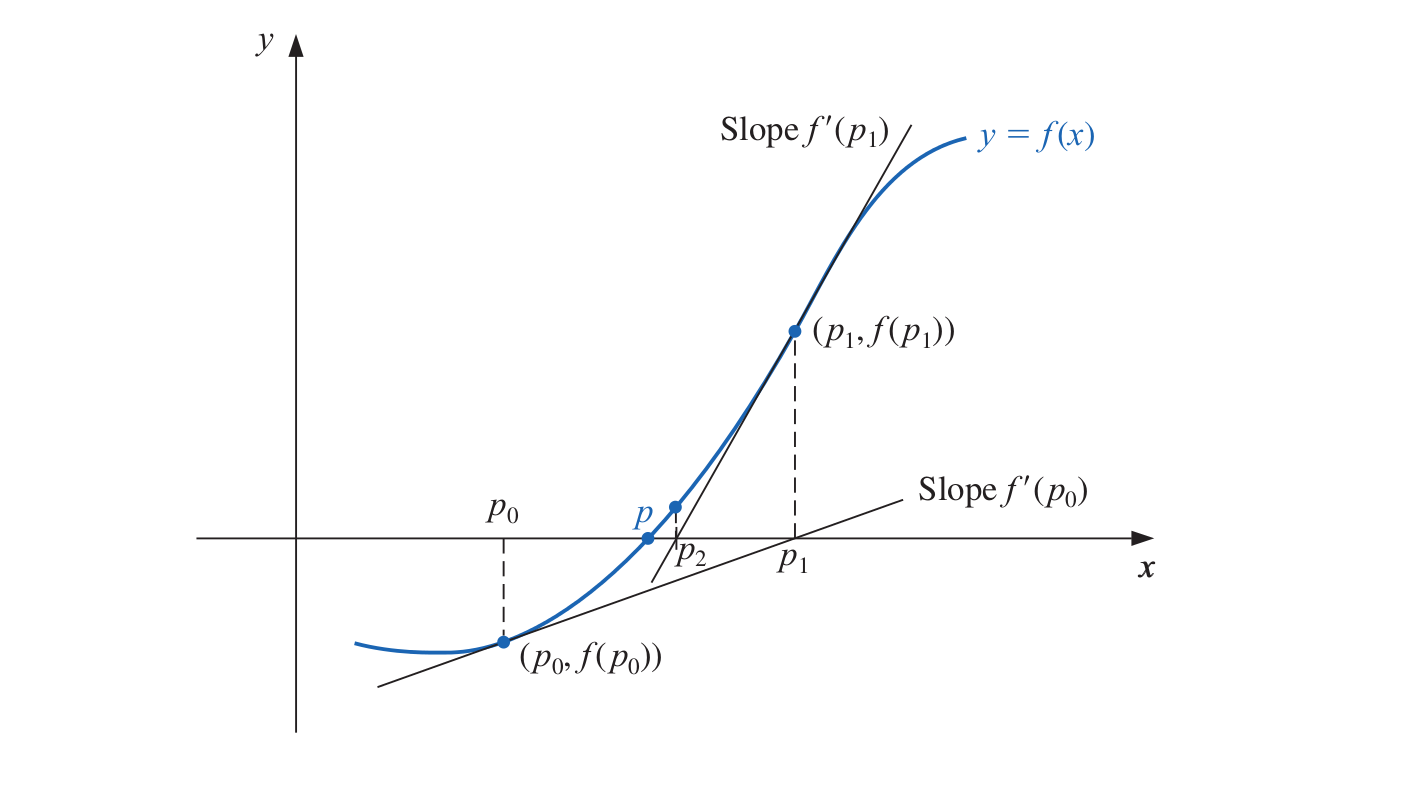
\includegraphics[scale = 0.27]{imagenes/newton.png}~\\[0.25cm]
\end{center}

Sea $\{x_n\}_n$ una iteración de Newton. Dado $x_n$, definimos $x_{n + 1}$ como la abscisa de la intersección entre la recta tangente a $f$ en $x_n$ y el eje $x$. La recta tangente a $f$ en $x_n$ es $y = f'(x_n)x + b$ siendo $b$ la ordenada al origen. Para $x = x_n$, esta recta toma el valor $y = f(x_n)$, con lo cual $f(x_n) = f'(x_n) x_n + b$, i. e., $b = f(x_n) - x_n f'(x_n)$. Luego, la recta tangente a $f$ en $x_n$ es

\[y = f'(x_n)x + f(x_n) - x_n f'(x_n)\]

La intersección entre esta recta y el eje $x$ se da para un valor $x$ tal que $f'(x_n) x + f(x_n) - x_n f'(x_n) = 0$, i. e., $x = x_n - \frac{f(x_n)}{f'(x_{n})}$. Habíamos definido $x_{n + 1}$ como este valor, con lo cual

\[x_{n + 1} = x_n - \frac{f(x_n)}{f'(x_{n})}\]

\subsubsection{Ventajas y desventajas}

\paragraph{Ventajas}
\begin{itemize}
\item Bajo ciertas condiciones, el método converge con velocidad cuadrática, lo que significa que, a nivel práctico, el número de cifras decimales correctas calculadas se duplica a cada paso.
\end{itemize}

\paragraph{Desventajas}
\begin{itemize}
\item La convergencia está asegurada sólo en un entorno del punto fijo buscado. En general, no conocemos dicho punto y mucho menos cuán cerca del mismo debemos comenzar a iterar.

\item La velocidad de convergencia, a nivel práctico, puede resultar lenta lejos del punto fijo. Esto se debe a que, como vimos antes,

\[\frac{e_{n + 1}}{e_n^2} = \frac{1}{2} \frac{f''(\xi_n)}{f'(x_n)}\]

con lo cual, si $|f'(x_n)|$ es chico, el error decrece lento.

\item Es necesario computar $f'(x_n)$ en cada iteracion. En ciertas situaciones esto puede ser caro de computar o directamente imposible. El método de la Secante viene a salvar este problema.
\end{itemize}

\subsection{Método de la Secante}

El método comienza con dos puntos $x_0$ y $x_1$. La iteración $x_{n + 1}$ es igual a la iteración de Newton, excepto que aproximamos $f'(x_n)$ por la pendiente de la recta secante que pasa por $f(x_{n})$ y $f(x_{n - 1})$.

\begin{center}
	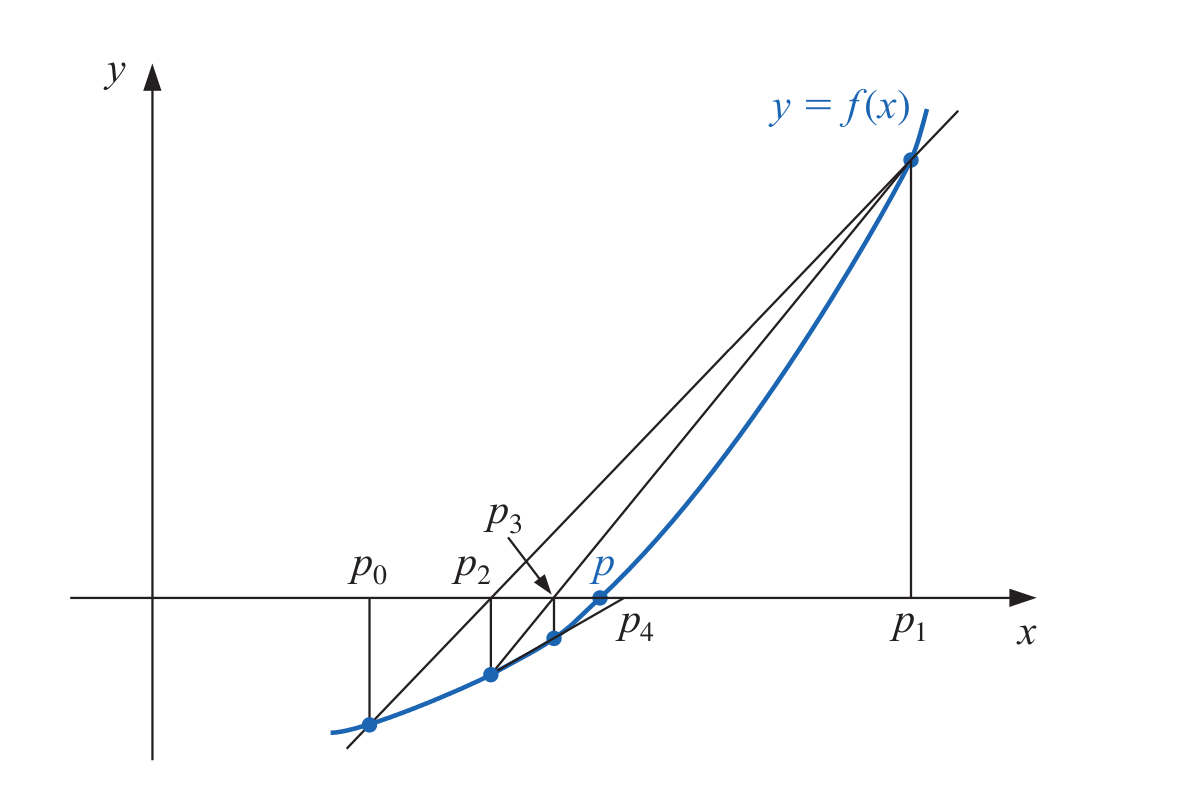
\includegraphics[scale = 0.23]{imagenes/secante.png}~\\[0.25cm]
\end{center}

Explícitamente, la aproximación que estamos usando es

\[f'(x_n) = \frac{f(x_n) - f(x_{n - 1})}{x_n - x_{n - 1}}\]

Por lo tanto, la sucesión que usa este método está dada por

\[x_{n + 1} = x_n - \frac{f(x_n)}{\frac{f(x_n) - f(x_{n - 1})}{x_n - x_{n - 1}}} = x_n - \frac{f(x_n)(x_n - x_{n - 1})}{f(x_n) - f(x_{n - 1})}\]

Se puede demostrar que la velocidad de este método es supralineal.

\subsubsection{Ventajas y desventajas}

\paragraph{Ventajas}
\begin{itemize}
\item No es necesario computar ningún valor de $f'$.
\end{itemize}

\paragraph{Desventajas}
\begin{itemize}
\item La velocidad de convergencia es más lenta que la del método de Newton.

\item A medida que $n$ crece y $x_n$ va convergiendo, $x_n \approx x_{n - 1}$ y $f(x_n) \approx f(x_{n - 1})$, lo que produce una pérdida de dígitos significativos debido al redondeo en el término $\frac{f(x_n)(x_n - x_{n - 1})}{f(x_n) - f(x_{n - 1})}$. El método Regula Falsi provee una solución a este problema.
\end{itemize}

\subsection{Método Regula Falsi}

Genera aproximaciones del mismo modo que el método de la Secante, pero en cada paso verifica que la raíz buscada quede entre dos iteraciones sucesivas, en forma análoga al método de Bisección.

Comienza con dos puntos $x_0$ y $x_1$ tal que $f(x_0)f(x_1) < 0$. Dados $x_{n - 1}$ y $x_n$, el punto $x_{n + 1}$ se calcula mediante la intersección de la recta secante que pasa por $f(x_{n - 1})$ y $f(x_n)$, y el eje $x$. Luego, redefine $x_n$ como aquel valor $x_{n - 1}$ o $x_n$ que tiene distinto signo (evaluado en $f$) que $x_{n + 1}$. La fórmula de la iteración sigue siendo la misma del método de la Secante.

En otras palabras, es idéntico al método de Bisección excepto que, en lugar de quedarse con el punto medio, toma la intersección entre la secante y el eje $x$.

Se puede probar que la velocidad de convergencia del método es al menos $\varphi = \frac{1 + \sqrt{5}}{2}$.

\subsubsection{Ventajas y desventajas}

\paragraph{Ventajas}
\begin{itemize}
\item Desde el punto de vista numérico, ahora $f(x_n)$ y $f(x_{n - 1})$ siempre tendrán distinto signo, con lo cual $f(x_n) - f(x_{n - 1})$ es una resta entre números de distinto signo (podemos pensar que es una suma), evitando una cancelación catastrófica.
\end{itemize}

\paragraph{Desventajas}
\begin{itemize}
\item Requiere más operaciones que el método de la secante.
\end{itemize}
\newpage
\section{Sistemas de ecuaciones lineales}

\subsection{Problema}

Dadas $n$ ecuaciones, cada una con $n$ incógnitas

\[\begin{cases}
a_{11} x_1 + \cdots + a_{1n} x_n = b_1 \\
\hspace{1.45cm}\vdots \\ 
a_{1n} x_1 + \cdots + a_{nn} x_n = b_n 
\end{cases}\]

con coeficientes reales, queremos hallar valores de $x_1, \cdots, x_n$ que satisfagan todas las ecuaciones simultaneamente. En forma matricial escribimos el problema definiendo

\[A = \begin{pmatrix}
a_{11} & \cdots & a_{1n}\\
\vdots & \ddots & \vdots\\
a_{n1} & \cdots & a_{nn}
\end{pmatrix}
\hspace{1cm}
x = \begin{pmatrix}
x_1 \\
\vdots \\
x_n
\end{pmatrix}
\hspace{1cm}
b = \begin{pmatrix}
b_1 \\
\vdots \\
b_n
\end{pmatrix}\]

de modo tal que buscamos soluciones de la ecuación $Ax = b$.

\subsection{Existencia y unicidad de la solución}

Notemos que 

\[
Ax = b \Leftrightarrow x_1 \begin{pmatrix} a_{11}\\ \vdots\\ a_{n1}\end{pmatrix} + \cdots + x_n \begin{pmatrix} a_{1n}\\ \vdots\\ a_{nn}\end{pmatrix} = \begin{pmatrix} b_{1}\\ \vdots\\ b_{n}\end{pmatrix}
\]

En otras palabras, $Ax = b$ tiene solución si y sólo si $b$ es combinación lineal de las columnas de $A$. Usando esto podemos separar en casos:

\begin{itemize}
	\item Si las columnas de $A$ son linealmente independientes, entonces forman una base de $\mathbb{R}^n$ (porque son $n$), y en consecuencia la combinación lineal existe y es única.
	\item Si las columnas de $A$ no son linealmente independientes, entonces una tal combinación lineal puede existir como no. Si existe alguna entonces hay infinitas combinaciones lineales que cumplen la condición.
\end{itemize}

En definitiva $Ax = b$ tiene solución única si y sólo si las columnas de $A$ son l. i. Si no son l. i. entonces hay inifinitas soluciones o no hay ninguna.

\subsection{Resolución de un sistema lineal}

\begin{enumerate}
\item \textbf{Caso $A$ diagonal}. El sistema tiene la forma

\[\begin{cases}
a_{11} x_1 \hspace{2.3cm} = b_1 \\
\hspace{1.35cm}\ddots \\ 
\hspace{2.2cm} a_{nn} x_n = b_n 
\end{cases}\]

Pueden pasar dos cosas:

\begin{itemize}
\item Si $a_{ii} \neq 0$ para todo $i$, entonces la única solución es $x_i = \frac{b_i}{a_{ii}}$, $i = 1, \cdots, n$.
\item Si no, existe $i_0 \in \{1, \cdots, n\}$ tal que $a_{i_0i_0} = 0$. Entonces la ecuación $a_{i_0i_0} x_{i_0} = b_{i_0}$ es equivalente a $b_{i_0} = 0$.
\begin{itemize}
\item Si $b_{i_0} \neq 0$ entonces tenemos una contradicción y el sistema no tiene solución.
\item Si $b_{i_0} = 0$ entonces la ecuación se cumple para cualquier $x_{i_0}$. Si existe solución (depende de lo que suceda con las restantes ecuaciones) entonces habrá infinitas.
\end{itemize}
\end{itemize}

El costo del cómputo en este caso es claramente $\mathcal{O}(n)$.

\item \textbf{Caso $A$ triangular superior}. El sistema tiene la forma

\[\begin{cases}
a_{11} x_1 + a_{12} x_2 + \cdots + a_{1n} x_n = b_1 \\
\hspace{1.26cm} a_{22} x_2 + \cdots + a_{2n} x_n = b_2 \\
\hspace{2.5cm}\vdots \\ 
\hspace{3.35cm} a_{nn} x_n = b_n
\end{cases}\]

Pueden pasar dos cosas:

\begin{itemize}
\item Si $a_{ii} \neq 0$ para todo $i$, entonces las columnas de $A$ son l. i. y la solución es única. Más aún, es

\begin{align}
x_n &= \frac{b_n}{a_{nn}}	\nonumber\\
x_{n - 1} &= \frac{b_{n - 1} - a_{(n-1)n} x_n}{a_{(n-1)(n-1)}}	\nonumber\\
&\vdots \nonumber\\
x_1 &= \frac{b_1 - a_{12}x_2 - a_{13}x_3 - \cdots - a_{1n} x_n}{a_{11}}	\nonumber
\end{align}

Este algoritmo para computar las soluciones de un sistema de ecuaciones triangular superior determinado, recibe el nombre de \textit{backward substitution}. Cuando el sistema es triangular inferior determinado, la sustitución se realiza comenzando desde la primer ecuación, y recibe el nombre de \textit{forward substitution}.

\item Si no, existe $i_0 \in \{1, \cdots, n\}$ tal que $a_{i_0i_0} = 0$. Entonces la ecuación $a_{i_0i_0} x_{i_0} = b_{i_0} - a_{i_0(i_0 + 1)} x_{i_0+1} - \cdots - a_{i_0n} x_n$ es equivalente a $0 = b_{i_0} - a_{i_0(i_0 + 1)} x_{i_0+1} - \cdots - a_{i_0n} x_n$.
\begin{itemize}
\item Si el lado derecho es distinto de 0 entonces tenemos una contradicción y el sistema no tiene solución.
\item Si no, la ecuación se cumple para cualquier $x_{i_0}$. Si existe solución (depende de lo que suceda con las restantes ecuaciones) entonces habrá infinitas.
\end{itemize}


\end{itemize}

El costo del cómputo en este caso es $\mathcal{O}(n^2)$, pues para la incógnita $x_i$ ($i = 1, \cdots, n$) se realizan $\mathcal{O}(n)$ operaciones, y son $n$ incógnitas en total.

\item \textbf{Caso general}. Para resolver el problema para una matriz $A$ cualquiera, la transformaremos mediante operaciones elementales de filas y luego usaremos backward substitution. El algoritmo para transformar el sistema en uno triangular superior se conoce como \textit{eliminación gaussiana}.\\

\end{enumerate}

\subsection{Eliminación gaussiana sin pivoteo}

El algoritmo opera sobre la matriz ampliada del sistema. Llamamos

\[M^{(k)} = \left(\begin{array}{ccc|c}
a_{11}^{(k)} & \cdots & a_{1n}^{(k)} & b_1^{(k)}\\
\vdots & \ddots & \vdots & \vdots\\
a_{n1}^{(k)} & \cdots & a_{nn}^{(k)} & b_n^{(k)}
\end{array}\right)\]

a la matriz ampliada luego de $k$ pasos del algoritmo. Inicialmente, asumamos que $a_{(k+1)(k+1)}^{(k)} \neq 0$ para todo $k$. La entrada es $M^{(0)} = \left(\begin{array}{c|c}A & b\end{array}\right)$. En el primer paso, el algoritmo de eliminación gaussiana fuerza, mediante operaciones de filas, la aparición de ceros en la primer columna, debajo de la diagonal,

\texttt{Paso 1:} $F_i \leftarrow F_i - \frac{a_{i1}^{(0)}}{a_{11}^{(0)}}F_1$ para $i = 2, \cdots, n$

\texttt{Paso 2:} $F_i \leftarrow F_i - \frac{a_{i2}^{(1)}}{a_{22}^{(1)}}F_2$ para $i = 3, \cdots, n$

En el paso $k < n$, colocamos ceros en la columna $k$, debajo de la diagonal,

\texttt{Paso k:} $F_i \leftarrow F_i - \frac{a_{ik}^{(k - 1)}}{a_{kk}^{(k - 1)}}F_k$ para $i = k + 1, \cdots, n$

El último será el

\texttt{Paso n - 1:} $F_i \leftarrow F_i - \frac{a_{i(n-1)}^{(n-2)}}{a_{(n-1)(n-1)}^{(n-2)}}F_{n - 1}$ para $i = n$

El invariante fundamental de este proceso es que al principio del paso $k$, las primeras $k - 1$ columnas tienen únicamente ceros debajo de la diagonal. Al concluir los $n - 1$ pasos obtendremos la matriz $M^{(n - 1)}$ que es triangular superior.
 
\begin{algorithm}
\DontPrintSemicolon
%\SetKwInOut{Input}{input}
%\SetKwInOut{Output}{output}
%\Input{$A \in \mathbb{R}^{n \times n}$ matriz del sistema
%\\$b \in \mathbb{R}^n$ vector de términos independientes}
%\Output{Un sistema equivalente con matriz triangular superior}

\For{$k$ = 1 \KwTo $n - 1$}{
	\For{$i$ = $k + 1$ \KwTo $n$}{
		$m_{ik} = \frac{a_{ik}}{a_{kk}}$\;
		$F_i \leftarrow F_i - m_{ik} F_k$\;
	}
}
\caption[]{Eliminación gaussiana sin pivoteo}
\end{algorithm}

La complejidad del algoritmo es claramente $\mathcal{O}(n^3)$, pues para cada una de las $n$ columnas se hacen $\mathcal{O}(n)$ operaciones de fila, y cada una de estas operaciones de fila son $\mathcal{O}(n)$ operaciones escalares. Un análisis más fino muestra que la cantidad de operaciones de punto flotante que realiza la eliminación gaussiana es aproximadamente $\frac{1}{3}n^3$.

\subsection{Eliminación gaussiana con pivoteo}

Se llama \textit{pivote} al elemento $a^{(k - 1)}_{kk}$ de cada iteración del algoritmo, utilizado para computar los coeficientes $m_{ik}$ e introducir ceros debajo de la diagonal. Puede suceder que al principio de cierto paso de la eliminación gaussiana, digamos el $k$, el elemento $a^{(k - 1)}_{kk}$ sea 0. En este caso no podemos usar $a^{(k-1)}_{kk}$ como pivote. Tenemos dos posibilidades:

\begin{itemize}
\item Si $a^{(k-1)}_{ik} = 0$ para todo $i = k + 1, \cdots, n$, entonces la columna $k$ ya tiene todos ceros debajo de la diagonal, y por lo tanto no es necesario realizar ninguna acción en este paso.
\item Si no, debemos intercambiar la fila $k$ por alguna otra fila $i_0 > k$ tal que $a^{(k-1)}_{i_0k} \neq 0$, y continuar con la eliminación normalmente.
\end{itemize}

Repitiendo esto cada vez que ocurra el problema a lo largo de la ejecución del algoritmo, llegaremos nuevamente a una matriz triangular inferior. 

\begin{obs}{
\label{obs:sistemas1}
Si ahora esas mismas permutaciones de filas fueran realizadas en el mismo orden sobre $A$, entonces se puede probar que la matriz que se obtiene admite eliminación gaussiana sin pivoteo. En términos matriciales, existe una matriz $P \in \mathbb{R}^{n \times n}$ que es producto de matrices elementales de permutación tal que $PA$ admite eliminación gaussiana sin pivoteo.
}\end{obs}

\begin{obs}{
Toda matriz $A \in \mathbb{R}^{n \times n}$ admite eliminación gaussiana con pivoteo, aunque no necesariamente sin pivoteo.
}\end{obs}

\subsection{Pivoteo parcial}

Los coeficientes $m_{ik}$ de cada paso dependen de $a_{ik}^{(k - 1)}$ y $a_{kk}^{(k - 1)}$ que son resultados de operaciones realizadas a lo largo de las iteraciones $1, \cdots, k - 1$ y que, en consecuencia, acarrean un error de redondeo. Si al computar el cociente $\frac{a_{ik}^{(k - 1)}}{a_{kk}^{(k - 1)}}$ resulta que el divisor $a_{kk}^{(k - 1)}$ es un número con valor absoluto pequeño, el error que acumulaba $a_{ik}$ se ve amplificado. Por esta razón, es deseable que $a_{kk}$ tenga valor absoluto lo más grande posible. Con este objetivo se implementa la estrategia de \emph{pivoteo parcial}: al comienzo del $k$-ésimo paso, se permuta la fila $k$ con alguna fila $i_0 \geq k$ tal que $|a_{i_0k}^{(k - 1)}| = \max\limits_{k \leq i \leq n} |a_{ik}^{(k - 1)}|$.

Cuanto mayor sea el pivote, más pequeño será $m_{ik}$ y en consecuencia la operación  $F_i \leftarrow F_i - m_{ik}F_k$ sobre la matriz ampliada del sistema no hará variar sus entradas en gran medida. Intuitivamente, la variación del valor absoluto de los elementos de la matriz ampliada a lo largo de las iteraciones es una medida de la efectividad del pivoteo parcial. En este sentido definimos lo siguiente.

\begin{defi}
Sea $A \in \mathbb{R}^{n \times n}$. Como antes, sea $A^{(k)}$ la matriz ampliada de un sistema que tiene a $A$ como matriz, luego de $k$ pasos de eliminación gaussiana con pivoteo parcial. Sea $a_k = \max\limits_{1 \leq i, j \leq n} |a_{ij}^{(k)}|$. Definimos el factor de crecimiento de $A$ como

\[
\rho = \frac{\max\limits_{1\leq k \leq n - 1}a_k}{a_0}
\]
\end{defi}

Por lo dicho arriba, es conveniente que $\rho$ sea lo más pequeño posible. El siguiente resultado establece una cota para este factor en ciertos tipos de matrices.

\begin{propo} Sea $A \in \mathbb{R}^{n \times n}$.
\begin{itemize}
\item Si $A$ es una matriz arbitraria entonces $\rho \leq 2^{n - 1}$.
\item Si $A$ es una matriz de Hessemberg (sus coeficientes debajo de la primer subdiagonal son nulos) entonces $\rho \leq n$.
\item Si $A$ es una matriz tridiagonal entonces $\rho \leq 2$.
\end{itemize}
\end{propo}

Si bien en una matriz arbitraria el factor de crecimiento es a lo sumo $2^{n - 1}$, este máximo ocurre rara vez y, en general, la estrategia de pivoteo parcial es una estrategia numéricamente estable.

\subsection{Factorización LU}

\begin{defi}
Sea $A \in \mathbb{R}^{n \times n}$. Se llama factorización LU de A a una escritura de la forma $A = LU$ con $L \in \mathbb{R}^{n \times n}$ triangular inferior con unos en la diagonal y $U \in \mathbb{R}^{n \times n}$ triangular superior.
\end{defi}

Veamos cómo calcular la factorización LU de una matriz $A$. Supongamos que $A$ admite eliminación gaussiana sin pivoteo. Notemos que en el paso $k$ de la eliminación se realizan las operaciones de fila $F_i = F_i - m_{ik} F_k$ para $i = k + 1, \cdots, n$. En términos matriciales esto es multiplicar $A^{(k)}$ a izquierda por las matrices de elementales

\[
M_k = 
\begin{pmatrix} 
1 		& \cdots 	& 0 				& \cdots 	& 0 \\
0 		& \ddots 	& 0 				& \cdots 	& 0 \\
\vdots 	& 			& 1 				& 			& \vdots\\
0		& \cdots		& -m_{(k+1)k} 	& \cdots		& 0\\
\vdots	& 			& \vdots		 	& \ddots		& \vdots\\
0		& \cdots		& 0				& \cdots		& 1\\
\end{pmatrix}
\cdots
\begin{pmatrix} 
1 		& \cdots 	& 0 				& \cdots 	& 0 \\
0 		& \ddots 	& 0 				& \cdots 	& 0 \\
\vdots 	& 			& 1 				& 			& \vdots\\
0		& \cdots		& 0 	& \cdots		& 0\\
\vdots	& 			& \vdots		 	& \ddots		& \vdots\\
0		& \cdots		& -m_{nk}	& \cdots		& 1\\
\end{pmatrix}
=
\begin{pmatrix} 
1 		& \cdots 	& 0 				& \cdots 	& 0 \\
0 		& \ddots 	& 0 				& \cdots 	& 0 \\
\vdots 	& 			& 1 				& 			& \vdots\\
0		& \cdots		& -m_{(k+1)k} 	& \cdots		& 0\\
\vdots	& 			& \vdots		 	& \ddots		& \vdots\\
0		& \cdots		& -m_{nk}	& \cdots		& 1\\
\end{pmatrix}
\]

Al cabo de los $n - 1$ pasos de eliminación gaussiana tendremos que $M_{n - 1} \cdots M_1 A = U$ con $U$ triangular superior. 

Observemos que $M_k$ es inversible para cada $k$, puesto que $M_k$ es triangular inferior con unos en la diagonal. Entonces podemos escribir $A = M_1^{-1}\cdots M_{n - 1}^{-1} U = LU$, con $L = M_1^{-1}\cdots M_{n - 1}^{-1}$. Si bien ya hemos llegado a la factorización LU de $A$, podemos simplificar la expresión de $L$. Notemos que $M_k = I_n - m_k e_k^t$ con $m_k = \begin{pmatrix}0\\ \vdots \\ 0 \\ m_{(k+1)k} \\ \vdots \\ m_{nk}\end{pmatrix}$ y $e_k$ el $k$-ésimo vector canónico de $\mathbb{R}^n$. Usando esta escritura es fácil ver que $M_k^{-1} = I_n + m_k e_k^t$, ya que

\begin{align*}
(I_n - m_k e_k^t)(I_n + m_k e_k^t) & = I_n^2 + m_k e_k^t - m_k e_k^t - m_k e_k^t m_k e_k^t &\\
& = I_n^2 - m_k e_k^t m_k e_k^t &\\
& = I_n & \text{(pues } e_k^t m_k = 0\text{)}
\end{align*}

Luego,

\begin{align*}
L & = M_1^{-1} \cdots M_{n - 1}^{-1} &\\
	& = (I_n + m_1 e_1^t) \cdots (I_n + m_{n - 1} e_{n - 1}^t) &\\
	& = I_n + m_1 e_1^t + \cdots + m_{n - 1} e_{n - 1}^t & \text{(pues } e_i^t m_j = 0 \text{ si } i \leq j \text{)}
\end{align*}

En definitiva $A = LU$ con $L = \begin{pmatrix} 
1 			& \cdots 	& 0 				& \cdots 	& 0 \\
m_{21} 		& \ddots 	& 0 				& \cdots 	& 0 \\
\vdots 		& 			& 1 				& 			& \vdots\\
m_{(k+1)1}	& \cdots		& m_{(k+1)k} 	& \cdots		& 0\\
\vdots		& 			& \vdots		 	& \ddots		& \vdots\\
m_{n1}		& \cdots		& m_{nk}		& \cdots		& 1\\
\end{pmatrix}$.

Debido a lo inherente que es la factorización LU al proceso de eliminación gaussiana el costo de computar esta factorización es claramente $\mathcal{O}(n^3)$.

\subsubsection{Existencia y unicidad de la factorización LU}

Hemos probado lo siguiente,

\begin{propo}
Sea $A \in \mathbb{R}^{n \times n}$. Si $A$ admite eliminación gaussiana sin pivoteo entonces $A$ tiene factorización LU.
\end{propo}

\begin{obs}
La recíproca no es cierta. Por ejemplo, la matriz nula tiene factorización LU pero obviamente no admite eliminación gaussiana sin pivoteo.
\end{obs}

\begin{obs}
No toda matriz tiene factorización LU. Si $A \in \mathbb{R}^{2 \times 2}$ tiene factorización LU entonces existen $a, b, c, d \in \mathbb{R}$ tal que

\[A = \begin{pmatrix}1 & 0\\a & 1\end{pmatrix} \begin{pmatrix}b & c\\0 & d\end{pmatrix} = \begin{pmatrix}
b & c\\ab & ac + d
\end{pmatrix}\]

Teniendo en cuenta esta condición necesaria, es fácil ver que la matriz $\begin{pmatrix}
0 & 0\\1 & 0
\end{pmatrix}$ no tiene factorización LU.

\end{obs}

\begin{obs}
Remitiéndonos a la Observación \ref{obs:sistemas1}, deducimos que existe $P \in \mathbb{R}^{n \times n}$ producto de matrices de permutación tal que $PA$ tiene factorización LU. Pero $P$ es producto de matrices inversibles, con lo cual existe $P^{-1}$, y llegamos a la escritura $A = P^{-1}LU$, que se llama factorización PLU. Observemos que como una tal matriz $P$ siempre existe entonces también existirá siempre una factorización PLU.
\end{obs}

Con respecto a la unicidad, se tiene el siguiente resultado,

\begin{propo}
Sea $A \in \mathbb{R}^{n \times n}$ inversible. Si $A$ tiene factorización LU entonces dicha escritura es única.

\begin{proof}
Sean $A = L_1 U_1 = L_2 U_2$ dos escrituras LU de $A$. Como $A$, $L_1$ y $L_2$ son inversibles, entonces $U_1$ y $U_2$ también lo son. Luego $L_1 U_1 = L_2 U_2 \Rightarrow U_1 U_2^{-1} = L_1^{-1} L_2$. Como $U_2$ es triangular superior entonces $U_2^{-1}$ también lo es. Como producto de matrices triangulares superiores es triangular superior, entonces $U_1 U_2^{-1}$ es triangular superior. Análogamente $L_1^{-1} L_2$ resulta triangular inferior. Sin embargo este último producto tiene una característica distintiva. Como $L_1$ tiene unos en la diagonal, $L_1^{-1}$ los preserva, y como $L_2$ también tiene unos en la diagonal, entonces el producto $L_1^{-1} L_2$ también tiene unos en la diagonal.

Entonces $U_1 U_2^{-1} = L_1^{-1} L_2$, siendo $U_1 U_2^{-1}$ triangular superior y $L_1^{-1} L_2$ triangular inferior. Luego, ambos productos deben ser una matriz diagonal. Más aún, como $L_1^{-1} L_2$ tiene unos en la diagonal, entonces esta matriz diagonal es la identidad. Finalmente, $U_1 U_2^{-1} = I_n \Rightarrow U_1 = U_2$ y $L_1^{-1}L_2 = I_n \Rightarrow L_1 = L_2$, es decir, las escrituras son idénticas.

\end{proof}
\end{propo}

\begin{obs}
En general, la factorización LU de una matriz no es única. Por ejemplo, la matriz nula admite infinitas factorizaciones LU.
\end{obs}

\subsubsection{Aplicación}
Supongamos que dada una matriz $A$ con factorización LU y vectores $b_1, \cdots, b_k$ queremos calcular una solución de $Ax = b_i$ para cada $i = 1, \cdots, k$. Si usáramos el algoritmo de eliminación gaussiana junto con backward substitution para resolver cada uno de los sistemas, tendríamos un costo de $\mathcal{O}(n^3)$ por cada sistema.

Por otro lado, factoricemos $A = LU$. Esta escritura se puede calcular, como dijimos antes, en $\mathcal{O}(n^3)$. Para cada sistema $Ax = b_i$ hacemos:
\begin{itemize}
\item Calculamos una solución de $Ly = b_i$, mediante forward substitution.
\item Calculamos una solución de $Ux = y$, mediante backward substitution.
\end{itemize}

Esto requiere tiempo $\mathcal{O}(n^2)$. Notemos que como $L$ es inversible, $Ux = y \Leftrightarrow LUx = Ly \Leftrightarrow Ax = b_i$. En definitiva, podemos resolver $Ax = b_i$ en $\mathcal{O}(n^2)$, para cada $i$, pagando una única vez, inicialmente, un costo de $\mathcal{O}(n^3)$.

\subsubsection{Familias de matrices que admiten factorización LU}

\begin{defi}
Una matriz $A \in \mathbb{R}^{n \times n}$ se dice estrictamente diagonal dominante por filas si

\[
|a_{ii}| > \sum_{\substack{j = 1\\ j \neq i}}^n |a_{ij}|
\]

para todo $i = 1, \cdots, n$.
\end{defi}

\begin{propo}
Si $A \in \mathbb{R}^{n \times n}$ es e. d. d. f. entonces $A$ admite factorización LU.

\begin{proof}
Lo probamos por inducción en $n \in \mathbb{N}$. Escribamos $A = (a_{ij})_{i, j}$.

Si $n = 1$ la factorización es trivial.

Sea $n > 1$. Escribimos la matriz $A$ por bloques en la forma

\[A = \left(\begin{array}{c|c}
a_{11} & v^t\\ \hline
u & A_{n - 1}
\end{array}\right)\]

donde $u = \begin{pmatrix}a_{21} \\ \vdots \\ a_{n1} \end{pmatrix}$, $v^t = (a_{12} \text{ } \cdots \text{ } a_{1n})$ y $A_{n - 1}$ es la submatriz que se obtiene sacandole la primera fila y columna a $A$. Como $a_{11} \neq 0$, podemos aplicar el primer paso de eliminación gaussiana sin pivoteo,

\[\left(\begin{array}{c|c}
1 & 0 \cdots 0\\ \hline
-u / a_{11} & I_{n - 1} 
\end{array}\right)
\left(\begin{array}{c|c}
a_{11} & v^t\\ \hline
u & A_{n - 1}
\end{array}\right) =
\left(\begin{array}{c|c}
a_{11} & v^t\\ \hline
0 & \\
\vdots & -uv^t / a_{11} + A_{n - 1}\\
0 & 
\end{array}\right)\]

Veamos que el bloque $B = -uv^t / a_{11} + A_{n - 1}$ es una matriz e. d. d. f. Por comodidad supondremos que los índices de las matrices de dimensión $(n - 1) \times (n - 1)$ que estamos considerando corren de 2 hasta $n$. Si $2 \leq i, j \leq n$ son cualesquiera entonces

\begin{align*}
B_{ij} & = (-uv^t / a_{11} + A_{n - 1})_{ij} \\
& = (-uv^t / a_{11})_{ij} + (A_{n - 1})_{ij}\\
& = -1 / a_{11} (uv^t)_{ij} + a_{ij}\\
& = a_{ij} - \frac{a_{i1}a_{1j}}{a_{11}}
\end{align*}

Luego,

\begin{align*}
\sum_{\substack{j = 2\\ j \neq i}}^n |B_{ij}| & = \sum_{\substack{j = 2\\ j \neq i}}^n \left|a_{ij} - \frac{a_{i1}a_{1j}}{a_{11}}\right|\\
& \leq \sum_{\substack{j = 2\\ j \neq i}}^n |a_{ij}| + \sum_{\substack{j = 2\\ j \neq i}}^n \left|\frac{a_{i1}a_{1j}}{a_{11}}\right|\\
& = \sum_{\substack{j = 2\\ j \neq i}}^n |a_{ij}| + \left|\frac{a_{i1}}{a_{11}}\right| \sum_{\substack{j = 2\\ j \neq i}}^n \left|a_{1j}\right|\\
\end{align*}

Pero $\sum_{\substack{j = 2\\ j \neq i}}^n |a_{ij}| = \sum_{\substack{j = 1\\ j \neq i}}^n |a_{ij}| - |a_{i1}| < |a_{ii}| - |a_{i1}|$, esto último por ser $A$ estrictamente diagonal dominante por filas. Por la misma razón se tiene $\sum_{\substack{j = 2\\ j \neq i}}^n |a_{1j}| = \sum_{j = 2}^n |a_{1j}| - |a_{1i}| < |a_{11}| - |a_{1i}|$. Entonces,

\begin{align*}
\sum_{\substack{j = 2\\ j \neq i}}^n |B_{ij}| & < |a_{ii}| - |a_{i1}| + \left|\frac{a_{i1}}{a_{11}}\right|(|a_{11}| - |a_{1i}|)\\
& = |a_{ii}| - |a_{i1}| + |a_{i1}| - \left|\frac{a_{i1} a_{1i}}{a_{11}}\right|\\
& = |a_{ii}| - \left|\frac{a_{i1} a_{1i}}{a_{11}}\right|
\end{align*}

Finalmente, como $|a_{ii}| - \left|\frac{a_{i1} a_{1i}}{a_{11}}\right| \leq \left|a_{ii} - \frac{a_{i1} a_{1i}}{a_{11}}\right|$,

\[\sum_{\substack{j = 2\\ j \neq i}}^n |B_{ij}| < \left|a_{ii} - \frac{a_{i1} a_{1i}}{a_{11}}\right|\\
= |B_{ii}|\]
Que es lo que queríamos probar. Entonces, por hipótesis inductiva, $B$ admite factorización LU. Sea $B = L_{n - 1} U_{n - 1}$ una tal escritura. Sean

\[L = \left(\begin{array}{c|c}
1 & 0 \cdots 0\\ \hline
v / a_{11} & L_{n - 1} 
\end{array}\right)
\hspace{0.5cm}
U = \left(\begin{array}{c|c}
a_{11} & u^t\\ \hline
0 & \\
\vdots & U_{n - 1}\\
0 &
\end{array}\right)
\]

Notemos que $L$ es triangular inferior con unos en la diagonal y $U$ es triangular superior. Se puede ver, haciendo el producto por bloques, que $A = LU$, con lo cual esta es la factorización LU de $A$. Esto concluye el paso inductivo.

\end{proof}
\end{propo}

\begin{propo}
\label{propo:lu}

Sea $A \in \mathbb{R}^{n \times n}$ inversible. Entonces $A$ tiene factorización LU si y sólo si sus $n$ menores principales son no nulos.

\begin{proof}
Denotamos $A_i$ a la submatriz de $A$ formada por las primeras $i$ filas e $i$ columnas.\\[0.25cm]
($\Rightarrow$) Queremos ver que $\det(A_i) \neq 0$ para todo $i = 1, \cdots, n$. Procedemos por inducción en $n \in \mathbb{N}$.

Si $n = 1$ entonces $A = \begin{pmatrix} a \end{pmatrix}$ para cierto $a \in \mathbb{R}$, que es no nulo puesto que $A$ es inversible. Entonces $\det(A) = \det(A_1) \neq 0$.

Sea $n > 1$. Como $A$ es inversible entonces $\det(A) = \det(A_n) \neq 0$. Sea $A = LU$ una factorización LU de $A$. Descomponemos a $L$ y $U$ en bloques del siguiente modo,

\[L = \left(\begin{array}{c|c}
 & 0 \\
L_{n - 1} & \vdots \\
 & 0 \\ \hline
v^t & 1
\end{array}\right)
\hspace{0.5cm}
U = \left(\begin{array}{c|c}
 &  \\
U_{n - 1} & u \\
 &  \\ \hline
0 \cdots 0 & x
\end{array}\right)
\]

con $L_{n - 1}, U_{n - 1} \in \mathbb{R}^{(n - 1) \times (n - 1)}$, $v, u \in \mathbb{R}^{n - 1}$ y $x \in \mathbb{R}$. Entonces

\[A = LU = \left(\begin{array}{c|c}
L_{n - 1} U_{n - 1} & L_{n - 1}u\\ \hline
v^t U_{n - 1} & v^tu + x
\end{array}\right)\]

Por lo tanto $A_{n - 1} = L_{n - 1}U_{n - 1}$, es decir que esta submatriz tiene factorización LU. Veamos que, además, es inversible. Por un lado, como $L_{n - 1}$ es triangular inferior con unos en la diagonal, entonces es inversible. Por otro lado, como $A$ y $L$ son inversibles, entonces $U$ es inversible. Luego $0 \neq \det U = \det(U_{n - 1}) \det(x)$, con lo cual $\det(U_{n - 1}) \neq 0$, es decir, $U_{n - 1}$ es inversible. Por ende $L_{n - 1}$ y $U_{n - 1}$ son inversibles, y en consecuencia $A_{n - 1}$ también lo es.

Todo esto hace que valga la hipótesis inductiva sobre $A_{n - 1}$, y por lo tanto sus $n - 1$ menores principales son no nulos. Pero estos menores principales son exactamente $\det(A_1), \cdots, \det(A_{n - 1})$.\\[0.25cm]

($\Leftarrow$) Inducción en $n \in \mathbb{N}$.

Si $n = 1$ la factorización LU de $A$ es trivial.

Sea $n > 1$. Por hipótesis, la submatriz $A_{n - 1}$ tiene todos sus menores principales no nulos. Entonces, por hipótesis inductiva, admite una factorización LU que la escribimos $A_{n - 1} = L_{n - 1}U_{n - 1}$. Descomponemos $A$ en bloques del siguiente modo

\[A = \left(\begin{array}{c|c}
L_{n - 1} U_{n - 1} & u\\ \hline
v^t & a
\end{array}\right)\]

Definimos los vectores $\alpha, \beta \in \mathbb{R}^{n - 1}$ como

\[\alpha = (L_{n - 1})^{-1}u\]
\[\beta = (U_{n - 1}^t)^{-1} v\]

Esto es posible gracias a que las dimensiones son adecuadas y las matrices $L_{n - 1}$ y $U_{n - 1}^t$ son inversibles, por ser $A_{n - 1}$ inversible. Finalmente definimos el número real

\[x = a - \beta^t \alpha\]

A partir de estos elementos vamos a obtener la factorización LU de $A$. Sean

\[
L = \left(\begin{array}{c|c}
 & 0 \\
L_{n - 1} & \vdots \\
 & 0 \\ \hline
\beta^t & 1
\end{array}\right)
\hspace{0.5cm}
U = \left(\begin{array}{c|c}
 &  \\
U_{n - 1} & \alpha \\
 &  \\ \hline
0 \cdots 0 & x
\end{array}\right)\]

Haciendo la multiplicación es fácil ver que $A = LU$, que es lo que queríamos probar.

\end{proof}
\end{propo}

\subsection{Matrices simétricas definidas positivas y factorización de Cholesky}

\subsubsection{Matrices simétricas y definidas positivas}

\begin{defi}
Una matriz $A \in \mathbb{R}^{n \times n}$ se dice definida positiva si $x^tAx > 0$ para todo $x \neq 0$.
\end{defi}

\begin{propo}
Si $A \in \mathbb{R}^{n \times n}$ es definida positiva entonces es inversible.

\begin{proof}
Veamos el contrarrecíproco. Si $A$ no es inversible entonces existe $x \in \mathbb{R}^n$ no nulo tal que $Ax = 0$. Entonces $x^t A x = 0$, y como $x \neq 0$ esto implica que $A$ no es definida positiva.
\end{proof}
\end{propo}

\begin{propo}
\label{propo:defpos}
Si $A \in \mathbb{R}^{n \times n}$ es definida positiva entonces sus submatrices principales son definidas positivas e inversibles.

\begin{proof}
Sea $1 \leq k \leq n$ cualquiera. Sea $A_k$ la submatriz $A$ formada por sus primeras $k$ filas y $k$ columnas, queremos ver que $A_k$ es definida positiva e inversible. Si $k = n$ no hay nada que ver. Supongamos $k < n$. Sea $x_k \in \mathbb{R}^k$ no nulo. A partir de este vector construimos un nuevo vector $x \in \mathbb{R}^n$ agregando ceros, es decir,

\[x = \begin{pmatrix}
x_k\\
0 \\
\vdots \\
0
\end{pmatrix}\]

Multiplicando por bloques se puede ver que $x^t A x = x_k^t A x_k$. Como $x_k \neq 0$ entonces $x \neq 0$, y como $A$ es definida positiva entonces $x^t A x > 0$. Luego $x_k^t A_k x_k > 0$. Dado que $x_k$ es cualquiera, concluimos que $A_k$ es definida positiva, como queríamos.

La inversibilidad de $A_k$ se deduce inmediatamente de la proposición anterior.

\end{proof}
\end{propo}

\begin{coro}
Si $A \in \mathbb{R}^{n \times n}$ es definida positiva entonces admite factorización LU y es única.
\begin{proof}
Por la última proposición, todas las submatrices principales son inversibles. Pero vimos que toda matriz que cumple esto, admite factorización LU. Además por ser $A$ inversible, la escritura es única.
\end{proof}
\end{coro}

\begin{defi}
Una matriz $A \in \mathbb{R}^{n \times n}$ se dice simétrica si $A = A^t$.
\end{defi}

\begin{propo}
\label{propo:ldl}
Sea $A \in \mathbb{R}^{n \times n}$ inversible y simétrica, que admite factorización LU. Entonces existen matrices $L \in \mathbb{R}^{n \times n}$ triangular inferior con unos en la diagonal y $D \in \mathbb{R}^{n \times n}$ diagonal tal que $A = LDL^t$. Esta escritura se conoce como \textit{factorización LDL}.

\begin{proof}
Sea $A = LU$ una factorización LU. Como $A$ es simétrica entonces $A = A^t \Rightarrow LU = (LU)^t = U^t L^t$. Por definición $L$ es inversible. Como $A$ es inversible, $U$ resulta inversible. Entonces $(U^t)^{-1}L = L^t U^{-1}$. Como $U$ es triangular superior, entonces $U^t$ es triangular inferior y $(U^t)^{-1}$ también. Análogamente, como $L$ es triangular inferior, $L^t$ es triangular superior. Además $U^{-1}$ es triangular superior. Luego $(U^t)^{-1}L$ es triangular inferior y $L^t U^{-1}$ es triangular superior, con lo cual ambas matrices resultan ser diagonales. Sea $L^t U^{-1} = D$ diagonal. Como $L^t$ y $U^{-1}$ son inversibles, entonces $D$ también lo es. Luego $D^{-1}L^t = U$, y reemplazando en la factorización original queda $A = LU = LD^{-1}L^t$. Como $D^{-1}$ también es diagonal, esta es la escritura buscada.
\end{proof}
\end{propo}

\begin{coro}
\label{coro:ldl}
Si $A \in \mathbb{R}^{n \times n}$ es simétrica y tiene todos sus menores principales no nulos, entonces admite factorización LDL.

\begin{proof}
Por la Proposición \ref{propo:lu}, $A$ admite factorización LU. Además es inversible. Luego, por la Proposición \ref{propo:ldl}, $A$ admite factorización LDL.
\end{proof}
\end{coro}

\subsubsection{Factorización de Cholesky}

\begin{defi}
Sea $A \in \mathbb{R}^{n \times n}$. Se llama factorización de Cholesky de $A$ a una escritura de la forma $A = LL^t$ con $L$ una matriz triangular inferior con elementos en la diagonal positivos.
\end{defi}

\begin{propo}
Sea $A \in \mathbb{R}^{n \times n}$. Entonces $A$ es simétrica definida positiva si y sólo si admite factorización de Cholesky.

\begin{proof}
($\Rightarrow$) Como $A$ es definida positiva entonces, por la Proposición \ref{propo:defpos}, todos los menores principales de $A$ son no nulos. Como además $A$ es simétrica, por el Corolario \ref{coro:ldl}, $A$ tiene factorización LDL. Sea $A = LDL^t$ una tal escritura.

Veamos que todos los elementos de la diagonal de $D$ son positivos. Sea $1 \leq i \leq n$ arbitrario. Como $L^t$ es inversible, existe $x \in \mathbb{R}^n$ tal que $L^tx = e_i$, y que necesariamente es no nulo. Como $x \neq 0$ entonces $x^t A x > 0$. Luego

\[0 < x^t A x = x^t (LDL^t) x = (x^tL) D (L^tx) = e_i^t D e_i = D_{ii}\]

En definitiva $D_{ii} > 0$ y como $i$ es cualquiera, todos los elementos de la diagonal de $D$ son positivos. Definimos

\[\sqrt{D} = \begin{pmatrix}
\sqrt{D_{11}} & & 0\\
 & \ddots & \\
0 & & \sqrt{D_{nn}}
\end{pmatrix}\]

Notemos que $D = \sqrt{D} \sqrt{D}$, con lo cual $A = LDL^t = L\sqrt{D}\sqrt{D}L^t = L\sqrt{D}\sqrt{D}^tL^t = (L \sqrt{D}) (L \sqrt{D})^t$. Pero $L \sqrt{D}$ sigue siendo triangular inferior y, más aún, los elementos de su diagonal son positivos, pues tanto los de $L$ como los de $\sqrt{D}$ lo son. Así llegamos a la factorización deseada.\\[0.25cm]

($\Leftarrow$) Sea $A = LL^t$ una factorización de Cholesky. Sea $x \neq 0$, queremos ver que $x^t A x > 0$. Se tiene que $x^t A x = x^t LL^t x = (L^tx)^t(L^tx) = \norm{L^tx}_2^2$ y esta norma es estrictamente mayor que cero, ya que como $L^t$ es triangular con diagonal no nula y $x$ es no nulo, entonces $L^tx \neq 0$.

\end{proof}
\end{propo}

Supongamos que $A$ tiene factorización de Cholesky, de modo tal que podemos escribir

\[
A = \begin{pmatrix}
a_{11} & \cdots & a_{n1} \\
\vdots & \ddots & \vdots \\
a_{n1} & \cdots & a_{nn}
\end{pmatrix} = 
\begin{pmatrix}
\ell_{11} & 0 & \cdots & 0 \\
\ell_{21} & \ell_{22} & \cdots & 0 \\
\vdots & \vdots & \ddots & \vdots \\
\ell_{n1} & \ell_{n2} & \cdots & \ell_{nn}
\end{pmatrix}
\begin{pmatrix}
\ell_{11} 	& \ell_{21}	& \cdots & \ell_{n1} \\
0		 	& \ell_{22} 	& \cdots & \ell_{n2} \\
\vdots 		& \vdots 	& \ddots & \vdots \\
0		 	& 0			& \cdots & \ell_{nn}
\end{pmatrix} = LL^t
\]

con $\ell_{ii} > 0$ para todo $i$. Para calcular el coeficiente de la fila $i$ y columna $j$ ($j \leq i$), computamos el producto de la fila $i$ de $L$ contra la columna $j$ de $L^t$:

\[a_{ij} = \begin{pmatrix}
\ell_{i1} & \cdots & \ell_{ij} & \cdots & \ell_{ii} & 0 & \cdots & 0
\end{pmatrix}
\begin{pmatrix}
\ell_{j1} \\
\vdots \\
\ell_{jj} \\
0 \\
\vdots \\
0
\end{pmatrix} = \ell_{i1}\ell_{j1} + \cdots + \ell_{ij}\ell_{jj} = \sum_{k = 1}^j \ell_{ik}\ell_{jk}\]

Usando esta ecuación se deduce que:

\begin{itemize}
\item Si $j = i = 1$ entonces

\[a_{11} = \ell_{11}^2 \Leftrightarrow \ell_{11} = \sqrt{a_{11}}\]

\item Si $j = 1 < i$ entonces

\[a_{i1} = \ell_{i1}\ell_{11} \Leftrightarrow \ell_{i1} = \frac{a_{i1}}{\ell_{11}}\]

\item Si $1 < j = i$ entonces

\[a_{jj} = \ell_{j1}^2 + \cdots + \ell_{jj}^2 \Leftrightarrow \ell_{jj} = \sqrt{a_{jj} - \sum_{k = 1}^{j - 1}\ell_{jk}^2}\]

\item Si $1 < j < i$ entonces

\[a_{ij} = \ell_{i1}\ell_{j1} + \cdots + \ell_{ij}\ell_{jj} \Leftrightarrow \ell_{ij} = \frac{1}{\ell_{jj}}\left(a_{ij} - \sum_{k = 1}^{j - 1}\ell_{ik}\ell_{jk}\right)\]

\end{itemize}

Para calcular cada una de las entradas de la descomposición procedemos por columnas, primero calculando los coeficientes $\ell_{i1}$, luego los $\ell_{i2}$ y así sucesivamente. Se puede ver que de esta forma respetamos las dependencias entre las ecuaciones anteriores.

Esto nos da un algoritmo para computar la matriz $L$ de la factorización. Más aún, como cada $\ell_{ij}$ está unívocamente determinado, hemos probado que la factorización de Cholesky es única.

\begin{algorithm}
\caption[]{Factorización de Cholesky}
$\ell_{11} = \sqrt{a_{11}}$;\\
\For{$i = 2$ to $n$}{
	$\ell_{i1} = \frac{a_{i1}}{\ell_{11}}$;\\
}
\For{$j = 2$ to $n$}{
	$\ell_{jj} = \sqrt{a_{jj} - \sum_{k = 1}^{j - 1}\ell_{jk}^2}$;\\
	\For{$i = j + 1$ to $n$}{
		$\ell_{ij} = \frac{1}{\ell_{jj}}\left(a_{ij} - \sum_{k = 1}^{j - 1}\ell_{ik}\ell_{jk}\right)$;\\
	}
}
\end{algorithm}

La complejidad del algoritmo es cúbica, que es la misma que la de LU. Sin embargo, en términos prácticos el cómputo de la factorización de Cholesky resulta ser el doble de rápido que el de LU. Además, al igual que LU, permite resolver eficientemente el problema de la resolución sucesiva de sistemas de misma matriz $A$.

\subsection{Estabilidad numérica de Cholesky}
A diferencia de LU, Cholesky no depende de pivoteos, manteniendo así el error acotado. El único problema que puede sufrir esta escritura es la presencia del cómputo de raíces cuadradas. Si bien los números a los que se les toma raíz son siempre positivos, si éstos son suficientemente pequeños se pueden tornar negativos a lo largo del cómputo, debido al error de redondeo, siendo imposible continuar con el algoritmo. Pese a que ésto sólo sucede en matrices muy mal condicionadas, para evitarlo puede optarse por sumarle a la matriz $A$ otra matriz diagonal con entradas de valor absoluto chico, y así reforzar su condición de definida positiva. La desventaja en este caso es que se pierde precisión en el resultado.

\newpage
\section{Factorización QR}

\subsection{Matrices ortogonales}

\begin{defi}
Una matriz $Q \in \mathbb{R}^{n \times n}$ se dice ortogonal si $Q^{-1} = Q^t$.
\end{defi}

\begin{obs}
Si $Q$ es ortogonal entonces $Q^t = Q^{-1}$ también, pues $((Q^t)^{-1})^t = ((Q^t)^t)^{-1} = Q^{-1} = Q^t$.
\end{obs}

En lo que sigue, $Q$ es una matriz ortogonal de $n \times n$.

\begin{lema}
$Q$ preserva norma 2, i. e., $\norm{Qx}_2 = \norm{x}_2$.
\end{lema}

\begin{lema}
$\norm{Q}_2 = 1$.
\end{lema}

\begin{coro}
$\kappa_2(Q) = 1$.
\end{coro}

Esto nos dice que las matrices ortogonales son estables, lo cual se condice con el hecho de que preservan norma 2, es decir, que no deforman vectores, haciendo que el error de las componentes escalares no sea amplificado. Este motivo hace a las matrices ortogonales atractivas desde el punto de vista numérico. Además, el cómputo de su inversa no requiere más que una transposición de elementos, y por lo tanto no introduce error.

\begin{defi}
Sea $A \in \mathbb{R}^{n \times n}$. Se llama factorización QR de $A$ a una escritura de la forma $A = QR$ con $Q \in \mathbb{R}^{n \times n}$ una matriz ortogonal y $R \in \mathbb{R}^{n \times n}$ triangular superior. 
\end{defi}

Notemos que de tener la factorización QR, tenemos la cadena de equivalencias $Ax = b \Leftrightarrow QR x = b \Leftrightarrow Rx = Q^t b$ y este último sistema se puede resolver mediante backward substitution, con error mínimo.

\subsection{Método de rotaciones (Givens)}

Dado $\theta \in [0, \frac{\pi}{2}]$ queremos encontrar una transformación lineal $W : \mathbb{R}^2 \to \mathbb{R}^2$ que rote en un ángulo $\theta$ todo vector en el plano. Es fácil ver en forma geométrica que $W$ actúa del siguiente modo sobre la base canónica,

\[W\begin{pmatrix}1 \\ 0\end{pmatrix} = \begin{pmatrix}\cos\theta \\ -\sin \theta\end{pmatrix}\]
\[W\begin{pmatrix}0 \\ 1\end{pmatrix} = \begin{pmatrix}\sin\theta \\ \cos \theta\end{pmatrix}\]

Entonces

\[W = \begin{pmatrix}
\cos \theta & \sin \theta \\
-\sin \theta & \cos \theta
\end{pmatrix}\]

Se puede probar que esto vale para cualquier $\theta \in \mathbb{R}$ (separando en casos, según el cuadrante en que se encuentre $\theta$). De este modo quedan caracterizadas todas las rotaciones en $\mathbb{R}^2$. Notemos que $W$ es ortogonal.

Supongamos que dado $v = \begin{pmatrix}v_1 \\ v_2 \end{pmatrix} \in \mathbb{R}^2$ no nulo, queremos encontrar una rotación $W : \mathbb{R}^2 \to \mathbb{R}^2$ que rote $v$ sobre el eje positivo de las abscisas, es decir, tal que $Wv = \begin{pmatrix}\norm{v}_2 \\ 0\end{pmatrix}$. Usando la forma de una rotación en $\mathbb{R}^2$, tenemos que

\[Wv = \begin{pmatrix}\norm{v}_2 \\ 0\end{pmatrix} \Leftrightarrow 
\begin{pmatrix}
\cos \theta & \sin \theta \\
-\sin \theta & \cos \theta
\end{pmatrix} \begin{pmatrix}v_1 \\ v_2\end{pmatrix} = 
\begin{pmatrix}\norm{v}_2 \\ 0\end{pmatrix} \Leftrightarrow 
\begin{cases}
v_1 \cos \theta  + v_2 \sin \theta  = \norm{v}_2 \\
-v_1 \sin \theta  + v_2 \cos \theta  = 0
\end{cases}\] 

Tomemos $\theta$ tal que $\cos \theta = \frac{v_1}{\norm{v}_2}$ y  $\sin \theta = \frac{v_2}{\norm{v}_2}$. Este $\theta$ existe y es único ($\cos \theta$ y $\sin \theta$ se pueden pensar como las coordenadas $x$ e $y$ respectivamente de un punto sobre la circunferencia unitaria), y se puede verificar que así tomado satisface las ecuaciones previas. De este modo, hemos probado lo siguiente,

\begin{propo}
Sea $v = \begin{pmatrix}v_1 \\ v_2 \end{pmatrix} \in \mathbb{R}^2$ un vector no nulo. La única rotación $W : \mathbb{R}^2 \to \mathbb{R}^2$ que cumple $Wv = \begin{pmatrix}\norm{v}_2 \\ 0 \end{pmatrix}$ es

\[W = \begin{pmatrix}
\frac{v_1}{\norm{v}_2} & \frac{v_2}{\norm{v}_2}\\
-\frac{v_2}{\norm{v}_2} & \frac{v_1}{\norm{v}_2}
\end{pmatrix}\]
\end{propo}

Sea ahora $A = \begin{pmatrix}
a_{11} & a_{12}\\
a_{21} & a_{22}
\end{pmatrix}$ cualquiera y pongamos $v = \begin{pmatrix}a_{11} \\ a_{21}\end{pmatrix}$. Si $v = 0$ entonces $A$ es triangular superior y por lo tanto $I_2 A$ es una factorización QR de $A$. Si $v \neq 0$ construimos, usando la proposición anterior, una rotación $W$ tal que $Wv = \begin{pmatrix}\norm{v}_2 \\ 0\end{pmatrix}$, con lo cual 

\[WA = \begin{pmatrix}
\norm{v}_2 & * \\
0 & *
\end{pmatrix} = R\]

Luego $WA = R$ con $R$ triangular superior y en definitiva $A = W^tR$ es una factorización QR de $A$.

\begin{propo}
Si $A \in \mathbb{R}^{2 \times 2}$ entonces $A$ tiene factorización QR.
\end{propo}

\subsubsection{Extensión al caso general}
Definimos para cada $1 \leq i < j \leq n$ y $v \in \mathbb{R}^2$ no nulo, las matrices

\[W_{ij}(v) = \begin{pmatrix}
I_{(i-1)}	&												&			&															& \\
		& \frac{v_1}{\norm{v}_2}	& 0 			& \cdots & 0 & \frac{v_2}{\norm{v}_2} 	& \\
		& 0												& 1 			& \cdots & 0 & 0												& \\
		& \vdots											& \vdots 	& \ddots & \vdots & \vdots										& \\
		& 0												& 0			& \cdots & 1 & 0												& \\
		& -\frac{v_2}{\norm{v}_2}	& 0			& \cdots	 & 0 & \frac{v_1}{\norm{v}_2}	& \\
		&												&			&		 &	 &												& I_{(n - j)}
\end{pmatrix}\]

Los espacios en blanco representan ceros. Es fácil ver que estas matrices siempre son ortogonales. 

Sea $A = (a_{ij})_{i, j} \in \mathbb{R}^{n \times n}$. Vamos a ir multiplicando sucesivamente a izquierda la matriz $A$ por matrices ortogonales $W_{ij}$, de modo tal de colocar ceros en la primer columna, luego en la segunda, y así continuando. Escribamos $A^{(k)} = (a^{(k)}_{ij})_{i, j}$ a la matriz que se obtiene luego de $k$ multiplicaciones sobre $A$. A cada una de estas matrices $A^{(k)}$ la llamamos \textit{matriz transitoria}.

\texttt{Paso 1:} Definimos $v = \begin{pmatrix}a_{11} \\ a_{21}\end{pmatrix}$ y sea $W_{12} = W_{12}(v)$. Entonces

\[W_{12}A = \begin{pmatrix}
a_{11}^{(1)} 	& * & \cdots & * \\
0				& * & \cdots & * \\
a_{31}^{(1)}		& * & \cdots & * \\
\vdots			& \vdots &  & \vdots \\
a_{n1}^{(1)}		& * & \cdots & *
\end{pmatrix} = A^{(1)}\]

\texttt{Paso 2:} Definimos $v = \begin{pmatrix}a_{11}^{(1)} \\ a_{31}^{(1)}\end{pmatrix}$ y sea $W_{13} = W_{13}(v)$. Entonces

\[W_{13}W_{12}A = \begin{pmatrix}
a_{11}^{(2)} 	& * & \cdots & * \\
0				& * & \cdots & * \\
0				& * & \cdots & * \\
\vdots			& \vdots &  & \vdots \\
a_{n1}^{(2)}		& * & \cdots & *
\end{pmatrix} = A^{(2)}\]

Continuando así, llegaremos al

\texttt{Paso n - 1:} Definimos $v = \begin{pmatrix}a_{11}^{(n - 2)} \\ a_{n1}^{(n - 2)}\end{pmatrix}$ y sea $W_{1n} = W_{1n}(v)$. Entonces

 \[W_{1n} \cdots W_{12}A = \begin{pmatrix}
a_{11}^{(n - 1)} 	& * & \cdots & * \\
0				& * & \cdots & * \\
0				& * & \cdots & * \\
\vdots			& \vdots &  & \vdots \\
0				& * & \cdots & *
\end{pmatrix} = A^{(n - 1)}\]

Si en alguno de los pasos resulta que $v = 0$ entonces no es necesario multiplicar por ninguna matriz para colocar un cero en una determinada posición, y podemos saltar al paso siguiente.

Análogamente, para poner ceros en la segunda columna definimos $W_{2j}$, $j = 3, \cdots, n$. En general, al poner ceros en la columna $i$ definimos $W_{ij}$, $j = i + 1, \cdots, n$. Notar que al multiplicar por las matrices $W_{ij}$, las columnas $1, \cdots, i - 1$ no son modificadas. 

El último paso será el

\texttt{Paso n(n - 1)/2:} Definimos $W_{(n - 1)n}$ como se indica arriba, de modo tal que

\[W_{(n-1)n} \cdots W_{23}W_{1n} \cdots W_{12} A = R\]

con $R$ triangular superior. Luego, como cada $W_{ij}$ es ortogonal,

\[A = W_{12}^t \cdots W_{(n-1)n}^tR\]

y como producto de matrices ortogonales es una matriz ortogonal, definiendo $Q = W_{12}^t \cdots W_{(n-1)n}^t$, llegamos a que $A = QR$, que es la factorización QR de $A$.

\begin{propo}
Si $A \in \mathbb{R}^{n \times n}$ entonces $A$ tiene factorización QR.
\end{propo}

\subsubsection{Costo del algoritmo}

El costo está dado por

\[\sum_{i = 1}^{n - 1}(\text{costo de colocar ceros en la columna }i)\]

Para colocar ceros en la columna $i$ de la matriz transitoria la multiplicamos por $n - i$ matrices $W_{ij}$, $j = i + 1, \cdots, n$. El costo de armar $W_{ij}$ es $\mathcal{O}(1)$ suponiendo una representación óptima en el sentido espacial, pues sólo es necesario almacenar 4 elementos. Para computar el producto de $W_{ij}$ por la matriz transitoria, sólo es necesario multiplicar las filas $i$ y $j$ de $W_{ij}$, pues el resto de las filas son vectores canónicos que dejan intactas las correspondientes filas de la matriz transitoria. Las filas $i$ y $j$ de $W_{ij}$ sólo contienen dos entradas no nulas, que son las únicas que se multiplican y suman contra las $n - i + 1$ últimas columnas de la matriz transitoria (las únicas no nulas debajo de la diagonal).

Sumando estos costos, resultan en total

\[\mathcal{O}\left(\sum_{i = 1}^{n - 1}(n - i)(1 + 2\cdot 2 \cdot (n - i + 1)))\right) = \mathcal{O}(n^3)\]

Un análisis más fino permite ver que el método de rotaciones realiza aproximadamente $\frac{4}{3}n^3$ operaciones de punto flotante.

\subsection{Método de reflexiones (Householder)}

Dado un vector $u \in \mathbb{R}^n$, $\norm{u}_2 = 1$, busco una transformación lineal $W : \mathbb{R}^n \to \mathbb{R}^n$ que refleje todo vector sobre el hiperplano $H$ perpendicular a $u$. Notemos que una tal $W$ cumple:

\begin{itemize}
\item $Wu = -u$
\item $Wv = v$ para todo $v \in H$
\end{itemize}

Estas condiciones caracterizan unívocamente a $W$, porque indican cómo actúa sobre $u$ y sobre una base de $H$, y esta información define a $W$ sobre una base de $\mathbb{R}^n$. Calculemos entonces esta transformación lineal.

Consideremos $P = uu^t \in \mathbb{R}^{n \times n}$. Se tiene

\[Pu = uu^tu = u(u^tu) = u\]
\[Pv = uu^tv = u(u^tv) = 0\]

A partir de $P$, definimos $W = I - 2P$, que cumple

\[Wu = u - 2Pu = u - 2u = -u\]
\[Wv = v - 2Pv = v - 0 = v\]

Entonces $W = I - 2P = I - 2uu^t$ es la única transformación lineal que cumple lo pedido. Esta transformación lineal se llama reflexión sobre el hiperplano ortogonal a $u$. De este modo, hemos caracterizado todas las reflexiones en $\mathbb{R}^n$. Notemos que esta matriz $W$ es ortogonal.

Supongamos ahora que tenemos dos vectores $v, w \in \mathbb{R}^n$ con misma norma 2. Queremos encontrar una reflexión $W$, que refleje $v$ en $w$. En otras palabras, buscamos un vector $u \in \mathbb{R}^n$ tal que la reflexión sobre el hiperplano perpendicular a $u$ mande $v$ en $w$.

\begin{propo}
Sean $v, w \in \mathbb{R}^n$ tal que $\norm{v}_2 = \norm{w}_2$. Entonces existe una reflexión $W$ tal que $Wv = w$.

\begin{proof}
Si $v = w = 0$ no hay nada que ver. Supongamos que son no nulos. Como $\norm{v}_2 = \norm{w}_2$, podemos tomar $u = \frac{v - w}{\norm{v - w}_2}$ que es tal que $\norm{u}_2 = 1$, y una cuenta indica que $W = I - 2uu^t$ es una reflexión que manda $v$ en $w$.
\end{proof}
\end{propo}

A partir de esto vamos a construir una factorización QR de una matriz $A = (a_{ij})_{i, j} \in \mathbb{R}^{n \times n}$. Vamos a ir multiplicando a la matriz $A$ sucesivamente por matrices de reflexión, para poner ceros en la primera columna, luego en la segunda, y así sucesivamente. Como de costumbre, llamemos $A^{(k)}$ a la matriz $A$ luego de $k$ multiplicaciones.


\texttt{Paso 1:} Definimos $v$ como la primera columna de $A$, es decir, $v = \begin{pmatrix} a_{11} \\ \vdots \\ a_{n1} \end{pmatrix} \in \mathbb{R}^{n}$, y sea $w = \begin{pmatrix}\norm{v}_2 \\ 0 \\ \vdots \\ 0 \end{pmatrix} \in \mathbb{R}^{n}$. Entonces $\norm{v}_2 = \norm{w}_2$ con lo cual existe una reflexión $W_1 = I - 2u_1u_1^t \in \mathbb{R}^{n \times n}$ tal que $W_1v = w$, que cumple

\[W_1 A = \begin{pmatrix}
* & * & \cdots & *\\
0 & * & \cdots & *\\
\vdots & \vdots & & \vdots \\
0 & * & \cdots & *
\end{pmatrix} = A^{(1)}\]

\texttt{Paso 2:} Definimos $v$ como la primer columna de la submatriz de $A^{(1)}$ que se obtiene sacando su primera fila y columna, es decir, $v = \begin{pmatrix}a^{(1)}_{22} \\ \vdots \\ a^{(1)}_{n2} \end{pmatrix} \in \mathbb{R}^{n - 1}$, y sea $w = \begin{pmatrix}\norm{v}_2 \\ 0 \\ \vdots \\ 0 \end{pmatrix} \in \mathbb{R}^{n - 1}$. Entonces existe $\overline{W}_2 = I - 2\overline{u}_2\overline{u}_2^t \in \mathbb{R}^{(n - 1) \times (n - 1)}$ reflexión tal que $\overline{W}_2v = w$. Si llamamos $u_2 = \begin{pmatrix}0 \\ \overline{u}_2\end{pmatrix} \in \mathbb{R}^n$ y $W_2 = I - 2u_2u_2^t = \begin{pmatrix}1 & 0 & \cdots & 0 \\ 0 & &  & \\
\vdots & & \overline{W}_2 & \\ 0 & & &\end{pmatrix}$, entonces

\[W_2W_1A = W_2A^{(1)} = \begin{pmatrix}
* & * & \cdots & *\\
0 & * & \cdots & *\\
0 & 0 & \cdots & *\\
\vdots & \vdots & & \vdots \\
0 & 0 & \cdots & *
\end{pmatrix} = A^{(2)}\]

El paso $k < n$ es análogo,

\texttt{Paso k:} Definimos $v$ como la primer columna de la submatriz de $A^{(k - 1)}$ que se obtiene sacando sus primeras $k - 1$ filas y columnas, es decir, $v = \begin{pmatrix}a_{kk}^{(k - 1)}\\ \vdots \\ a_{nk}^{(k - 1)}\end{pmatrix} \in \mathbb{R}^{n - k + 1}$, y sea $w = \begin{pmatrix}\norm{v}_2\\ 0 \\ \vdots \\ 0 \end{pmatrix} \in \mathbb{R}^{n - k + 1}$. Con estos, definimos la correspondiente reflexión $\overline{W_k}$ de $\mathbb{R}^{(n - k + 1) \times (n - k + 1)}$ con vector normal $\overline{u}_k$ y luego la extiendo a una reflexión $W_{k}$ de $\mathbb{R}^{n \times n}$ definiendo $u_k = \begin{pmatrix}0 \\ \vdots \\ 0 \\ \overline{u}_k\end{pmatrix}$. Entonces

\[W_k \cdots W_1 A = A^{(k)}\]

El último es el

\texttt{Paso n - 1:} Definimos $W_{n - 1}$ como se indica arriba, de modo tal que

\[W_{n - 1} \cdots W_2 W_1 A = R\]

con $R$ triangular superior. Como toda reflexión es ortogonal, entonces transponiendo $W_1, \cdots, W_{n - 1}$ llegamos a la factorización QR.

\subsubsection{Costo del algoritmo}

Si computáramos el producto matricial en forma naïve $\mathcal{O}(n^3)$ el costo de $W_{n - 1} \cdots W_1 A$ sería $\mathcal{O}(n^4)$. Podemos usar la escritura $W_i = I - 2 u_i u_i^t$ de las matrices ortogonales para computar el producto en forma más eficiente. Notemos que $W_1A = (I - 2u_1u_1^t)A = A - 2u_iu_i^tA$. Si asociamos en la forma $A - 2u_i(u_i^tA)$, se puede ver que el costo de cada una de las operaciones es $\mathcal{O}(n^2)$. En definitiva, podemos computar $W_1A = A^{(1)}$ en $\mathcal{O}(n^2)$. Lo mismo sucede para $W_2A^{(1)}$ y así siguiendo. En total son $n - 1$ multiplicaciones, totalizando un costo $\mathcal{O}(n^3)$.

El método de reflexiones realiza aproximadamente $\frac{2}{3}n^3$ operaciones de punto flotante.

\subsection{Observaciones finales}

El método de las rotaciones es particularmente útil cuando la matriz $A$ es rala. Como dicho método coloca ceros de a una posición a la vez, podemos evitar hacerlo para cada una de las entradas de $A$ que contengan ceros. En contraste, el método de reflexiones coloca en cada paso ceros en toda una columna.

Por otra parte, a lo largo del desarrollo hemos pedido que la matriz $A$ fuese cuadrada. Sin embargo esto no es necesario, y es posible adaptar cualquiera de los métodos anteriores para obtener una factorización QR de una matriz no necesariamente cuadrada. Se tiene la siguiente generalización,

\begin{propo}
Si $A \in \mathbb{R}^{m \times n}$ entonces existen $Q \in \mathbb{R}^{m \times m}$ ortogonal y $R \in \mathbb{R}^{m \times n}$ triangular superior, tal que $A = QR$.
\end{propo}



\newpage
\section{Métodos iterativos para resolución de sistemas lineales}

\subsection{Definiciones}

\begin{defi}
Sea $A \in \mathbb{R}^{n \times n}$. El polinomio característico de $A$ es

\[\chi_A(x) = \det(xI_n - A)\]
\end{defi}

\begin{defi}
$\lambda \in \mathbb{C}$ se dice autovalor de $A \in \mathbb{R}^{n \times n}$ si existe un vector $v \in \mathbb{C}^{n}$ no nulo tal que $Av = \lambda v$. El vector $v$ se llama autovector asociado al autovalor $\lambda$.
\end{defi}

\begin{propo}
$\lambda \in \mathbb{C}$ es autovalor de $A$ sí y sólo si $\lambda$ es raíz de $\chi_A$.
\begin{proof}
\begin{align*}
\lambda \text{ es autovalor de }A & \Leftrightarrow \exists v \neq 0 \text{ tal que } Av = \lambda v\\
& \Leftrightarrow \exists v \neq 0 \text{ tal que } (\lambda I_{n} - A)v = 0\\
& \Leftrightarrow \lambda I_{n} - A \text{ no es inversible}\\
& \Leftrightarrow \det(\lambda I_{n} - A) = 0\\
& \Leftrightarrow \chi_A(\lambda) = 0
\end{align*} 
\end{proof}
\end{propo}

\begin{defi}
Sea $A \in \mathbb{R}^{n \times n}$. El radio espectral de $A$ es

\[\rho(A) = \max\limits_{\lambda \text{ autovalor de }A} |\lambda|\]
\end{defi}

\begin{propo}
$\rho(A) \leq \norm{A}$ para toda norma matricial inducida compleja.

\begin{proof}
Sea $\lambda_0 \in \mathbb{C}$ un autovalor de $A$ de módulo máximo. Sea $v_0 \in \mathbb{C}^n$ un autovector asociado a $\lambda_0$. Entonces

\[\norm{A} \geq \norm{A \frac{v_0}{\norm{v_0}}} = \frac{\norm{Av_0}}{\norm{v_0}}  = \frac{\norm{\lambda_0 v_0}}{\norm{v_0}} = \frac{|\lambda_0| \norm{v_0}}{\norm{v_0}} = |\lambda_0| = \rho(A) \]
\end{proof}
\end{propo}

\begin{defi}
Decimos que una matriz $A \in \mathbb{R}^{n \times n}$ es convergente si

\[\lim_{k \to \infty}(A^k)_{ij} = 0\]

para todo $i, j$.
\end{defi}

\begin{propo}
$A$ es convergente si y sólo si $\rho(A) < 1$.
%\begin{proof}
%Escribir la forma de Jordan $J$ de $A$. Entonces $A$ es convergente sí y sólo si $J$ es convergente. Calcular $J^k$ y verificar que una posición cualquiera de esta matriz se puede escribir como ${k \choose i} \lambda^{k - i}$ donde $\lambda \in \mathbb{C}$ es un autovalor de $A$, e $i \in \mathbb{N}_0$. Se puede ver que esta expresión converge a 0 sí y sólo si $|\lambda| < 1$.
%\end{proof}
\end{propo}

\begin{propo}
Si $\rho(A) < 1$ entonces $I - A$ es inversible y además

\[\sum_{k = 0}^{\infty}A^k = (I - A)^{-1}\]
\end{propo}

\subsection{Problema}

Dado un sistema lineal, queremos construir una sucesión de vectores $\{x^{(k)}\}_{k \in \mathbb{N}_0}$ tal que $x^{(k)} \xrightarrow[k \to \infty]{} x^{*}$, donde $x^{*}$ sea una solución del sistema.

\subsection{Métodos exactos vs. métodos iterativos}

Ya hemos visto cómo resolver sistemas lineales en forma directa y exacta. La pregunta lógica es ¿por qué buscar una solución iterativa al problema si ya tenemos una directa? Para sistemas de ecuaciones pequeños, los métodos iterativos resultan más lentos que los directos, pues demandan más tiempo para realizar las suficientes iteraciones de modo de aproximar con exactitud la solución. Sin embargo, en dos situaciones los métodos iterativos resultan una mejor opción:
\begin{itemize}
\item \textbf{Sistemas de ecuaciones ralos (la matriz del sistema presenta muchos ceros).} Aquí los métodos iterativos son más eficientes tanto en términos temporales como espaciales. Si la matriz del sistema es rala, los métodos iterativos son compatibles con la utilización de representaciones adecuadas que reduzcan el espacio y tiempo de las operaciones, mientras que los métodos directos no. Por ejemplo, la eliminación gaussiana opera con filas completas, haciendo desaparecer los ceros presentes inicialmente en una fila. Otro ejemplo es la factorización LU que, aunque $A$ sea rala, no asegura que $L$ y $U$ sean ralas.

\item \textbf{Sistemas de ecuaciones muy grandes.} Dado que la solución se aproxima mediante iteraciones sucesivas, la cantidad de iteraciones necesarias para obtener una aproximación tan buena como se desee depende de nuestro criterio. Para sistemas grandes, acotar la cantidad de iteraciones es un factor determinante en el costo temporal.
\end{itemize}

\subsection{Método de Jacobi}

Sean $A = (a_{ij})_{i, j} \in \mathbb{R}^{n \times n}$ y $b = (b_i)_i \in \mathbb{R}^n$ los componentes del sistema $Ax = b$ que queremos resolver. Vamos a suponer que $a_{ii} \neq 0$ para todo $i$. Fijemos $x^{(0)} = (x_1^{(0)}, \cdots, x_n^{(0)})$ cualquiera. Definimos $x^{(1)}$ del siguiente modo. Para cada $i = 1, \cdots, n$ tomamos la ecuación $i$-ésima del sistema

\[a_{i1} x_1 + \cdots + a_{in} x_n = b_i\]

Reemplazamos $x_j$ por $x_j^{(0)}$ para cada $j \neq i$ y despejamos $x_i$ para definir

\[x_i^{(1)} = \frac{1}{a_{ii}}\left(b_i - \sum_{j \neq i}^n a_{ij}x_j^{(0)}\right)\]

En general, para definir $x^{(k)}$ usamos $x^{(k - 1)}$:

\[x_i^{(k)} = \frac{1}{a_{ii}}\left(b_i - \sum_{j \neq i}^n a_{ij}x_j^{(k - 1)}\right)\]

\begin{algorithm}
\caption[]{Método de Jacobi}
Definir $x^0$;\\
\For{$k = 1$ to $N$}{
		\For{$i = 1$ to $n$}{
			$x_i^{(k)} = \frac{1}{a_{ii}}\left(b_i - \sum_{j \neq i}^n a_{ij}x_j^{(k - 1)}\right)$;\\
		}
}
\end{algorithm}

Es claro que el costo de cada iteración del método es $\mathcal{O}(n^2)$.

Con este algoritmo podemos aprovechar los ceros que presente la matriz $A$. Supongamos que tenemos una representación adecuada para dicha matriz en la cual, en cada fila, sólo almacenamos las entradas no nulas. Con esta representación, en cada iteración de Jacobi, sólo necesitamos computar los productos $a_{ij}x_j^{(k - 1)}$ cuando $a_{ij}$ sea no nulo. Observar que como la matriz $A$ no es modificada a lo largo del proceso, nunca destruimos la representación.

\subsubsection{Forma matricial}

Nos proponemos dar una forma completamente matricial del método. Escribamos

\[A = D - L - U\]

donde 

\[D = \begin{pmatrix}
a_{11} 	& 			& 0	\\
		& \ddots		& 	\\
0		&			& a_{nn}\end{pmatrix}\]

es la matriz que consta sólo de los elementos de la diagonal de $A$,

\[L = \begin{pmatrix}
0 		& 			& 0	\\
		& \ddots		& 	\\
-a_{ij}	&			& 0\end{pmatrix}\]

es la matriz que consta de los elementos debajo de la diagonal de $A$ negados, y

\[U = \begin{pmatrix}
0	 	& 			& -a_{ij}	\\
		& \ddots		& 	\\
0		&			& 0\end{pmatrix}\]

es la matriz que consta de los elementos encima de la diagonal de $A$ negados. Por hipótesis, $D$ es inversible, pues todos los elementos de la diagonal son no nulos. Se tiene $Ax = b \Leftrightarrow (D - L - U)x = b \Leftrightarrow Dx - (L + U)x = b \Leftrightarrow Dx = b + (L + U)x \Leftrightarrow x = D^{-1}b + D^{-1}(L + U)x$. Esta igualdad motiva la definición de la iteración

\[x^{(k)} = D^{-1}b + D^{-1}(L + U)x^{(k - 1)}\]

que en caso de converger, lo hace a una solución de $Ax = b$.

\begin{obs}
Podemos pensar esto como un problema de punto fijo. Si definimos la función $g(x) = D^{-1}b + D^{-1}(L + U)x$, entonces estamos buscando un punto fijo de $g$, utilizando la iteración $x^{(k)} = g(x^{(k - 1)})$. 
\end{obs}

Calculemos $x^{(k)}$ en términos de los elementos de $A$ y $B$ y veamos que coincide con el algoritmo de Jacobi. Se tiene

\[D^{-1}b = \begin{pmatrix}
\frac{1}{a_{11}} 	& 			& 0	\\
		& \ddots		& 	\\
0		&			& \frac{1}{a_{nn}}\end{pmatrix}
\begin{pmatrix}
b_1 \\ \vdots \\ b_n
\end{pmatrix} = \begin{pmatrix}
\frac{b_1}{a_{11}} \\ \vdots \\ \frac{b_n}{a_{nn}}
\end{pmatrix}\]

\[D^{-1}(L + U) = \underbrace{
\begin{pmatrix}
\frac{1}{a_{11}} 	& 			& 0	\\
		& \ddots		& 	\\
0		&			& \frac{1}{a_{nn}}\end{pmatrix}
}_{\text{multiplica la fila } i \text{ por } 1/a_{ii}}
\begin{pmatrix}
0	 	& 			& -a_{ij}	\\
		& \ddots		& 	\\
-a_{ij}		&			& 0\end{pmatrix} =
\begin{pmatrix}
0 & -\frac{a_{12}}{a_{11}} & \cdots & -\frac{a_{1n}}{a_{11}}\\
-\frac{a_{21}}{a_{22}} & 0 & \cdots & -\frac{a_{2n}}{a_{22}}\\
\vdots & & \ddots & \vdots\\
-\frac{a_{n1}}{a_{nn}} & -\frac{a_{n2}}{a_{nn}} & \cdots & 0\\
\end{pmatrix}
\]

Entonces 

\[x^{(k)} = D^{-1}b + D^{-1}(L + U)x^{(k - 1)} = 
\begin{pmatrix}
\frac{1}{a_{11}}\left(b_1 - \sum_{j \neq 1}^{n}a_{1j}x_j^{(k - 1)}\right) \\
\vdots \\
\frac{1}{a_{nn}}\left(b_n - \sum_{j \neq n}^{n}a_{nj}x_j^{(k - 1)}\right) \\
\end{pmatrix}\]

como queríamos ver.
%\begin{algorithm}
%\caption[]{Método de Jacobi}
%Definir $x^{(0)}$;\\
%\For{$k = 1$ to $N$}{
%	$x^{(k)} = D^{-1}(L + U)x^{(k - 1)} + D^{-1}b$;\\
%}
%\end{algorithm}

\subsection{Método de Gauss - Seidel}

Construimos la iteración en forma análoga a Jacobi, con la única diferencia de que para calcular $x_i^{(k)}$ usamos las coordenadas $x_1^{(k)}, \cdots, x_{i - 1}^{(k)}$ ya calculadas:

\[x_i^{(k)} = \frac{1}{a_{ii}}\left(b_i - \sum_{j = 1}^{i - 1}a_{ij}x_j^{(k)} - \sum_{j = i + 1}^{n} a_{ij}x_j^{(k - 1)}\right)\]

\begin{algorithm}
\caption[]{Método de Gauss - Seidel}
Definir $x^{(0)}$;\\
\For{$k = 1$ to $N$}{
		\For{$i = 1$ to $n$}{
			$x_i^{(k)} = \frac{1}{a_{ii}}\left(b_i - \sum_{j = 1}^{i - 1}a_{ij}x_j^{(k)} - \sum_{j = i + 1}^{n} a_{ij}x_j^{(k - 1)}\right)$;\\
		}
}
\end{algorithm}

\subsubsection{Forma matricial}

Se tiene $Ax = b \Leftrightarrow (D - L - U) x = b \Leftrightarrow (D - L)x - Ux = b \Leftrightarrow (D - L)x = b + Ux \Leftrightarrow x = (D - L)^{-1}b + (D - L)^{-1}Ux$. Esta última equivalencia vale debido a que $D - L$ es inversible, pues $D$ es inversible. Definimos entonces la iteración

\[x^{(k)} = (D - L)^{-1}b + (D - L)^{-1}Ux^{(k - 1)}\]

Veamos que esta definición coincide con el algoritmo de Gauss - Seidel. Vamos a despejar las componentes de $x^{(k)}$ a partir de la igualdad $(D - L)x^{(k)} = b + Ux^{(k - 1)}$. Tenemos

\[b + Ux^{(k - 1)} = \begin{pmatrix}
b_1 \\ \vdots \\ b_n
\end{pmatrix} + \begin{pmatrix}
0	 	& 			& -a_{ij}	\\
		& \ddots		& 	\\
0		&			& 0\end{pmatrix} \begin{pmatrix}
x_1^{(k - 1)} \\ \vdots \\ x_n^{(k - 1)}
\end{pmatrix} = \begin{pmatrix}
b_1 - \sum_{j = 2}^n a_{1j}x_j^{(k - 1)}\\
b_2 - \sum_{j = 3}^n a_{2j}x_j^{(k - 1)}\\
\vdots \\
b_n
\end{pmatrix}\]

Entonces

\begin{align*}
(D - L)x^{(k)} = b + Ux^{(k - 1)} &\Leftrightarrow 
\begin{pmatrix}
a_{11} & & 0\\
\vdots & \ddots & \\
a_{n1} & \cdots & a_{nn}
\end{pmatrix}x^{(k)} = \begin{pmatrix}
b_1 - \sum_{j = 2}^n a_{1j}x_j^{(k - 1)}\\
b_2 - \sum_{j = 3}^n a_{2j}x_j^{(k- 1)}\\
\vdots \\
b_n
\end{pmatrix}\\
& \Leftrightarrow 
x^{(k)} = \begin{pmatrix}
\frac{1}{a_{11}}\left(b_1 - \sum_{j = 2}^n a_{1j} x_j^{(k - 1)}\right)\\
\frac{1}{a_{22}}\left(b_2 - a_{21}x_1^{(k)} - \sum_{j = 3}^n a_{2j} x_j^{(k - 1)}\right) \\
\vdots\\
\frac{1}{a_{nn}}\left(b_n - \sum_{j = 1}^{n - 1}a_{nj} x_j^{(k)}\right)
\end{pmatrix}
\end{align*}

que es lo que queríamos ver.

%\begin{algorithm}
%\caption[]{Método de Gauss - Seidel}
%Definir $x^0$;\\
%\For{$k = 1$ to $N$}{
%	$x^{(k)} = (D - L)^{-1}Ux^{(k - 1)} + (D - L)^{-1}b$;\\
%}
%\end{algorithm}

\subsection{Análisis de convergencia}

Hasta ahora propusimos dos iteraciones distintas, aunque nunca probamos que efectivamente convergieran a una solución. Observemos que tanto Jacobi como Gauss - Seidel, son iteraciones del tipo

\[x^{(k)} = Tx^{(k - 1)} + c\]

donde $T \in \mathbb{R}^{n \times n}$ y $c \in \mathbb{R}^{n}$ están fijos. A continuación proveemos una condición necesaria y suficiente sobre estas matrices-coeficientes para asegurar la convergencia.

\begin{propo}
Consideremos el sistema lineal $x = Tx + c$ y sea $x^*$ una solución del mismo. Sea $\{x^{(k)}\}_{k \in \mathbb{N}_0}$ una sucesión de vectores tal que

\[x^{(k)} = Tx^{(k - 1)} + c\]

para todo $k > 0$. Entonces $\{x^{(k)}\}_k$ converge a $x^*$ para todo $x^{(0)}$ si y sólo si $T$ es convergente.

\begin{proof}
Sea $r_k = x^* - x^{(k)}$. Queremos probar que $r_k \xrightarrow[k \to \infty]{} 0$ para todo $x^{(0)}$ si y sólo si $T$ converge.

($\Leftarrow$) Notemos que $r_k = x^* - x^{(k)} = (Tx^* + c) - (Tx^{(k - 1)} + c) = Tx^* - Tx^{(k - 1)} = T(x^* - x^{(k - 1)}) = Tr_{k - 1}$, con lo cual $r_k = T^{k}r_0 = T^k(x^* - x^{(0)})$. Pero entonces $r_k \xrightarrow[k \to \infty]{} 0 \Leftrightarrow T^k(x^* - x^{(0)}) \xrightarrow[k \to \infty]{} 0$. Es claro que si $T$ converge vale lo anterior.\\[0.25cm]

($\Rightarrow$) Recíprocamente, si $T^k(x^* - x^{(0)}) \xrightarrow[k \to \infty]{} 0$ para todo $x^{(0)}$, podemos elegir $x^{(0)}$ de modo tal que $x^* - x^{(0)} = e_i$ y por lo tanto $T^k(x^* - x^{(0)}) = T^ke_i = col_i(T^k) \xrightarrow[k \to \infty]{} 0$, y como $i$ es cualquiera resulta que $T$ converge.
\end{proof}
\end{propo}

\begin{coro}
$\{x^{(k)}\}_k$ converge a $x^*$ para todo $x^{(0)}$ si y sólo si $\rho(T) < 1$.
\end{coro}

Este corolario nos brinda un criterio útil para determinar la convergencia de una iteración. Recordemos que Jacobi usaba $T = D^{-1}(L + U)$ mientras que Gauss - Seidel tomaba $T = (D - L)^{-1}U$, de modo tal que, fijada $A$, basta determinar si el radio espectral de la respectiva $T$ es o no menor que 1.

\subsection{Familias de matrices que aseguran la convergencia}

\begin{propo}
Si $A \in \mathbb{R}^{n \times n}$ es e. d. d. f. entonces Jacobi converge.

\begin{proof}
Sea $T = D^{-1}(L + U)$ la matriz de la iteración de Jacobi. Queremos ver que $\rho(T) < 1$. Como $\norm{\cdot}_{\infty}$ es consistente, basta probar que $\norm{T}_{\infty} < 1$. Usando la Proposición \ref{propo:normainf}, tenemos que

\[\norm{T}_{\infty} = \max\limits_{1 \leq i \leq n}\norm{fil_i(T)}_1\\ = \max\limits_{1 \leq i \leq n}\sum_{\substack{j = 1\\j \neq i}}^n \left|-\frac{a_{ij}}{a_{ii}}\right| = \max\limits_{1 \leq i \leq n}\frac{\sum_{\substack{j = 1\\j \neq i}}^n |a_{ij}|}{|a_{ii}|}\]

Como $A$ es e. d. d. f. entonces $\frac{\sum_{\substack{j = 1\\j \neq i}}^n |a_{ij}|}{|a_{ii}|} < 1$ para todo $i$. Luego $\norm{T}_{\infty} < 1$.

\end{proof}
\end{propo}

\begin{propo}
Si $A \in \mathbb{R}^{n \times n}$ es e. d. d. f. entonces Gauss - Seidel converge.

\begin{proof}
Sea $T = (D - L)^{-1} U$ la matriz de la iteración de Gauss - Seidel. Veamos que todo autovalor de $T$ tiene módulo menor que 1. Sea $\lambda \in \mathbb{C}$ un autovector de $T$ y sea $v \in \mathbb{C}^n$ un autovalor asociado, tal que $\norm{v}_{\infty} = 1$. Entonces 

\[Tv = \lambda v \Rightarrow (D - L)^{-1}Uv = \lambda v \Rightarrow Uv = \lambda(D - L)v\]

En la última igualdad, miramos una fila $1 \leq i \leq n$ arbitraria,

\[-\sum_{j = i + 1}^n a_{ij}v_j = \lambda \sum_{j = 1}^i a_{ij} v_j \Rightarrow \lambda a_{ii}v_i = - \lambda \sum_{j = 1}^{i - 1} a_{ij} v_j - \sum_{j = i + 1}^n a_{ij} v_j \]

Sea $i_0$ una coordenada de $v$ tal que $|v_{i_0}| = 1$. Tomando módulo en la expresión anterior,

\[|\lambda| |a_{i_0i_0}| |v_{i_0}| = \left| - \lambda \sum_{j = 1}^{i_0 - 1} a_{ij} v_j - \sum_{j = i_0 + 1}^n a_{ij} v_j \right|\]
\begin{align*}
\Rightarrow |\lambda| |a_{i_0i_0}| & \leq |\lambda| \sum_{j = 1}^{i_0 - 1}|a_{i_0j}| |v_j| + \sum_{j = i_0 + 1}^n |a_{i_0j}| |v_j|\\
& \leq |\lambda| \sum_{j = 1}^{i_0 - 1}|a_{i_0j}| + \sum_{j = i_0 + 1}^n |a_{i_0j}|\\
\end{align*}
\[\Rightarrow |\lambda| \left(|a_{i_0i_0}| - \sum_{j = 1}^{i_0 - 1} |a_{i_0j}|\right) \leq  \sum_{j = i_0 + 1}^n |a_{i_0j}|\]

Como $A$ es e. d. d. f. entonces $|a_{i_0i_0}| - \sum_{j = 1}^{i_0 - 1} |a_{i_0j}| > 0$, y por ende

\[\Rightarrow |\lambda| \leq \frac{\sum_{j = i_0 + 1}^n |a_{i_0j}|}{|a_{i_0i_0}| - \sum_{j = 1}^{i_0 - 1} |a_{i_0j}|}\]

Usando nuevamente que $A$ es e. d. d. f., el lado derecho de la desigualdad debe ser menor que 1, y así concluimos que $|\lambda| < 1$.

\end{proof}
\end{propo}

\begin{propo}
Si $A \in \mathbb{R}^{n \times n}$ es simétrica definida positiva entonces Gauss - Seidel converge.
\end{propo}

\begin{obs}
Si $A \in \mathbb{R}^{n \times n}$ es simétrica definida positiva entonces Jacobi \textbf{no necesariamente} converge.
\end{obs}

\subsection{Comparación entre los métodos}
El método de Gauss - Seidel tiene dos ventajas sobre el método de Jacobi:
\begin{itemize}
\item Tiene un menor requerimiento espacial. Notar que es posible usar un sólo arreglo para almacenar las sucesivas iteraciones (uno que contiene parte de la iteración actual y parte de la anterior), a diferencia de Jacobi que necesita dos (uno para el actual y otro para el anterior).

\item Se conocen más familias de matrices convergentes.
\end{itemize}

La ventaja de Jacobi es su mayor simplicidad.
\newpage
\section{Cálculo de autovalores y autovectores}

\subsection{Problema}
Dada $A \in \mathbb{R}^{n \times n}$ queremos calcular su \textit{autovalor principal} (aquel de módulo máximo) y un autovector asociado. Para esto, vamos a construir una sucesión $\{a_k\}_k$ de números reales convergente al autovalor principal, y una sucesión $\{z^{(k)}\}_k$ de vectores convergente a un autovector asociado.

\subsection{Método de las potencias}

Supongamos que existe una base $\{v_1, \cdots, v_n\}$ de $\mathbb{R}^n$ formada por autovectores de $A$ (i. e. $A$ es diagonalizable) y sean $\lambda_1, \cdots, \lambda_n \in \mathbb{C}$ los autovalores asociados. Notar que estos son todos los autovalores de $A$ (con posibles repeticiones). Supongamos que $A$ tiene un único autovalor de módulo máximo. Sin pérdida de generalidad, podemos suponer

\[|\lambda_1| > |\lambda_2| \geq \cdots \geq |\lambda_n|\]

Nuestro objetivo es calcular $|\lambda_1|$. Sea $x \in \mathbb{R}^n$ cualquiera, con componente en la dirección de $v_1$, el autovector de la base asociado al autovalor principal (de ahora en más simplemente \textit{autovector principal}), no nula. Entonces existen $\alpha_1, \cdots, \alpha_n \in \mathbb{C}$, $\alpha_1 \neq 0$, tales que

\[x = \sum_{i = 1}^n \alpha_i v_i\]

Multiplicando por $A^k$ en ambos miembros:

\begin{align*}
A^k x &= \sum_{i = 1}^n \alpha_i A^k v_i\\
	&= \sum_{i = 1}^n \alpha_i \lambda_i^k v_i\\
	&= \lambda_1^k \left(\alpha_1 v_1 + \alpha_2 \left(\frac{\lambda_2}{\lambda_1}\right)^k v_2 + \cdots + 
	\alpha_n \left(\frac{\lambda_n}{\lambda_1}\right)^k v_n\right)
\end{align*}

Consideremos $\phi:\mathbb{R}^n \to \mathbb{R}$ una función contínua, que a lo sumo se anula en 0, y que saca escalares afuera (i. e. $\phi(\lambda v) = |\lambda| \phi(v)$). Ejemplos de funciones que cumplen esto son todas las normas en $\mathbb{R}^n$. Entonces

\begin{align*}
\frac{\phi(A^k x)}{\phi(A^{k - 1} x)} &= 
\frac{|\lambda_1^k| \phi \left(\alpha_1 v_1 + \alpha_2 \left(\frac{\lambda_2}{\lambda_1}\right)^k v_2 + \cdots + \alpha_n \left(\frac{\lambda_n}{\lambda_1}\right)^k v_n\right)}
{|\lambda_1^{k - 1}|\phi\left(\alpha_1 v_1 + \alpha_2 \left(\frac{\lambda_2}{\lambda_1}\right)^{k - 1} v_2 + \cdots + 
\alpha_n \left(\frac{\lambda_n}{\lambda_1}\right)^{k - 1} v_n\right)} \\
&= |\lambda_1|\frac{\phi \left(\alpha_1 v_1 + \alpha_2 \left(\frac{\lambda_2}{\lambda_1}\right)^k v_2 + \cdots + \alpha_n \left(\frac{\lambda_n}{\lambda_1}\right)^k v_n\right)}
{\phi\left(\alpha_1 v_1 + \alpha_2 \left(\frac{\lambda_2}{\lambda_1}\right)^{k - 1} v_2 + \cdots + 
\alpha_n \left(\frac{\lambda_n}{\lambda_1}\right)^{k - 1} v_n\right)} 
\end{align*}

Como $|\frac{\lambda_i}{\lambda_1}| < 1$ para todo $i > 1$ entonces $\left(\frac{\lambda_i}{\lambda_1}\right)^k \xrightarrow[k \to \infty]{} 0$, y en definitiva

\[\frac{\phi(A^k x)}{\phi(A^{k - 1} x)} \xrightarrow[k \to \infty]{} |\lambda_1| \frac{\phi(\alpha_1 v_1)}{\phi(\alpha_1 v_1)} = |\lambda_1|\]

Esto último vale por ser $\phi$ contínua, y además como a lo sumo se anula en 0 entonces $\phi(\alpha_1 v_1) \neq 0$ pues $\alpha_1 \neq 0$ y $v_1 \neq 0$. Hemos probado que,

\begin{propo}
Sea $A \in \mathbb{R}^{n \times n}$ diagonalizable y con un autovalor principal $\lambda_1$. Sea $\phi : \mathbb{R}^n \to \mathbb{R}^n$ como antes. Sea $x \in \mathbb{R}^n$ cualquiera, con componente no nula en la dirección de un autovector principal. Entonces $\left\lbrace\frac{\phi(A^k x)}{\phi(A^{k - 1} x)}\right\rbrace_{k \in \mathbb{N}}$ converge a $|\lambda_1|$.
\end{propo}


Definimos las sucesiones $\{a_k\}_k$ y $\{x^{(k)}\}_k$ como sigue. El término inicial $x^{(0)}$ lo elegimos arbitrariamente pero con componente en la dirección de un autovector principal no nula, y además

\[x^{(k)} = Ax^{(k - 1)}\]

Se tiene entonces $x^{(k)} = A^kx^{(0)}$. Por otra parte, definimos

\[a_k = \frac{\phi(x^{(k)})}{\phi(x^{(k - 1)})}\]

Entonces

\[a_k = \frac{\phi(A^k x^{(0)})}{\phi(A^{k - 1}x^{(0)})}\]

Por la proposición anterior, esta sucesión converge a $|\lambda_1|$. Utilizando estas dos sucesiones obtenemos el siguiente algoritmo:

\begin{algorithm}
\caption[]{Método de las potencias}
Definir $x^{(0)}$;\\
\For{$k = 1$ to $N$}{
	$x^{(k)} = Ax^{(k - 1)}$;\\
	$a_k = \frac{\phi(x^{(k)})}{\phi(x^{(k - 1)})}$;\\
}
\end{algorithm}

\begin{obs}
En la práctica es difícil escoger un $x^{(0)}$ cuya componente en la dirección de un autovector principal sea no nula. En general no conocemos una base de autovectores sin antes calcular los autovalores asociados, con lo cual se hace imposible la escritura de un vector en la base de autovectores.
Por este motivo $x^{(0)}$ se suele elegir en forma completamente arbitraria y se ejecuta el método. En caso de que no converja, se elige nuevamente el término inicial. Repetimos este proceso sucesivamente hasta lograr la convergencia. Se puede probar que si el método converge lo hace necesariamente a  $|\lambda_1|$.
\end{obs}

\subsection{Cálculo de un autovector asociado}

Para calcular un autovector principal, observemos que como

\[A^k x = \lambda_1^k \left(\alpha_1 v_1 + \alpha_2 \left(\frac{\lambda_2}{\lambda_1}\right)^k v_2 + \cdots + \alpha_n \left(\frac{\lambda_n}{\lambda_1}\right)^k v_n\right)\]

entonces si $k$ es suficientemente grande

\[A^k x \approx \lambda_1^k \alpha_1 v_1\]

En otras palabras, si $k$ es grande, $A^k x$ es un múltiplo del autovector principal $v_1$. Entonces $\frac{A^kx}{\norm{A^kx}}$ es aproximadamente un múltiplo normalizado del autovector principal $v_1$. Esta normalización es conveniente por cuestiones numéricas, al evitar que las componentes del vector crezcan desmedidamente.

Definida la sucesión $\{x^{(k)}\}_k$ como antes, definimos una nueva sucesión $\{z^{(k)}\}_k$ con la siguiente regla,

\[z^{(k)} = \frac{x^{(k)}}{\norm{x^{(k)}}}\]

Pero entonces

\[z^{(k)} = \frac{A^k x^{(0)}}{\norm{A^k x^{(0)}}}\]

Luego, por lo anterior, para $k$ grande $z^{(k)}$ se aproxima a un múltiplo de $v_1$ de norma igual a 1. Esta idea da lugar a una segunda versión del Método de las potencias, más completa.

\begin{algorithm}
\caption[]{Método de las potencias}
Definir $x^{(0)}$;\\
\For{$k = 1$ to $N$}{
	$x^{(k)} = Ax^{(k - 1)}$;\\
	$z^{(k)} = \frac{x^{(k)}}{\norm{x^{(k)}}}$;\\
	$a_k = \frac{\phi(x^{(k)})}{\phi({x^{(k - 1)}})}$;\\
}
\end{algorithm}

\subsection{Método de las potencias inversas}

Supongamos que ahora los autovalores son tales que

\[|\lambda_1| \geq \cdots \geq |\lambda_{n - 1}| > |\lambda_n|\]

y deseamos calcular el autovalor de módulo mínimo $|\lambda_n|$. Notemos que

\[\left|\frac{1}{\lambda_n}\right| > \left|\frac{1}{\lambda_{n - 1}}\right| \geq \cdots \geq \left|\frac{1}{\lambda_1}\right| \]

Recordemos que si $A$ es una matriz inversible y $\lambda \in \mathbb{C}$ no nulo es autovalor de $A$ con autovector asociado $v$, entonces $\frac{1}{\lambda}$ es autovalor de $A^{-1}$ con el mismo autovector $v$. Por lo tanto, aplicando el Método de las potencias para $A^{-1}$ podemos calcular el autovalor de módulo máximo $\left|\frac{1}{\lambda_n}\right|$.
\newpage
\section{Método del gradiente conjungado}

\subsection{Problema}

Dada $A \in \mathbb{R}^{n \times n}$ simétrica definida positiva, queremos calcular la única solución del sistema lineal $Ax = b$.

La idea que usaremos es la siguiente. Consideraremos una función $Q : \mathbb{R}^{n} \to \mathbb{R}$ que alcanza el mínimo absoluto en la solución $A^{-1}b$ del sistema dado. Comenzando con un punto cualquiera sobre el gráfico de $Q$, vamos a movernos en una dirección dada, una cierta distancia, acercándonos al mínimo. Repetimos este proceso sucesivas veces hasta llegar al mínimo.

La función $Q$ que consideraremos no es cualquiera entre las que tienen un mínimo absoluto en $A$. Para poder asegurar que siempre que nos movamos estemos acercándonos al mínimo queremos que el gráfico de $Q$ sea un paraboloide cóncavo.


\begin{figure}[h]
\centering
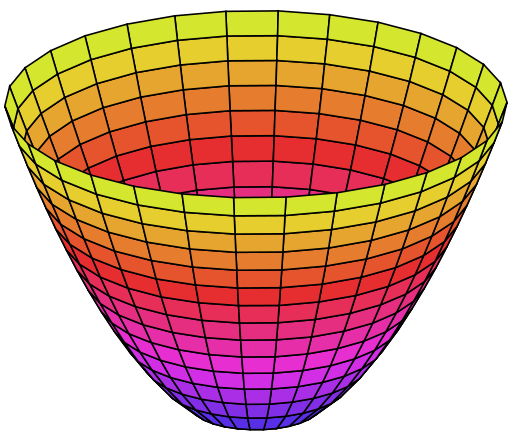
\includegraphics[scale=0.30]{imagenes/paraboloide.png}
\end{figure}

\subsection{El método}

Definimos

\[Q(x) = x^tAx - 2x^tb\]

Como $A$ es simétrica definida positiva, $Q$ resulta tener la forma deseada y además alcanza su mínimo absoluto en $x = A^{-1}b$. Para ver esto último notemos que podemos reescribir $Q(x) = (A^{-1}b - x)^t A (A^{-1}b - x) - b^{t}A^{-1}b$. Como $A$ es definida positiva entonces $(A^{-1}b - x)^t A (A^{-1}b - x) \geq 0$, con lo cual $Q(x) \geq -b^t A^{-1}b$. Luego $Q$ alcanzará el mínimo $-b^t A^{-1}b$ si y sólo si $(A^{-1}b - x)^t A (A^{-1}b - x) = 0 \Leftrightarrow A^{-1}b - x = 0$, nuevamente debido a que $A$ es definida positiva.

Fijemos un punto inicial $x^{(0)} \in \mathbb{R}^n$ y recorramos en dirección $d^{(0)} \in \mathbb{R}^n$ una cierta distancia dada por $\alpha_0 \in \mathbb{R}$, definiendo así un nuevo punto $x^{(1)} = x^{(0)} + \alpha_0 d^{(0)}$. Con este mismo razonamiento definimos una sucesión $\{x^{(k)}\}_k$ que es tal que

\[x^{(k + 1)} = x^{(k)} + \alpha_{k}d^{(k)}\]

Supongamos que la dirección $d^{(k)}$ está fija y es no nula, y miremos $Q(x^{(k + 1)}) = Q(x^{(k)} + \alpha d^{(k)})$ como función de $\alpha$. Si pensamos en la forma que tiene $Q(x)$ al mirarla sobre la recta $t(\alpha) = x^{(k)} + \alpha d^{(k)}$ obtendremos una parábola cóncava, y el punto de dicha parábola más cercano al mínimo será el punto crítico. Calculemos $D(Q(t(\alpha)))$,

\begin{align*}
D(Q(t(\alpha))) &= (\nabla Q(x^{(k)} + \alpha d^{(k)}))^t D(x^{(k)} + \alpha d^{(k)})\\
				&= (2A(x^{(k)} + \alpha d^{(k)}) - 2b)^t d^{(k)} \hspace{1.5cm}\text{(pues }\nabla Q(x) = 2Ax - 2b\text{)}\\
				&= 2(Ax^{(k)} - b + \alpha A d^{(k)})^t d^{(k)}\\
				&= 2(-(b - Ax^{(k)}) + \alpha A d^{(k)})^t d^{(k)}\\
				&= 2(-(b - Ax^{(k)})^t d^{(k)} + \alpha (d^{(k)})^t A^t d^{(k)})\\
				&= 2(-(b - Ax^{(k)})^t d^{(k)} + \alpha (d^{(k)})^t A d^{(k)})
\end{align*}

Llamemos $r^{(k)} = b - Ax^{(k)}$ al residuo (lo que falta para llegar a la solución). Entonces

\[D(Q(t(\alpha))) = 2(-(r^{(k)})^t d^{(k)} + \alpha (d^{(k)})^t A d^{(k)})\]


Como $d^{(k)} \neq 0$ y $A$ es definida positiva, entonces $(d^{(k)})^t A d^{(k)} \neq 0$. Luego, el mínimo se alcanza cuando

\[D(Q(t(\alpha))) = 0 \Leftrightarrow \alpha = \frac{(r^{(k)})^t d^{(k)}}{(d^{(k)})^t A d^{(k)}}\]

Entonces elegimos

\[\alpha_k = \frac{(r^{(k)})^t d^{(k)}}{(d^{(k)})^t A d^{(k)}}\]

De este modo, conociendo las direcciones, podemos calcular los $\alpha_k$ óptimos para cada paso.

\begin{obs}
Como $A$ es simétrica definida positiva, la forma $\Phi(x, y) = x^tAy$ es un producto interno. Notamos $\Phi(x, y) = \langle x, y \rangle_A$.
\end{obs}

\begin{obs}
Recordemos que dado un producto interno $\langle , \rangle$ y vectores $u, v \in \mathbb{R}^n$, la proyección ortogonal de $u$ sobre $v$ es

\[\text{proy}_{v}(u) = \frac{\langle u, v\rangle}{\langle v, v \rangle} v\]

Si escribimos a $u$ en una base de $\langle v \rangle \oplus \langle v \rangle^{\perp}$, entonces la proyección $\text{proy}_{v}(u)$ es la componente en la dirección de $v$. Geométricamente, esto es trazar un hiperplano perpendicular a $\langle v \rangle$ que pase por $u$ y tomar su intersección con $\langle v \rangle$. 
\end{obs}

Al producto interno canónico en $\mathbb{R}^n$, $\Phi(x, y) = x^ty$, lo notamos $\Phi(x, y) = \langle x, y \rangle_2$. Entonces podemos escribir

\[\alpha_k = \frac{\langle r^{(k)}, d^{(k)} \rangle_2}{\langle d^{(k)}, d^{(k)} \rangle_A} = 
\frac{\langle e^{(k)}, d^{(k)} \rangle_A}{\langle d^{(k)}, d^{(k)} \rangle_A}\]

donde $e^{(k)} = A^{-1}b - x^{(k)}$ es el error. Entonces $\alpha_k d^{(k)}$ es la proyección ortogonal de $e^{(k)}$ sobre $d^{(k)}$ para el producto interno $\langle , \rangle_A$. Esto muestra que en cada paso, el método suma la componente del error en la dirección dada.

\subsection{Elección de las direcciones}

Notemos que dependiendo de cómo elijamos las direcciones, convergeremos más o menos rápido, o inclusive podemos no converger. Por lo tanto, queremos estudiar cómo elegir las direcciones para converger al mínimo lo más rápido posible. Pensemos el problema para algunos casos particulares de $Q(x)$ en $\mathbb{R}^2$:

\begin{itemize}
\item $A$ diagonal y $b = 0$:

\[Q(x) = \begin{pmatrix}x_1 & x_2\end{pmatrix}
\begin{pmatrix}
a_{11} & 0\\
0 & a_{22}\\
\end{pmatrix}
\begin{pmatrix}
x_1 \\ x_2
\end{pmatrix} = a_{11}x_1^2 + a_{22}x_2^2
\]


Las curvas de nivel de $Q$ son elipses centradas en el origen. En este caso, conviene elegir una dirección paralela al eje $x$ y otra paralela al eje $y$.

\item $A$ diagonal y $b \neq 0$:

\[Q(x) = \begin{pmatrix}x_1 & x_2\end{pmatrix}
\begin{pmatrix}
a_{11} & 0\\
0 & a_{22}\\
\end{pmatrix}
\begin{pmatrix}
x_1 \\ x_2
\end{pmatrix} + \begin{pmatrix}x_1 & x_2\end{pmatrix}
\begin{pmatrix}
b_1 \\ b_2
\end{pmatrix}
 = a_{11}x_1^2 + a_{11}x_2^2 + b_1 x_1 + b_2 x_2
\]

Las curvas de nivel de $Q$ son elipses con centro $(x_0, y_0) \neq 0$. Conviene elegir una dirección paralela al eje $x = x_0$ y otra paralela al eje $y = y_0$.

\item En general:

Las curvas de nivel de $Q$ son elipses rotadas en un ángulo $\theta$, con centro $(x_0, y_0)$. Conviene elegir dos direcciones, cada una paralela a uno de los ejes rotados de las elipses.

\end{itemize}

Notemos que en todos los casos alcanzan con dos pasos para converger a la solución. Como es de esperarse, en $\mathbb{R}^n$ alcanzan $n$ pasos para asegurar la convergencia. Esto es lo que probaremos a continuación.

\begin{defi}
Sea $A \in \mathbb{R}^{n \times n}$ definida positiva. Dos vectores $x, y \in \mathbb{R}^n$ se dicen direcciones $A$-conjugadas si $x^t A y = 0$. En otras palabras, $x$ e $y$ son $A$-conjugadas si son vectores ortogonales para el producto interno $\langle,\rangle_A$.
\end{defi}

\begin{obs}
Si $x, y \in \mathbb{R}^n$ entonces $\langle x, y \rangle_A = x^t A y = (A^t x)^t y = \langle A^t x, y \rangle_2$. En particular, si $A$ es simétrica resulta que $\langle x, y \rangle_A = \langle Ax, y \rangle_2$, es decir que $x$ e $y$ son $A$-conjugadas si y sólo si $Ax$ e $y$ son ortogonales para el producto interno canónico.
\end{obs}

\begin{lema}
Sea $\{v_1, \cdots, v_n\} \subset \mathbb{R}^n$ un conjunto ortogonal para un producto interno $\langle, \rangle$ y de elementos no nulos. Entonces el conjunto es linealmente independiente.

\begin{proof}
Sea $\sum_{i = 1}^n \gamma_i v_i = 0$ una combinación lineal nula. Si $1 \leq k \leq n$ entonces

\[0 = \langle 0, v_k \rangle = \left\langle \sum_{i = 1}^n \gamma_i v_i, v_k \right\rangle = \sum_{i = 1}^n \gamma_i \langle v_i, v_k \rangle\]

Dado que el conjunto es ortogonal, todos los términos de la suma son cero salvo para $i = k$,

\[0 = \gamma_k \langle v_k, v_k \rangle = \gamma_k \norm{v_k}^2\]

Como $v_k \neq 0$, deducimos que $\gamma_k = 0$. Como $k$ es cualquiera, concluimos que el conjunto es l.i.
\end{proof}
\end{lema}

\begin{lema}
\label{lema:zero}
Sea $w \in \mathbb{R}^n$ y $\{v_1, \cdots, v_n\} \subset \mathbb{R}^n$ un conjunto ortogonal para un producto interno $\langle, \rangle$ y de elementos no nulos. Si $\langle w, v_i \rangle = 0$ para todo $i = 1, \cdots, n$, entonces $w = 0$.

\begin{proof}
Como $\{v_1, \cdots, v_n\}$ es ortogonal y no contiene al cero, entonces es l.i. Como tiene $n$ elementos, entonces es una base. Sea $w = \sum_{i = 1}^n \gamma_i v_i$ la escritura de $w$ en la base dada. Entonces

\[0 = \langle w, v_k \rangle = \left\langle \sum_{i = 1}^n \gamma_i v_i, v_k \right\rangle = \sum_{i = 1}^n \gamma_i \langle v_i, v_k \rangle = \gamma_k \norm{v_k}^2\]

En la última igualdad usamos la ortogonalidad de los elementos de la base. Como $v_k \neq 0$ entonces $\gamma_k = 0$, y como $k$ es cualquiera, resulta que $w = 0$.
\end{proof}
\end{lema}

El resultado fundamental es el siguiente,

\begin{propo}
Sea $A \in \mathbb{R}^{n \times n}$ s. d. p. Sean $d^{(0)}, \cdots, d^{(n - 1)}$ direcciones $A$-conjugadas de a pares y no nulas. Sea $\{x^{(k)}\}_k$ definida como antes. Entonces $Ax^{(n)} = b$, es decir que el método del gradiente conjugado converge a lo sumo en $n$ pasos.

\begin{proof}
Queremos ver que $x^{(n)} - A^{-1}b = 0$. Como las direcciones son ortogonales de a pares para el p. i. $\langle, \rangle_A$, entonces $\{d^{(0)}, \cdots, d^{(n - 1)}\}$ forman un conjunto ortogonal para ese p. i. Como ninguna es nula, por el Lema \ref{lema:zero} basta ver que $\langle x^{(n)} - A^{-1}b, d^{(k)}\rangle_A = 0$ para todo $k = 0, \cdots, n - 1$. Equivalentemente, $\langle Ax^{(n)} -b , d^{(k)}\rangle_2 = 0$ para todo $k$. 

Es fácil ver que si $k > 0$, $x^{(k)} = x^{(0)} + \sum_{i = 0}^{k - 1} \alpha_i d^{(i)}$. Luego

\begin{align*}
\langle Ax^{(n)} - b, d^{(k)} \rangle_2 & = \left\langle A \left(x^{(0)} + \sum_{i = 0}^{n - 1} \alpha_i d^{(i)}\right) - b, d^{(k)} \right\rangle_2 \\
& = \left\langle Ax^{(0)} + \sum_{i = 0}^{n - 1} \alpha_i A d^{(i)} - b, d^{(k)} \right\rangle_2\\
& = \langle Ax^{(0)} - b, d^{(k)} \rangle + \sum_{i = 0}^{n - 1} \alpha_i \langle Ad^{(i)}, d^{(k)}\rangle_2
\end{align*}

Como las direcciones son ortogonales resulta que $\langle Ad^{(i)}, d^{(k)} \rangle_2 = \langle d^{(i)}, d^{(k)} \rangle_A = 0$ si $i \neq k$. Obtenemos así,

\[\langle Ax^{(n)} - b, d^{(k)} \rangle_2 = \langle Ax^{(0)} - b, d^{(k)} \rangle_2 + \alpha_k \langle Ad^{(k)}, d^{(k)} \rangle_2 \]

Calculemos $\alpha_k \langle Ad^{(k)}, d^{(k)} \rangle_2$,

\begin{align*}
\alpha_k \langle Ad^{(k)}, d^{(k)} \rangle_2 &= \frac{\langle r^{(k)}, d^{(k)} \rangle_2}{\langle Ad^{(k)}, d^{(k)} \rangle_2} \langle Ad^{(k)}, d^{(k)} \rangle_2\\
& = \langle r^{(k)}, d^{(k)} \rangle_2\\
& = \langle b - Ax^{(k)}, d^{(k)} \rangle_2\\
& = \langle b, d^{(k)} \rangle_2 - \langle Ax^{(k)}, d^{(k)} \rangle_2
\end{align*}

Calculemos $\langle Ax^{(k)}, d^{(k)} \rangle_2$,

\begin{align*}
\langle Ax^{(k)}, d^{(k)} \rangle_2 &= \left\langle Ax^{(0)} + \sum_{i = 0}^{k - 1} \alpha_i A d^{(i)}, d^{(k)} \right\rangle_2 \\
& = \langle Ax^{(0)}, d^{(k)}\rangle_2 + \sum_{i = 0}^{k - 1} \alpha_i \langle A d^{(i)}, d^{(k)} \rangle_2\\
& = \langle Ax^{(0)}, d^{(k)}\rangle_2
\end{align*}

Entonces

\[\alpha_k \langle Ad^{(k)}, d^{(k)} \rangle_2 = \langle b, d^{(k)} \rangle_2 - \langle Ax^{(0)}, d^{(k)}\rangle_2 = \langle b - Ax^{(0)}, d^{(k)} \rangle_2\]

Finalmente

\[\langle Ax^{(n)} - b, d^{(k)} \rangle_2 = \langle Ax^{(0)} - b, d^{(k)} \rangle_2 + \langle b - Ax^{(0)}, d^{(k)} \rangle_2 = 0\]

que es lo que queríamos probar.

\end{proof}
\end{propo}

\subsection{Generación de direcciones $A$-conjugadas}

La forma de generar direcciones $A$-conjugadas se basa en el proceso de ortogonalización de Gram-Schmidt. Repasemos este último. Dada una base $\{v_1, \cdots, v_n\}$ de $\mathbb{R}^n$, el proceso genera una base ortogonal $\{w_1, \cdots, w_n\}$ para un producto interno $\langle, \rangle$. Más aún, estos vectores generados son de la forma

\[w_k = v_k - \sum_{i = 1}^{k - 1}\frac{\langle v_k, w_i\rangle}{\langle w_i, w_i \rangle} w_i\]

Generamos una secuencia de direcciones $A$-conjugadas del siguiente modo. Fijado $x^{(0)}$, definimos $d^{(0)} = -r^{(0)}$. Para $k > 0$ definimos

\[d^{(k)} = -r^{(k)} - \frac{\langle-r^{(k)}, d^{(k - 1)}\rangle_A}{\langle d^{(k - 1)}, d^{(k - 1)} \rangle_A} d^{(k - 1)}\]

Los vectores $-r^{(k)}$ juegan el papel de los $v_k$, y los $d^{(k)}$ el de los $w_k$. La razón de que $d^{(k)}$ sólo dependa de $d^{(k - 1)}$ y no de $d^{(j)}$ con $j < k - 1$ (como en el esquema anterior de Gram-Schmidt) es que $\langle -r^{(k)} , d^{(j)} \rangle_A = 0$ para $j < k - 1$. Entonces los vectores $d^{(0)}, \cdots, d^{(n - 1)}$ así generados son ortogonales respecto del producto interno $\langle , \rangle_A$, es decir, son $A$-conjugados.

\subsection{Comparación con Cholesky}

Hemos visto que en el caso de $A$ simétrica definida positiva, la resolución de $Ax = b$ se puede hacer vía la factorización de Cholesky. El método del gradiente conjugado es iterativo, con lo cual las ventajas frente al método directo son las anteriormente mencionadas.
\newpage
\section{Descomposición en valores singulares}

\subsection{Problema}

Dada $A \in \mathbb{R}^{m \times n}$ queremos descomponer $A = U \Sigma V^t$ con $U \in \mathbb{R}^{m \times m}$ ortogonal, $\Sigma \in \mathbb{R}^{m \times n}$ diagonal y $V\in \mathbb{R}^{n \times n}$ ortogonal.

\subsection{Lemas auxiliares}

Para llegar al resultado principal de esta sección necesitaremos algunos resultados auxiliares.

\begin{obs}
El producto interno canónico en $\mathbb{C}^n$ es la forma $\Phi: \mathbb{C}^n \times \mathbb{C}^n \to \mathbb{C}$ tal que

\[\Phi(x, y) = x^t \overline{y}\]

donde $\overline{y}$ es la conjugación de $y$ coordenada a coordenada. Notar que restringido a $\mathbb{R}^n$, coincide con el producto interno canónico en $\mathbb{R}^n$.
\end{obs}

En lo que sigue, todos los productos internos considerados serán el canónico en $\mathbb{C}^n$, y lo notaremos con $\langle, \rangle$.

\begin{obs}
Si $\alpha \in \mathbb{C}$ y $x, y \in \mathbb{C}^n$, entonces

\[\langle \alpha x, y \rangle = (\alpha x)^t \overline{y} = \alpha x^t \overline{y} = \alpha \langle x, y \rangle\]

\[\langle x, \alpha y \rangle = x^t \overline{\alpha y} = x^t (\overline{\alpha} \hspace{1mm} \overline{y}) = \overline{\alpha} x^t \overline{y} = \overline{\alpha} \langle x, y \rangle\]
\end{obs}

\begin{obs}
Si $A \in \mathbb{R}^{n \times n}$ es simétrica y $v, w \in \mathbb{C}^n$, entonces

\[\langle Av, w \rangle = (Av)^t \overline{w} = v^t A^t \overline{w} = v^t A \overline{w} = v^t \overline{\overline{A} w} = v^t \overline{A w} = \langle v, Aw \rangle\]
\end{obs}

\begin{lema}
\label{lema:autovreales}
Sea $A \in \mathbb{R}^{n \times n}$ simétrica. Entonces todos sus autovalores son reales.

\begin{proof}
Sea $\lambda \in \mathbb{C}$ un autovalor de $A$. Sea $v \in \mathbb{C}^n$ un autovector asociado. Entonces

\[\langle Av, v \rangle = \langle \lambda v, v \rangle = \lambda \langle v, v \rangle = \lambda \norm{v}^2\]

Por otro lado,

\[\langle Av, v \rangle = \langle v, Av \rangle = \langle v, \lambda v \rangle = \overline{\lambda}\langle v, v \rangle = \overline{\lambda} \norm{v}^2\]

Luego $\lambda \norm{v}^2 = \langle Av, v \rangle = \overline{\lambda} \norm{v}^2$, es decir que $\lambda \norm{v}^2 = \overline{\lambda} \norm{v}^2$. Como $v \neq 0$ por ser autovector, entonces $\lambda = \overline{\lambda}$, por lo que concluimos que $\lambda \in \mathbb{R}$.
\end{proof}
\end{lema}

\begin{lema}
Sea $A \in \mathbb{R}^{n \times n}$ simétrica. Si $\lambda \in \mathbb{R}$ es autovalor de $A$ entonces $\lambda$ tiene un autovector asociado con coordenadas reales.

\begin{proof}
Sea $v \in \mathbb{C}^n$ un autovector asociado a $\lambda$. Si todas las coordenadas de $v$ son imaginarios puros, entonces definimos $w = iv$, que tiene todas las coordenadas reales. Además $w \neq 0$ porque $v \neq 0$. Se tiene

\[Aw = A(iv) = iAv = i(\lambda v) = \lambda (iv) = \lambda w\]

Entonces $w \in \mathbb{R}^n$ es un autovector asociado a $\lambda$.

Veamos el caso en que $v$ tiene alguna coordenada que no es imaginario puro. Consideramos $w = v + \overline{v}$. Es claro que $w$ es un vector de números reales. La coordenada que en $v$ no era un imaginario pura tiene parte real no nula, con lo cual esa misma coordenada es no nula en $w$. Luego $w \neq 0$. Además, usando que $A$ y $\lambda$ son reales,

\[Aw = A(v + \overline{v}) = Av + A\overline{v} = Av + \overline{\overline{A}v} = Av + \overline{Av} = \lambda v + \overline{\lambda v} = \lambda v + \overline{\lambda} \overline{v} = \lambda v + \lambda \overline{v} = \lambda(v + \overline{v}) = \lambda w \]

Luego $w \in \mathbb{R}^n$ es un autovector asociado a $\lambda$.
\end{proof}
\end{lema}

\begin{propo}
Sea $A \in \mathbb{R}^{n \times n}$ simétrica. Entonces existen $Q \in \mathbb{R}^{n \times n}$ ortogonal y $D \in \mathbb{R}^{n \times n}$ diagonal tal que

\[A = Q D Q^t\]
\begin{proof}

Inducción en $n \in \mathbb{N}$.

Si $n = 1$, $A = \begin{pmatrix} a \end{pmatrix}$ para cierto $a \in \mathbb{R}$, y tomamos $Q = \begin{pmatrix} 1 \end{pmatrix}$ y $D = \begin{pmatrix} a \end{pmatrix}$.

Sea $n > 1$. Sea $\lambda \in \mathbb{R}$ un autovalor de $A$, y $v \in \mathbb{R}^n$ un autovector asociado con coordenadas reales,  normalizado. Completamos $v$ a una base de $\mathbb{R}^n$, con $v_2, \cdots, v_n$. A la base $\{v, v_2, \cdots, v_n\} \subset \mathbb{R}^n$ le aplicamos el proceso de ortogonalización de Gram-Schmidt, obteniendose $\{v, w_2, \cdots, w_n\} \subset \mathbb{R}^n$. Sea 

\[W = \left(\begin{array}{c|c|c}
& &\\
w_2 & \cdots & w_n\\
& &
\end{array}\right) \in \mathbb{R}^{n \times (n - 1)}\]

A partir de esta, definimos

\[U = \left(\begin{array}{c|ccc}
& & &\\
v& & W &\\
& & &
\end{array}\right) \in \mathbb{R}^{n \times n}\]

Entonces 

\begin{align*}
U^t A U &= \left(\begin{array}{ccc}
& v^t& \\\hline
& & \\
& W^t & \\
& &
\end{array}\right) A \left(\begin{array}{c|ccc}
& & &\\
v& & W &\\
& & &
\end{array}\right)\\
&= \left(\begin{array}{ccc}
& v^t A& \\\hline
& & \\
& W^t A & \\
& &
\end{array}\right)\left(\begin{array}{c|ccc}
& & &\\
v& & W &\\
& & &
\end{array}\right)\\
&= \left(\begin{array}{c|c}
v^t A v & v^t A W\\\hline
W^t A u & W^t A W
\end{array}\right)
\end{align*}

Tenemos que

\[v^t A v = v^t (\lambda v) = \lambda v^t v = \lambda \norm{v}^2 = \lambda\]

Además $W^tAv = W^t (\lambda v) = \lambda W^t v$, y como las filas de $W^t$ son ortogonales a $v$ entonces

\[W^t Av = 0\]

Análogamente

\[v^tAW = (A^tv)^tW = (Av)^tW = (\lambda v)^t W = \lambda v^t W = 0\]

Luego

\[U^t A U = \left(\begin{array}{c|ccc}
1 & 0 & \cdots & 0\\ \hline
0 & & & \\
\vdots & & W^tAW &\\
0 & & &
\end{array}\right)\]

Resta calcular el bloque $W^tAW$. Como $W^tAW \in \mathbb{R}^{(n - 1) \times (n - 1)}$ es simétrica, entonces por hipótesis inductiva existen $\tilde{P} \in \mathbb{R}^{(n - 1) \times (n - 1)}$ ortogonal y $\tilde{D} \in \mathbb{R}^{(n - 1) \times (n - 1)}$ diagonal, tal que $W^t A W = \tilde{P}\tilde{D}\tilde{P}^t$. Extendemos $\tilde{P}$ definiendo

\[P = \left(\begin{array}{c|ccc}
1 & 0 & \cdots & 0\\ \hline
0 & & & \\
\vdots & & \tilde{P} &\\
0 & & &
\end{array}\right) \in \mathbb{R}^{n \times n}\]

A $\tilde{D}$ la extendemos del siguiente modo

\[D = \left(\begin{array}{c|ccc}
\lambda & 0 & \cdots & 0\\ \hline
0 & & & \\
\vdots & & \tilde{D} &\\
0 & & &
\end{array}\right) \in \mathbb{R}^{n \times n}\]

Notemos que, como $\tilde{P}$ es ortogonal, entonces $P$ también lo es. Análogamente, como $\tilde{D}$ es triangular superior, entonces $D$ también lo es. Luego

\begin{align*}
PDP^t &= \left(\begin{array}{c|ccc}
1 & 0 & \cdots & 0\\ \hline
0 & & & \\
\vdots & & \tilde{P} &\\
0 & & &
\end{array}\right)
\left(\begin{array}{c|ccc}
\lambda & 0 & \cdots & 0 \\ \hline
0 & & & \\
\vdots & & \tilde{D} &\\
0 & & &
\end{array}\right)
\left(\begin{array}{c|ccc}
1 & 0 & \cdots & 0\\ \hline
0 & & & \\
\vdots & & \tilde{P}^t &\\
0 & & &
\end{array}\right)\\
&= \left(\begin{array}{c|ccc}
\lambda & 0 & \cdots & 0\\ \hline
0 & & & \\
\vdots & & \tilde{P}\tilde{D} &\\
0 & & &
\end{array}\right)
\left(\begin{array}{c|ccc}
1 & 0 & \cdots & 0\\ \hline
0 & & & \\
\vdots & & \tilde{P}^t &\\
0 & & &
\end{array}\right)\\
& = \left(\begin{array}{c|ccc}
\lambda & 0 & \cdots & 0\\ \hline
0 & & & \\
\vdots & & \tilde{P}\tilde{D}\tilde{P}^t &\\
0 & & &
\end{array}\right)\\
& = \left(\begin{array}{c|ccc}
\lambda & 0 & \cdots & 0\\ \hline
0 & & & \\
\vdots & & W^tAW &\\
0 & & &
\end{array}\right)\\
& = U^tAU
\end{align*}

Entonces $PDP^t = U^tAU$, con lo cual $A = (UP)D(UP)^t$. Poniendo $Q = UP \in \mathbb{R}^{n \times n}$ resulta que $Q$ es ortogonal por ser producto de matrices ortogonales, y $A = QDQ^t$, que es lo que queríamos demostrar.
\end{proof}
\end{propo}

\begin{lema}
En las condiciones de la proposición anterior, las columnas de $Q$ son autovectores de $A$ y los elementos de la diagonal de $D$ son autovalores de $A$. Más precisamente $col_i(Q)$ es autovector de $A$ de autovalor $D_{ii}$.

\begin{proof}
Se tiene

\[Q^tAQ = D \Rightarrow QQ^t AQ = QD \Rightarrow AQ = QD \Rightarrow col_i(AQ) = col_i(QD) \Rightarrow A\text{ }col_i(Q) = D_{ii}\text{ }col_i(Q)\]

Como $Q$ es ortogonal, en particular es inversible y por lo tanto no tiene columnas nulas. Luego, $col_i(Q) \neq 0$ es autovector de $A$ de autovalor $D_{ii}$.
\end{proof}
\end{lema}

\begin{teo}
\label{teo:diagonalizacion}
Sea $A \in \mathbb{R}^{n \times n}$ simétrica. Entonces existe una base ortonormal de $\mathbb{R}^n$ formada por autovectores reales de $A$.

\begin{proof}
Escribamos $A = QDQ^t$ como antes. Por el lema previo, las columnas de $Q$ son autovectores de $A$. Como $Q$ es es inversible, sus columnas son linealmente independientes y, por lo tanto, como son $n$, forman una base de $\mathbb{R}^n$. Más aún, son vectores ortogonales, pues $Q$ es ortogonal. Para que la base sea ortonormal, basta dividir cada vector por su norma.
\end{proof}
\end{teo}

\subsection{Teorema de descomposición en valores singulares}

\begin{teo}
Sea $A \in \mathbb{R}^{m \times n}$ arbitraria. Entonces existen $U \in \mathbb{R}^{m \times m}$ ortogonal, $V \in \mathbb{R}^{n \times n}$ ortogonal y $\Sigma \in \mathbb{R}^{m \times n}$ diagonal tal que

\[A = U \Sigma V^t\]

\begin{proof}
Vamos a descomponer la prueba en varios pasos.

\begin{enumerate}
\item \textbf{La matriz $AA^t \in \mathbb{R}^{m \times m}$ es simétrica.} Por la Proposición \ref{teo:diagonalizacion} existe una base ortonormal $\{u_1, \cdots, u_m\}$ de $\mathbb{R}^m$ formada por autovectores de $AA^t$. Sean $\lambda_1, \cdots, \lambda_m \in \mathbb{R}$ los autovalores asociados, todos reales por el Lema \ref{lema:autovreales}.

\item \textbf{Los autovalores $\lambda_1, \cdots, \lambda_m$ son no negativos.}

\begin{align*}
AA^tu_i = \lambda_i u_i 	&\Rightarrow u_i^t AA^t u_i = \lambda_i u_i^t u_i\\
						&\Rightarrow (A^tu_i)^t(A^tu_i) = \lambda_i \norm{u_i}_2^2\\
						&\Rightarrow \norm{A^tu_i}_2^2 = \lambda_i \norm{u_i}_2^2\\
						&\Rightarrow \lambda_i \geq 0 
\end{align*}

\item Supongamos sin pérdida de generalidad que $\lambda_1, \cdots, \lambda_r$ son los autovalores de $AA^t$ no nulos y definamos para cada $1 \leq i \leq r$,

\[\sigma_i = \sqrt{\lambda_i}\]
\[v_i = \frac{1}{\sigma_i} A^t u_i\]

Notemos que $v_i \neq 0$ porque $Av_i = \frac{1}{\sigma_i} AA^t u_i = \frac{\lambda_i}{\sigma_i} u_i \neq 0$. 

\item \textbf{Para cada $1 \leq i \leq r$, $v_i$ es autovector de $A^tA$ de autovalor $\lambda_i$.} Ya vimos que $v_i \neq 0$. Además

\[A^tAv_i = \frac{1}{\sigma_i}A^tAA^tu_i = \frac{\lambda_i}{\sigma_i}A^tu_i = \lambda_i v_i\]

\item \textbf{El conjunto $\{v_1, \cdots, v_r\}$ es ortonormal.}

\begin{align*}
v_i^t v_j = \left(\frac{A^t u_i}{\sigma_i}\right)^t \left(\frac{A^t u_j}{\sigma_j}\right)
&= \frac{1}{\sigma_i \sigma_j}u_i^t AA^t u_j\\
&= \frac{1}{\sigma_i \sigma_j} u_i^t \lambda_j u_j\\
&= \frac{\lambda_j}{\sigma_i \sigma_j} u_i^t u_j\\
&= \frac{\lambda_j}{\sigma_i \sigma_j} \delta_{ij}\\
&= \frac{\lambda_j}{\sqrt{\lambda_i} \sqrt{\lambda_j}} \delta_{ij}\\
&= \delta_{ij}
\end{align*}

\item Extendemos $\{v_1, \cdots, v_r\}$ a una base ortonormal de $\mathbb{R}^n$ con $v_{r + 1}, \cdots, v_n$. Definimos

\[U = \begin{pmatrix}
 & & \\
u_1 & \cdots & u_m\\
 & &
\end{pmatrix}
\hspace{1cm}
V = \begin{pmatrix}
 & & \\
v_1 & \cdots & v_n\\
 & &
\end{pmatrix}
\hspace{1cm}
\Sigma = \begin{pmatrix}
\sigma_1		&			&			&		& 			&		\\
			& \ddots		&			&		&	0		&		\\
			&			& \sigma_r 	&		&			&		\\
			&			&			& 0		&			&		\\
			&	0		&			&		& \ddots		&		\\
			&			&			&		&			& 0
\end{pmatrix}\]

\item Veamos que $A = U \Sigma V^t$. Como $U$ y $V$ son ortogonales, es lo mismo ver que $U^t A V = \Sigma$. Se tiene

\begin{align*}
(U^tAV)_{ij} & = fil_i(U^tA) \text{ }col_j(V)\\
			& = fil_i(U^t)A \text{ }col_j(V)\\
			& = col_i(U)^tA \text{ }col_j(V)\\
			& = u_i^t A v_j
\end{align*}

Separemos en casos:

\begin{itemize}
\item Si $j \leq r$:

En este caso $v_j = \frac{1}{\sigma_j}A^t u_j$, con lo cual

\begin{align*}
u_i^t A v_j &= \frac{1}{\sigma_j} u_i^t AA^t u_j				&\\
			&= \frac{1}{\sigma_j} u_i^t (\lambda_j u_j)		&\\
			&= \frac{\lambda_j}{\sigma_j}u_i^t u_j			&\\
			&= \frac{\sigma_j^2}{\sigma_j} \delta_{ij}		&& \text{(pues } \{u_1, \cdots, u_m\} \text{ es ortonormal)} \\\\
			&= \sigma_j \delta_{ij}							&
\end{align*}

\item Si $j > r$:

\begin{itemize}
\item Si $i \leq r$:

En este caso $v_i = \frac{1}{\sigma_i} A^t u_i \Rightarrow \sigma_i v_i = A^t u_i$, con lo cual

\begin{align*}
u_i^t A v_j &= (u_i^t A v_j)^t			& \\
			&= v_j^t A^t u_i				& \\
			&= v_j^t (\sigma_i v_i)		& \\
			&= \sigma_i v_j^t v_i		& \\
			&= \sigma_i \delta_{ij}		& \text{(pues } \{v_1, \cdots, v_n\} \text{ es ortonormal)} \\
			&= 0							& \text{(pues }i \leq r < j \text{)} \\
\end{align*}

\item Si $i > r$:

Tenemos entonces que $\lambda_i = 0$. Veamos que necesariamente $A^t u_i = 0$. Por el absurdo supongamos que $A^t u_i \neq 0$, entonces $0 \neq \norm{A^t u_i}_2^2 = (A^t u_i)^t(A^t u_i) = u_i^t A A^t u_i = u_i^t (\lambda_i u_i) = \lambda_i u_i^t u_i = \lambda_i \norm{u_i}_2^2$. Luego $0 \neq \lambda_i \norm{u_i}_2^2 \Rightarrow \lambda_i \neq 0$, absurdo.

Como $A^t u_i = 0$ entonces

\[u_i^t A v_j = (u_i^t A v_j)^t = v_j^t A^t u_i = 0\]
\end{itemize}
\end{itemize}
\end{enumerate}
\end{proof}
\end{teo}

Los elementos no nulos de la diagonal de $\Sigma$, $\sigma_1, \cdots, \sigma_r$, se llaman valores singulares de $A$. Si bien la descomposición en valores singulares no es única, las matrices $U$, $\Sigma$ y $V$ siempre cumplen ciertas propiedades

\begin{propo}
Sea $A = U \Sigma V^t$ una descomposición en valores singulares. Sean $\sigma_1, \cdots, \sigma_r$ los valores singulares. Sean $u_1, \cdots, u_m$ las columnas de $U$, y $v_1, \cdots, v_n$ las columnas de $V$. Entonces
\begin{itemize}
\item $u_i$ es autovector de $AA^t$.
\item $v_i$ es autovector de $A^tA$.
\end{itemize}
En ambos casos, si $i \leq r$ entonces el autovalor asociado es $\sigma_i^2$ y es 0 en caso contrario.

\begin{proof}
Tenemos que

\[AA^t = (U \Sigma V^t)(U \Sigma V^t)^t = U \Sigma V^t V \Sigma^t U^t = U \Sigma \Sigma^t U^t\]

Notemos que $\Sigma \Sigma^t = \overline{\Sigma} = \text{diag}(\sigma_1^2, \cdots, \sigma_r^2, 0, \cdots, 0) \in \mathbb{R}^{m \times m}$. Entonces

\[AA^tu_i = U \overline{\Sigma} U^t u_i = U \overline{\Sigma} e_i = U \text{ } col_i(\overline{\Sigma})\]

Si $i \leq r$ entonces $col_i(\overline{\Sigma}) = \sigma_i^2 e_i$ con lo cual $AA^t u_i = \sigma_i^2 U e_i = \sigma_i^2 u_i$, es decir que $u_i$ es autovector de $AA^t$ de autovalor $\sigma_i^2$. Si $i > r$ entonces $col_i(\overline{\Sigma}) = 0$ con lo cual $u_i$ es autovector de autovalor 0.

Para los $v_i$ la demostración es igual.
\end{proof}
\end{propo}
\newpage
\section{Cuadrados mínimos lineales}

\subsection{Problema}

Supongamos que disponemos de una muestra de valores provenientes de un experimento

\begin{center}
\begin{tabular}{c|c}
$x$ & $y$\\
\hline
$x_1$ & $y_1$\\
$x_2$ & $y_2$\\
$\vdots$ & $\vdots$\\
$x_m$ & $y_m$
\end{tabular}
\end{center}

y queremos encontrar una relación entre los valores de $x$ e $y$. Tenemos dos opciones:

\begin{enumerate}
\item Encontrar una función $f$ tal que $f(x_i) = y_i$ para todo $i = 1, \cdots, m$.
\item Encontrar una función $f$ tal que $f(x_i) \approx y_i$ para todo $i = 1, \cdots, m$.
\end{enumerate}

Cuando tratamos con muestras observadas, en general estamos lidiando con valores que ya poseen un error, proveniente de la medición. Esto implica que buscar relaciones exactas (del tipo 1) pierda sentido pues en realidad sólo conocemos aproximaciones de los valores reales. Por este motivo, nos concentraremos en la opción 2.

Suponiendo que contamos con una familia de funciones $\mathcal{F}$ de la cual queremos extraer una de ellas, necesitamos un criterio para comparar funciones que contiene. Tres criterios posibles son:

\begin{itemize}
\item $\min\limits_{f \in \mathcal{F}}\max\limits_{1 \leq i \leq m} |f(x_i) - y_i|$

Minimiza el máximo error en un punto. La desventaja de este criterio es que es muy susceptible a la presencia de outliers (valores atípicos).

\item $\min\limits_{f \in \mathcal{F}} \sum_{i = 1}^m |f(x_i) - y_i|$

Minimiza el error. Este criterio sobrepasa el problema de los outliers. La desventaja que tiene es que queremos encontrar el mínimo de una función que involucra un valor absoluto, que sabemos que no es derivable en el origen, lo cual dificulta la tarea.

\item $\min\limits_{f \in \mathcal{F}} \sum_{i = 1}^m (f(x_i) - y_i)^2$

Minimiza el error cuadrático. Este criterio no padece de ninguno de los problemas anteriores.
\end{itemize}

Utilizaremos este último criterio. La familia de funciones que vamos a considerar es

\[\mathcal{F} = \{a_1 \phi_1 + \cdots + a_n \phi_n : a_1, \cdots, a_n \in \mathbb{R}\}\]

donde las funciones reales $\phi_1, \cdots, \phi_n$ están fijas. En otras palabras, estamos considerando el subespacio de funciones

\[\mathcal{F} = \langle\phi_1, \cdots, \phi_n\rangle_{\mathbb{R}}\]

Entonces el problema es encontrar los coeficientes $a_1, \cdots, a_n$ que realizan el mínimo

\[\min\limits_{a_1, \cdots, a_n \in \mathbb{R}} \sum_{i = 1}^m (a_1 \phi_1(x_i) + \cdots + a_n \phi_n(x_i) - y_i)^2\]

Consideremos

\[A = \begin{pmatrix}
\phi_1(x_1) & \cdots & \phi_n(x_1) \\
\phi_1(x_2) & \cdots & \phi_n(x_2) \\
\vdots		&		&	\vdots		\\
\phi_1(x_n)	& \cdots & \phi_n(x_n)
\end{pmatrix} 
\hspace{1cm}
x = \begin{pmatrix}
a_1 \\
\vdots \\
a_n
\end{pmatrix}
\hspace{1cm}
b = \begin{pmatrix}
y_1\\
\vdots\\
y_m
\end{pmatrix}
\]

Entonces el mínimo a calcular lo podemos escribir como

\[\min \limits_{x \in \mathbb{R}^n} \norm{Ax - b}_2^2\]

\begin{obs}
\hspace{1cm}
\begin{enumerate}
\item No necesitamos conocer el valor de las $\phi_i$ en todo su dominio, sino sólo en los puntos $x_1, \cdots, x_m$.
\item Para que el problema tenga sentido necesitamos más datos que incógnitas, i.e., $m \geq n$.
\end{enumerate}
\end{obs}

Abstrayéndonos de las funciones $\phi_1, \cdots, \phi_n$ y de las muestras $(x_1, y_1), \cdots, (x_m, y_m)$, definimos el problema de cuadrados mínimos lineales del siguiente modo. Dadas $A \in \mathbb{R}^{m \times n}$ y $b \in \mathbb{R}^m$, hallar $x \in \mathbb{R}^{n}$ que minimice $\norm{Ax - b}_2^2$.

Lo estudiaremos y atacaremos desde un punto de vista puramente algebraico.

\subsection{Intuición geométrica}

En primer lugar, observemos que si el sistema $Ax = b$ tiene solución, entonces cualquiera de ellas realiza el mínimo, que es 0.

Si $Ax = b$ no tiene solución, entonces es evidente que el mínimo es mayor que 0. Para entender cómo elegir un vector $x$ que lo realice, pensemos en $Ax$ y $b$ como vectores en $\mathbb{R}^m$. El mínimo se alcanza cuando la distancia euclídea entre estos dos vectores es mínima. Pero el único de estos dos vectores que se mueve es $Ax$, con lo cual hay que elegirlo de modo tal que esté lo más cerca posible de $b$. Recordemos que el conjunto de valores que puede tomar $Ax$ es el subespacio $\text{Im}(A) = \{Ax : x\in \mathbb{R}^n\}$. Luego, queremos encontrar la distancia del punto $b$ al subespacio $\text{Im}(A)$, y es sabido que el punto sobre el subespacio que realiza la distancia es la proyección ortogonal de $b$ sobre $\text{Im}(A)$.

\begin{figure}[h]
\centering
\input{imagenes/proyeccion.pdf_tex}
\end{figure}

En la figura, $b_1 = \text{proy}_{\text{Im}(A)}(b)$ es el punto que realiza la distancia, $b_2 = \text{proy}_{\text{Im}(A)^{\perp}}(b)$, y $x_1$ y $x_2$ son soluciones.

\subsection{Solución}

Como $\mathbb{R}^m = \text{Im}(A) \oplus \text{Im}(A)^{\perp}$ entonces $b$ se escribe en forma única como $b = b_1 + b_2$ con $b_1 \in \text{Im}(A)$ y $b_2 \in \text{Im}(A)^{\perp}$. Recordemos que $b_1$ es la proyección ortogonal de $b$ sobre $\text{Im}(A)$ y $b_2$ es la proyección ortogonal de $b$ sobre $\text{Im}(A)^{\perp}$.

\begin{propo}
Sea $b = b_1 + b_2$ la escritura en forma única como $b_1 \in \text{Im}(A)$ y $b_2 \in \text{Im}(A)^{\perp}$. Entonces el mínimo $\min\limits_{x \in  \mathbb{R}^n}\norm{Ax - b}_2^2$ se realiza únicamente cuando $Ax = b_1$.

\begin{proof}
\begin{align*}
\norm{Ax - b}_2^2 &= \norm{Ax - (b_1 + b_2)}_2^2				&\\
				&= \norm{(Ax - b_1) + b_2}_2^2				&\\
				&= \norm{Ax - b_1}_2^2 + \norm{b_2}_2^2		&\text{(por Pitágoras)}\\
				&\geq \norm{b_2}_2^2
\end{align*}

Entonces el mínimo se realiza sí y sólo si $\norm{Ax - b_1}_2^2 = 0 \Leftrightarrow Ax = b_1$.

\end{proof}
\end{propo}

Observemos que como $b_1 \in \text{Im}(A)$ entonces siempre existe un vector $x$ que realiza el mínimo. Es decir, cuadrados mínimos lineales siempre tiene solución. Estudiemos ahora la unicidad de la misma.

Es importante notar que la unicidad no depende del conjunto $\text{Im}(A)$ si no de cómo la matriz $A$ transforma los vectores. En términos de los elementos de la matriz, tenemos el siguiente resultado,

\begin{propo}
La solución de cuadrados mínimos lineales es única si y sólo el rango columna de $A$ es completo, es decir, sus columnas son LI. Notar que en caso de ser cuadrada esto implica que $A$ tiene que ser inversible, pero en ese caso $b \in Im(A)$ y podemos usar otro método para resolver el sistema.

\begin{proof}
Existirá un único $x \in \mathbb{R}^n$ tal que $Ax = b_1$ si y sólo si la matriz $A$ es inversible.
\end{proof}
\end{propo}

\subsection{Ecuaciones normales}

Nuestro próximo objetivo es caracterizar la solución en términos de $A$ y de $b$.

\begin{lema}
$\text{Im}(A)^{\perp} = \text{Nu}(A^t)$.

\begin{proof}
($\subseteq$) Sea $v \in \text{Im}(A)^{\perp}$, entonces $\langle w, v \rangle_2 = 0$ para todo $w \in \text{Im}(A)$. Queremos ver que $v \in \text{Nu}(A^t)$.

Se tiene

\[A^tv = \begin{pmatrix}
fil_1(A^t)v\\
\vdots\\
fil_n(A^t) v
\end{pmatrix} = \begin{pmatrix}
col_1(A)^t v\\
\vdots\\
col_n(A)^t v
\end{pmatrix} = \begin{pmatrix}
\langle col_1(A), v \rangle_2\\
\vdots\\
\langle col_n(A), v \rangle_2
\end{pmatrix} = 0\]

pues $col_i(A) \in \text{Im}(A)$ para todo $i$.\\[0.25cm]

($\supseteq$) Sea $v \in \text{Nu}(A^t)$, entonces $A^tv = 0$. Sea $w \in \text{Im}(A)$, queremos ver que $\langle w, v \rangle_2 = 0$.

Como $w \in \text{Im}(A)$, entonces $Az = w$ para algún $z \in \mathbb{R}^n$. Luego $w^t = z^tA^t$ con lo cual $\langle w, v \rangle_2 = w^tv = z^tA^tv = 0$. 
\end{proof}
\end{lema}

\begin{propo}
$x \in \mathbb{R}^{n}$ es solución de cuadrados mínimos lineales si y sólo si $A^tAx = A^tb$.

\begin{proof}
($\Rightarrow$) Sea $x$ una solución. Escribamos $b = b_1 + b_2$ con $b_1 \in \text{Im}(A)$ y $b_2 \in \text{Im}(A)^{\perp}$. Entonces $Ax = b_1 \Rightarrow A^tAx = A^tb_1$. Como $\text{Im}(A)^{\perp} = \text{Nu}(A^t)$ entonces $A^tb_2 = 0$, con lo cual $A^tAx = A^tb_1 = A^tb_1 + A^tb_2 = A^t(b_1 + b_2) = A^tb$.\\[0.25cm]

($\Leftarrow$) Sea $x$ tal que $A^tAx = A^tb = A^t(b_1 + b_2) = A^tb_1 \Rightarrow A^tAx - A^tb_1 = 0 \Rightarrow A^t(Ax - b_1) = 0 \Rightarrow Ax - b_1 \in \text{Nu}(A^t) = \text{Im}(A)^{\perp}$. Entonces $Ax - b_1 \in \text{Nu}(A^t) = \text{Im}(A)^{\perp} \cap \text{Im}(A) = \{0\} \Rightarrow Ax = b_1$ entonces $x$ es solución de cuadrados mínimos lineales.
\end{proof}
\end{propo}

Entonces resolver cuadrados mínimos equivale a resolver el sistema $A^tAx = A^tb$. Este sistema de ecuaciones recibe el nombre de \textit{ecuaciones normales}. Sin embargo, la resolución vía este sistema puede no ser númericamente estable, pues la matriz $A^tA$ suele estar mal condicionada aún estando $A$ bien condicionada. Por ejemplo,

\[A = \begin{pmatrix}
1 & 1\\
\varepsilon & 0 \\
0 & \varepsilon
\end{pmatrix}
\hspace{1cm}
A^tA = \begin{pmatrix}
1 + \varepsilon^2 & 1\\
1 & 1 + \varepsilon^2
\end{pmatrix}\]

En este caso $A^tA$ está muy mal condicionada. Si $\varepsilon$ es chico, entonces $\varepsilon^2$ es despreciable, y en un contexto de aritmética finita puede ser absorbido en la suma, obteniéndose $fl(fl(1) + fl(\varepsilon^2)) = 1$. Con este redondeo resulta que $A^tA = \begin{pmatrix}1 & 1 \\ 1 & 1 \end{pmatrix}$ de modo que las ecuaciones normales tendrán infinitas soluciones. Sin embargo $A$ tiene columnas l. i. con lo cual la solución de cuadrados mínimos es única.

\subsection{Resolución por QR}

Sean $A \in \mathbb{R}^{m \times n}$ y $b \in \mathbb{R}^m$ y supongamos sin pérdida de generalidad que $m \geq n$ (si no fuera este el caso, agregamos filas de 0 en $A$ y $b$). Sea $A = QR$ su factorización QR. Como $Q^t$ preserva norma 2 entonces

\[\norm{Ax - b}_2^2 = \norm{Q^t(Ax - b)}_2^2 = \norm{Q^t(QRx - b)}_2^2 = \norm{Rx - Q^tb}_2^2\]

Tenemos dos casos:
\begin{itemize}
\item Las columnas de $A$ son l. i.:

Como $Q$ es inversible entonces $\text{rg}(A) = \text{rg}(R)$. Entonces, en este caso, las columnas de $R$ también son l. i. y por lo tanto tiene la forma

\[R = \begin{pmatrix}
& 		& \\
& R_1	& \\
& 	 & \\
0& \cdots & 0 \\
\vdots & \ddots & \vdots \\
0 & \cdots & 0
\end{pmatrix}\]

con $R_1 \in \mathbb{R}^{n \times n}$ triangular superior. Escribamos además

\[Q^tb = \begin{pmatrix}
c 	\\
d	\\
\end{pmatrix}\]

con $c \in \mathbb{R}^{n}$ y $d \in \mathbb{R}^{m - n}$. Entonces

\[\norm{Ax - b}_2^2 = \norm{\begin{pmatrix}
R_1x 	\\
0		\\
\end{pmatrix} - \begin{pmatrix}
c 	\\
d	\\
\end{pmatrix}}_2^2 = \norm{\begin{pmatrix}
R_1x - c 	\\
-d			\\
\end{pmatrix}}_2^2 = \norm{R_1 x - c}_2^2 + \norm{d}_2^2\]

Entonces el mínimo se realiza si y sólo si $R_1x = c$ y este sistema tiene solución única pues $R_1$ es una matriz cuadrada de rango máximo.

\item Las columnas de $A$ no son l. i.:

Entonces las columnas de $R$ no son l. i., y si $\text{rg}(A) = r < n$ entonces

\[R = \begin{pmatrix}
		&			&		\\
		& R_1		& R_2 	\\
		&			& 		\\
0		& \cdots 	& 0		\\
\vdots	& \ddots		& \vdots\\
0		& \cdots 	& 0 		\\
\end{pmatrix}\]

con $R_1 \in \mathbb{R}^{r \times r}$ triangular superior y $R_2 \in \mathbb{R}^{r \times (n - r)}$. Además escribimos

\[Q^tb = \begin{pmatrix}
c 	\\
d	\\
\end{pmatrix} \hspace{1cm}
x = \begin{pmatrix}
x_1 \\
x_2
\end{pmatrix}
\]

ahora con $c \in \mathbb{R}^r$, $d \in \mathbb{R}^{m - r}$, $x_1 \in \mathbb{R}^r$ y $x_2 \in \mathbb{R}^{n - r}$. Luego

\[\norm{Ax - b}_2^2 = \norm{\begin{pmatrix}
R_1 x_1 + R_2 x_2 - c\\
-d
\end{pmatrix}}_2^2 = 
\norm{R_1 x_1 + R_2 x_2 - c}_2^2 + \norm{d}_2^2
\]

Entonces el mínimo se realiza si y sólo si $R_1 x_1 + R_2 x_2 = c$. Este sistema (de $r$ ecuaciones y $n > r$ incógnitas) tiene infinitas soluciones, que se obtienen fijando $x_2 = \overline{x}_2$ y resolviendo $R_1 x_1 = c - R_2 \overline{x}_2$ que tiene solución única por ser $R_1$ cuadrada y de rango máximo.

\end{itemize}

\subsection{Resolución por SVD}

Consideremos ahora la descomposición en valores singulares $A = U \Sigma V^t$. Sean $\sigma_1, \cdots, \sigma_r$ los valores singulares. Tenemos que

\[\norm{Ax - b}_2^2 = \norm{U^t(Ax - b)}_2^2 = \norm{U^t(U\Sigma V^tx - b)}_2^2 = \norm{\Sigma V^t x - U^t b}_2^2\]

Como $V^t$ es inversible entonces sustituyendo $y = V^tx$: 

\[\min\limits_{x \in \mathbb{R}^n} \norm{Ax - b}_2^2 = \min\limits_{x \in \mathbb{R}^n} \norm{\Sigma V^t x - U^t b}_2^2  = \min \limits_{y \in \mathbb{R}^n} \norm{\Sigma y - U^tb}_2^2\]

Separemos en los mismos dos casos de antes:

\begin{itemize}
\item Las columnas de $A$ son l. i.:

Notemos que como $U$ y $V$ son inversibles entonces $\text{rg}(A) = \text{rg}(\Sigma) = r$. Entonces, en este caso, $r = n$ y $\Sigma$ tiene la forma

\[\Sigma = \begin{pmatrix}
\sigma_1 	& 			& 		\\
			& \ddots 	& 		\\
			&			&\sigma_n \\
0			& \cdots		& 0\\
\vdots		& \ddots		& \vdots\\
0			& \cdots		& 0
\end{pmatrix}\]

Escribiendo

\[U^t b = \begin{pmatrix}
c \\ d
\end{pmatrix}\]

con $c \in \mathbb{R}^n$ y $d \in \mathbb{R}^{m - n}$, tenemos

\[\norm{\Sigma y - U^tb}_2^2 = \norm{\begin{pmatrix}
\sigma_1 y_1 \\
\vdots \\
\sigma_n y_n \\
0 \\
\vdots \\
0
\end{pmatrix} - \begin{pmatrix}
c \\
d
\end{pmatrix}}_2^2 = \norm{\begin{pmatrix}
\sigma_1 y_1 - c_1\\
\vdots \\
\sigma_n y_n - c_n
\end{pmatrix}}_2^2 + \norm{d}_2^2
\]

Entonces el mínimo se alcanza si y sólo si $y = \begin{pmatrix}c_1 / \sigma_1 \\ \vdots \\ c_n / \sigma_n \end{pmatrix}$. Lo que resta es encontrar el único $x$ tal que $V^t x = y$.

\item Las columnas de $A$ no son l. i.:

En este caso hay $r < n$ valores singulares en la diagonal de $\Sigma$. Escribiendo

\[U^tb = \begin{pmatrix}
c \\ d
\end{pmatrix}\]

con $c \in \mathbb{R}^{r}$ y $d \in \mathbb{R}^{m - r}$, tenemos

\[\norm{\Sigma y - U^tb}_2^2 = \norm{\begin{pmatrix}
\sigma_1 y_1 \\
\vdots \\
\sigma_r y_r \\
0 \\
\vdots \\
0
\end{pmatrix} - \begin{pmatrix}
c \\
d
\end{pmatrix}}_2^2 = 
\norm{\begin{pmatrix}
\sigma_1 y_1 - c_1\\
\vdots \\
\sigma_r y_n - c_r
\end{pmatrix}}_2^2 + \norm{d}_2^2
\]

Entonces el mínimo se alcanza si y sólo si $y = \begin{pmatrix}
c_1 / \sigma_1 \\ \vdots \\ c_r / \sigma_r \\ y_{r + 1} \\ \vdots \\ y_n
\end{pmatrix}$ siendo $y_{r + 1}, \cdots, y_n \in \mathbb{R}$ arbitrarios. Las infinitas soluciones provienen de la libertad de elección para $y_i$ con $i > r$.

\end{itemize}

\newpage
\section{Interpolación polinómica}

\subsection{Problema}

Al igual que antes, supongamos que tenemos una muestra de valores $(x_0, y_0), \cdots, (x_n, y_n)$. Queremos encontrar un polinomio $P$ que interpole dichos puntos, es decir, que cumpla $P(x_i) = y_i$ para cada $i = 0, \cdots, n$.

\subsection{Polinomio interpolador de Lagrange}

\begin{teo}
Consideremos $n + 1$ puntos $(x_0, y_0), \cdots, (x_n, y_n) \in \mathbb{R}^2$ con $x_i \neq x_j$ si $i \neq j$. Entonces existe un único polinomio $P \in \mathbb{R}[x]$ de grado menor o igual que $n$ tal que $P(x_i) = y_i$ para todo $i = 0, \cdots, n$.

\begin{proof}
Probemos primero la existencia. Definimos

\[L_{n,k}(x) = \frac{(x - x_0) \cdots (x - x_{k - 1})(x - x_{k + 1}) \cdots (x - x_n)}{(x_k - x_0)\cdots (x_k - x_{k - 1})(x_k - x_{k + 1})\cdots (x_k - x_n)} = \prod_{i \neq k}^n \frac{x - x_i}{x_k - x_i}\]

Este polinomio es de grado $n$ y cumple

\[
L_{n,k}(x_i)
\left\{
	\begin{array}{ll}
		1  & \mbox{si } i = k \\
		0 & \mbox{si } i \neq k
	\end{array}
\right.
\]

Definimos

\[P(x) = \sum_{k = 0}^n y_k L_{n, k}(x)\]

Tenemos que $\text{deg}(P) = \text{deg}(\sum_{k = 0}^n y_k L_{n, k}) \leq \max \limits_{0 \leq k \leq n} \text{deg}(y_k L_{n, k}) \leq n$. Además

\[P(x_i) = \sum_{k = 0}^n y_k L_{n, k}(x_i) = y_i L_{n,i}(x_i) = y_i\]

con lo cual $P \in \mathbb{R}[X]$ es un polinomio que cumple lo deseado.

Veamos la unicidad. Por el absurdo, supongamos que existe un polinomio $Q \in \mathbb{R}_n[X] - \{P\}$ que interpola los $n + 1$ puntos. Sea $R = P - Q \neq 0$, que es tal que $\text{deg}(R) \leq \max\{\text{deg}(P), \text{deg}(Q)\} \leq n$, con lo cual tiene a lo sumo $n$ raíces distintas en $\mathbb{R}$. Sin embargo, para cada $i = 0, \cdots, n$, $R(x_i) = P(x_i) - Q(x_i) = 0$, que son $n + 1$ valores distintos, lo cual es una contradicción.
\end{proof}
\end{teo}

Este polinomio se conoce con el nombre de \textit{polinomio interpolador de Lagrange}. En particular, este polinomio se puede utilizar para aproximar una función $f(x)$ interpolando puntos $(x_0, f(x_0)), \cdots, (x_n, f(x_n))$. Por este motivo, interesa conocer una expresión de la forma

\[f(x) = P(x) + R(x)\]

donde $R(x)$ es el error de la aproximación.

\begin{propo}
Sean $x_0, \cdots, x_n \in [a, b]$ distintos. Sea $f \in C^{n + 1}([a, b])$. Sea $P$ el polinomio interpolador de Lagrange en $(x_0, f(x_0)), \cdots, (x_n, f(x_n))$. Entonces para todo $x \in [a, b]$ existe $\xi(x) \in (a, b)$ tal que

\[f(x) = P(x) + \frac{f^{n + 1}(\xi(x))}{(n + 1)!} (x - x_0) \cdots (x - x_n)\]
\end{propo}

Por claridad, cuando tratemos con puntos $x_0, \cdots, x_n$, llamaremos $P_{m_1, \cdots, m_k}$ ($m_i \neq m_j$ si $i \neq j$ y $m_i \in \{0, \cdots, n\}$) al polinomio interpolador de Lagrange en los puntos $x_{m_1}, \cdots, x_{m_k}$.

A continuación damos una fórmula recursiva para calcular un polinomio interpolador de $n + 1$ puntos, dados ciertos otros dos polinomios de $n$ puntos.

\begin{lema}
\label{lema:interp}
Sean $(x_0, y_0), \cdots, (x_n, y_n) \in \mathbb{R}^2$ con $x_i \neq x_j$ si $i \neq j$. Entonces, si $i \neq j$,

\[P_{0, \cdots, n}(x) = \frac{(x - x_j) P_{0, \cdots, j - 1, j + 1, \cdots, n}(x) - (x - x_i) P_{0, \cdots, i - 1, i + 1, \cdots, n}(x)}{x_i - x_j}\]

\begin{proof}
Es claro que $P_{0, \cdots, n}$ es un polinomio de grado menor o igual que $n$. Veamos que interpola los $n + 1$ puntos.

Si $k \neq i, j$, entonces

\begin{align*}
P_{0, \cdots, n}(x_k) &= \frac{(x_k - x_j) P_{0, \cdots, j - 1, j + 1, \cdots, n}(x_k) - (x_k - x_i) P_{0, \cdots, i - 1, i + 1, \cdots, n}(x_k)}{x_i - x_j}\\
&= \frac{(x_k - x_j) y_k - (x_k - x_i) y_k}{x_i - x_j}\\
&= \frac{(x_i - x_j) y_k}{x_i - x_j}\\
&= y_k
\end{align*}

En $x_i$ el polinomio vale

\begin{align*}
P_{0, \cdots, n}(x_i) &= \frac{(x_i - x_j) P_{0, \cdots, j - 1, j + 1, \cdots, n}(x_i) - (x_i - x_i) P_{0, \cdots, i - 1, i + 1, \cdots, n}(x_i)}{x_i - x_j}\\
&= \frac{(x_i - x_j) y_i}{x_i - x_j}\\
&= y_i
\end{align*}

Análogamente, $P_{0, \cdots, n}(x_j) = y_j$.

\end{proof}
\end{lema}

\subsection{Diferencias divididas}

Planteamos un nuevo problema. Supongamos que se tiene una interpolación de $n$ puntos y se la desea extender con un punto nuevo. La forma del polinomio interpolador vista antes no nos provee una forma de aprovechar el polinomio ya calculado, y nos obliga a computar un polinomio interpolador para $n + 1$ puntos desde cero. Queremos encontrar una forma para el polinomio interpolador que permita agregar secuencialmente nuevos puntos con un menor costo.

\begin{defi}
Sean $x_0, \cdots, x_n$ distintos y $f$ una función real. Se define la diferencia dividida de orden 0 de $f$ respecto de $x_i$ como

\[f[x_i] = f(x_i)\]

Para $k > 0$ se define la diferencia dividida de orden $k$ de $f$ respecto de $x_i, \cdots, x_{i + k}$ como

\[f[x_i, \cdots, x_{i + k}] = \frac{f[x_{i + 1}, \cdots, x_{i + k}] - f[x_i, \cdots, x_{i + k - 1}]}{x_{i + k} - x_i}\]
\end{defi}

La importancia de las diferencias divididas radica en el siguiente resultado:

\begin{propo}
\[P_{0, \cdots, n}(x) = a_0 + a_1 (x - x_0) + \cdots + a_n (x - x_0)\cdots (x - x_{n - 1})\]

con $a_k = f[x_0, \cdots, x_k]$.
\begin{proof}
Hacemos inducción en la cantidad $N$ de puntos interpolados. Si $N = 1$ no hay nada que ver, pues $P_0 = f(x_0) = f[x_0]$. Si $N = 2$ entonces

\[f[x_0] + f[x_0, x_1] (x - x_0) = f(x_0) + \frac{f(x_1) - f(x_0)}{x_1 - x_0} (x - x_0)\]

y es fácil verificar que este polinomio interpola $x_0$ y $x_1$, y como tiene grado menor o igual a 1, entonces, por la unicidad del polinomio interpolador, es exactamente $P_{0, 1}$. 

Sea $N > 2$ y $n = N - 1$. Supongamos que $P$ es un polinomio que interpola los $N$ puntos $x_0, \cdots, x_n$, y que es de la forma

\[P(x) = P_{0, \cdots, n - 1}(x) + \alpha (x - x_0) \cdots (x - x_{n - 1})\]

con $\alpha \in \mathbb{R}$ cierta constante fija. Entonces $P(x_i) = P_{0, \cdots, n - 1}(x_i) = f(x_i)$ para todo $i = 0, \cdots, n - 1$, y $P(x_n) = P_{0, \cdots, n - 1}(x_n) + \alpha \prod_{i = 0}^{n - 1}(x_n - x_i)$. Como $P(x_n) = f(x_n)$ por definición, entonces 

\[\alpha = \frac{f(x_n) - P_{0, \cdots, n - 1}(x_n)}{\prod_{i = 0}^{n - 1}(x_n - x_i)}\]

Se puede ver que bajo esta elección de $\alpha$, el polinomio $P_{0, \cdots, n - 1}(x) + \alpha \prod_{i = 0}^{n - 1}(x - x_i)$ interpola todos los puntos $x_0, \cdots, x_n$. Nuevamente por la unicidad del polinomio interpolador resulta que 

\[P_{0, \cdots, n}(x) = P_{0, \cdots, n - 1}(x) + \alpha \prod_{i = 0}^{n - 1}(x - x_i)\]

Por hipótesis inductiva

\[P_{0, \cdots, n - 1}(x) = a_0 + a_1 (x - x_0) + \cdots + a_{n - 1} (x - x_0) \cdots (x - x_{n - 2})\]

Luego, basta probar que $\alpha = a_n$. Notemos que $\alpha$ es el coeficiente del monomio $x^n$ en $P_{0, \cdots, n}(x)$.

Por el Lema \ref{lema:interp},

\[P_{0, \cdots, n}(x) = \frac{(x - x_0)P_{1, \cdots, n}(x) - (x - x_n)P_{0, \cdots, n - 1}(x)}{x_n - x_0}\]

De aquí es fácil ver que el coeficiente de $x^n$ está dado por los coeficientes de los monomios $x^{n - 1}$ en $P_{1, \cdots, n}(x)$ y $P_{0, \cdots, n - 1}(x)$. Por hipótesis inductiva, el coeficiente en $P_{1, \cdots, n}(x)$ es $f[x_1, \cdots, x_n]$ y en $P_{0, \cdots, n - 1}(x)$ es $f[x_0, \cdots, x_n]$. Entonces 

\[\alpha = \frac{f[x_1, \cdots, x_n] - f[x_0, \cdots, x_n]}{x_n - x_0} = f[x_0, \cdots, x_n] = a_n\]
\end{proof}
\end{propo}

\subsection{Interpolación segmentada}

Los polinomios tienen una gran desventaja como interpoladores y es que cuanto mayor es su grado, más oscilan. Un procedimiento alternativo consiste en construir, dados $x_0 < \cdots < x_n$, un polinomio interpolador entre cada par consecutivo de puntos $x_i$ y $x_{i + 1}$, y a partir de estos construir una función que interpole todos los puntos. Es decir, construimos $S_0, \cdots, S_{n - 1}$ polinomios, tal que $S_i$ interpola $x_i$ y $x_{i + 1}$, y definimos

\[
S(x) = 
\left\{
	\begin{array}{ll}
		S_0(x)  & \mbox{si } x \in [x_{0}, x_1] \\
		\hspace{0.3cm}\vdots \\		
		S_{n - 1}(x) & \mbox{si } x \in [x_{n - 1}, x_n]
	\end{array}
\right.
\]

\subsubsection{Lineal}
Consiste en interpolar cada par de puntos con un polinomio de grado 1. En otras palabras, $S_i$ es el polinomio interpolador de Lagrange en los puntos $x_i$ y $x_{i - 1}$. La desventaja de este tipo de interpolación es que en los extremos de los subintervalos no hay garantía de que $S$ sea derivable (geométricamente la curva no es suave).

\subsubsection{Cuadrática}

Utilizamos $S_i(x) = a_i + b_i x + c_i x^2$ para ciertas constantes $a_i, b_i$ y $c_i$. Si $f$ es la función que estamos aproximando, estas constantes deben ser ajustadas de modo tal que

\begin{enumerate}
\item $S(x_i) = f(x_i)$ para todo $i = 0, \cdots, n$.
\item $S_{i + 1}(x_{i + 1}) = S_i(x_{i + 1})$, para todo $i = 0, \cdots, n - 2$.
\item $S_{i + 1}'(x_{i + 1}) = S_i'(x_{i + 1})$, para todo $i = 0, \cdots, n - 2$.
\end{enumerate}

Las condiciones 1 y 2 aseguran que $S$ esté bien definido y sea contínuo en $[x_0, x_n]$. La condición 3 asegura que sea derivable en $(x_0, x_n)$. Una curva diferenciable definida por partes mediante polinomios se denomina \textit{spline}.

Notemos que en total son $3n - 1$ ecuaciones y $3n$ incógnitas, dejando un grado de libertad.

El inconveniente de esta interpolación es que muchas veces se desea fijar condiciones para $S'(x)$ en los extremos $x_0$ y $x_n$, y sin embargo no hay constantes suficientes para ello. Los polinomios cúbicos solucionan este problema.

\subsubsection{Cúbica}
Un spline cúbico para $f$ es una función $S$ que cumple las siguientes condiciones

\begin{enumerate}
\item $
S(x) = 
\left\{
	\begin{array}{ll}
		S_0(x)  & \mbox{si } x \in [x_{0}, x_1] \\
		\hspace{0.3cm}\vdots \\		
		S_{n - 1}(x) & \mbox{si } x \in [x_{n - 1}, x_n]
	\end{array}
\right.
$, con $S_i$ un polinomio cúbico.

\item $S(x_i) = f(x_i)$ para todo $i = 0, \cdots, n$.
\item $S_{i + 1}(x_{i + 1}) = S_i(x_{i + 1})$ para todo $i = 0, \cdots, n - 2$.
\item $S_{i + 1}'(x_{i + 1}) = S_i'(x_{i + 1})$ para todo $i = 0, \cdots, n - 2$.
\item $S_{i + 1}''(x_{i + 1}) = S_i''(x_{i + 1})$ para todo $i = 0, \cdots, n - 2$.
\item Se satisface una de las siguientes condiciones frontera:
\begin{itemize}
\item $S''(x_0) = S''(x_n) = 0$ (spline libre o natural).
\item $S'(x_0) = f'(x_0)$ y $S'(x_n) = f'(x_n)$ (spline sujeto).
\end{itemize} 
\end{enumerate}

Las condiciones 2 y 3 aseguran que $S$ esté bien definido y sea contínuo en $[x_0, x_n]$. Las condiciones 4 y 5 aseguran que $S$ sea dos veces derivable y, más aún, como es unión de polinomios, entonces las derivadas son contínuas. Las condiciones de frontera sujeta se utilizan cuando tengo esa información sobre la derivada de la función, y dan lugar a aproximaciones más exactas.

Estudiemos las ecuaciones que determinan las condiciones anteriores. Por conveniencia, vamos a considerar polinomios cúbicos de la forma

\[S_i(x) = a_i + b_i (x - x_i) + c_i (x - x_i)^2 + d_i (x - x_i)^3\]

La condición 2 equivale a $S_i(x_i) = f(x_i)$ y $S_{n - 1}(x_n) = f(x_n)$. Como $S_i(x_i) = a_i$ entonces tenemos

\[a_i = f(x_i) \hspace{0.3cm}\text{para todo } i = 0, \cdots, n - 1\]
\[a_{n - 1} + b_{n - 1} (x_n - x_{n - 1}) + c_{n - 1} (x_n - x_{n - 1})^2 + d_{n - 1} (x_n - x_{n - 1})^3 = f(x_n)\]

La condición 3 equivale a $S_i(x_{i + 1}) = f(x_{i + 1})$. Entonces

\[a_i + b_i (x_{i + 1} - x_i) + c_i (x_{i + 1} - x_i)^2 + d_i (x_{i + 1} - x_i)^3 = a_{i + 1} \hspace{0.3cm}\text{para todo } i = 0, \cdots, n - 2\]

Observar que $S_i'(x) = b_i + 2c_i(x - x_i) + 3 d_i (x - x_i)^2$. Como $S_{i + 1}'(x_{i + 1}) = b_{i + 1}$ entonces la condición 4 equivale a 

\[b_i + 2c_i(x_{i + 1} - x_i) + 3 d_i (x_{i + 1} - x_i)^2 = b_{i + 1} \hspace{0.3cm}\text{para todo } i = 0, \cdots, n - 2\]

Observar que $S_i''(x) = 2c_i + 6d_i(x - x_i)$. Como $S_{i + 1}''(x_{i + 1}) = 2c_{i + 1}$ entonces la condición 5 equivale a

\[2c_i + 6d_i(x_{i + 1} - x_i) = 2c_{i + 1} \hspace{0.3cm}\text{para todo } i = 0, \cdots, n - 2\]

Finalmente, si el spline es libre, la condición 6 equivale a

\[2c_0 = 0\]
\[2c_{n - 1} + 6d_{n - 1}(x_n - x_{n - 1}) = 0\]

Definamos $a_n = f(x_n)$, $c_n = 0$ y $h_i = x_{i + 1} - x_i$. Entonces las ecuaciones son

\begin{enumerate}
\item $a_i = f(x_i)$ para todo $0 \leq i \leq n$.
\item $a_i + b_ih_{i} + c_i h_{i}^2 + d_i h_{i}^3 = a_{i + 1}$ para todo $ 0 \leq i \leq n - 1$.
\item $b_i + 2c_i h_{i} + 3d_i h_{i} ^2 = b_{i + 1}$ para todo $0 \leq i \leq n - 2$.
\item $2c_i + 6d_i h_{i} = 2c_{i + 1}$ para todo $ 0 \leq i \leq n - 1$.
\item $c_0 = 0$.
\end{enumerate} 

De la ecuación 4 despejamos

\[d_i = \frac{c_{i + 1} - c_i}{3 h_{i}}\]

Sustituyendo esto último y la ecuación 1 en la ecuación 2 y despejando

\begin{align*}
b_i &= \frac{1}{h_{i}}\left(f(x_{i + 1}) - f(x_i) - c_i h_{i}^2 - d_i h_{i}^3)\right)\\
	&= \frac{1}{h_{i}}\left(f(x_{i + 1}) - f(x_i) - c_i h_{i}^2 - \frac{(c_{i + 1} - c_i) h_{i}^3}{3 h_{i}}\right)\\
	&= \frac{f(x_{i + 1}) - f(x_i)}{h_{i}} - c_i h_{i} - \frac{1}{3} (c_{i + 1} - c_i) h_{i}\\
	&= \frac{f(x_{i + 1}) - f(x_i)}{h_{i}} - \frac{h_{i}}{3}\left(2c_i + c_{i + 1}\right)
\end{align*}

Sustituyendo en la ecuación 3 y despejando

\begin{align*}
0 & = b_i - b_{i + 1} + 2c_ih_{i} + 3d_i h_{i}^2\\
	& = \frac{f(x_{i + 1}) - f(x_i)}{h_{i}} - \frac{h_{i}}{3}\left(2c_i + c_{i + 1}\right) -
		\frac{f(x_{i + 2}) - f(x_{i + 1})}{h_{i + 1}} + \frac{h_{i + 1}}{3}\left(2c_{i + 1} + c_{i + 2}\right)\\
		& +2c_ih_{i} + 3\frac{c_{i + 1} - c_i}{3 h_{i}} h_{i}^2\\
	& = \left[\frac{f(x_{i + 1}) - f(x_i)}{h_{i}} - \frac{f(x_{i + 2}) - f(x_{i + 1})}{h_{i + 1}}\right]
		 - \frac{2}{3} h_{i} c_i - \frac{1}{3} h_{i} c_{i + 1} + \frac{2}{3} h_{i + 1} c_{i + 1} + \frac{1}{3} h_{i + 1} c_{i + 2}\\
		& + 2h_{i} c_i + h_{i} c_{i + 1} - h_{i}c_i\\
	& = \left[\frac{f(x_{i + 1}) - f(x_i)}{h_{i}} - \frac{f(x_{i + 2}) - f(x_{i + 1})}{h_{i + 1}}\right]
		 + \frac{1}{3}h_i c_i + \frac{2}{3} (h_i + h_{i + 1}) c_{i + 1} + \frac{1}{3}h_{i + 1} c_{i + 2}\\
\end{align*}

Equivalentemente

\[h_i c_i + 2 (h_i + h_{i + 1}) c_{i + 1} + h_{i + 1} c_{i + 2} = 
3 \left[\frac{f(x_{i + 2}) - f(x_{i + 1})}{h_{i + 1}} - \frac{f(x_{i + 1}) - f(x_i)}{h_{i}}\right]
\]

Esta ecuación, que vale para $i = 0, \cdots, n - 2$, contiene toda la información de las demás (pues la obtuvimos a través de sustituciones sucesivas). Juntando estas $n - 1$ ecuaciones con $c_0 = 0$ y $c_n = 0$ tenemos un sistema de $n + 1$ ecuaciones y $n + 1$ incógnitas

\[
\begin{pmatrix}
1 		& 0 				& 0 				& 0 			& 			&  			& 							&			\\
h_0 		& 2(h_0 + h_1) 	& h_1 			& 0 			&		 	& 			&							& 			\\
0 		& h_1			& 2(h_1 + h_2)	& h_2 		& 		 	&  			&							& 			\\
		&				&				& 			& \ddots		& 			&							& 			\\
		&				&				& 			& 			& h_{n - 2} & 2(h_{n - 2} + h_{n - 1}) 	& h_{n - 1}\\
		&				&				&			&			&	0		&			0				& 1			\\
\end{pmatrix}\]

La matriz del sistema es estrictamente diagonal dominante (pues $h_i = x_{i + 1} - x_i > 0$), por lo tanto es inversible. Luego, la solución es única, i.e., existe un único spline cúbico natural para $x_0, \cdots, x_n$. Más aún, como la matriz es tridiagonal puede ser almacenada y operada eficientemente. En particular, el costo de la eliminación gaussiana sobre esta matriz es $\mathcal{O}(n)$.

Procediendo en forma análoga se puede demostrar que si el spline cúbico es sujeto también es único. Más aún, también se obtiene un sistema tridiagonal estrictamente diagonal dominante.
\newpage
\section{Integración numérica}

\subsection{Problema}

Dada una función $f : [a, b] \to R$, queremos calcular $\int_{a}^b f(x) dx$. Conociendo una primitiva $F$, entonces por la Regla de Barrow podemos calcular la integral y vale $\int_{a}^b f(x) dx = F(b) - F(a)$. En la mayoría de los casos calcular una primitiva de $f$ es muy difícil o no es posible. Es por esto que queremos encontrar métodos numéricos que permitan aproximar la integral.

Dado que los polinomios se pueden integrar fácilmente y que además sabemos cómo aproximar una función via polinomios, vamos a utilizar la escritura

\[f(x) = P_n(x) + E_n(x)\]

donde $P_n$ es el polinomio interpolador de Lagrange en $n + 1$ puntos en el intervalo $[a, b]$ y $E_n$ es el error de la aproximación. Integrando:

\[\int_{a}^b f(x) dx = \int_{a}^b P_n(x) dx + \int_{a}^b E_n(x) dx\]

Estas fórmulas se llaman \textit{fórmulas de cuadraturas} (geométricamente cuadran el área debajo de la curva).

\subsection{Regla del trapecio ($n = 1$)}

Tomamos $x_0 = a$, $x_1 = b$ y consideramos $P_1$ que interpola $x_0$ y $x_1$. Sea $h = b - a$ la longitud del intervalo de integración. Entonces

\[\int_{a}^b P_1(x) dx = \frac{h}{2}(f(x_0) + f(x_1))\]

\[\int_{a}^b E_1(x) dx = -\frac{h^3}{12} f''(\mu)\]

con $\mu \in (a, b)$.

\subsection{Regla de Simpson ($n = 2$)}

Tomamos $x_0 = a$, $x_1 = \frac{a + b}{2}$, $x_2 = b$ y consideramos $P_2$ que interpola $x_0$, $x_1$ y $x_2$. Sea $h = x_1 - x_0 = x_2 - x_1 = \frac{b - a}{2}$ la longitud de los subintervalos. Entonces

\[\int_{a}^b P_2(x) dx = \frac{h}{3}(f(x_0) + 4f(x_1) + f(x_2))\]

\[\int_{a}^b E_2(x) dx = -\frac{h^5}{90} f^{(4)}(\mu)\]

con $\mu \in (a, b)$.

\subsection{Grado de precisión}

\begin{defi}
Se llama grado de precisión de una fórmula de cuadratura al máximo entero positivo $n$ tal que la fórmula es exacta para todo polinomio de grado menor o igual a $n$.
\end{defi}

El grado de precisión se puede deducir de la fórmula del error de los métodos. En el caso de trapecio, el error involucra una derivada segunda, con lo cual el grado de precisión es 1 (es exacta para todo polinomio de grado 0 o 1 pero existen polinomios de grado 2 para los cuales no lo es). En el caso de Simpson, el grado de precisión es 3.

\subsection{Reglas compuestas}
Al intervalo de integración lo dividimos en subintervalos y en cada uno de ellos aplicamos alguno de los métodos conocidos.

\subsubsection{Regla compuesta del trapecio}

Si dividimos al intervalo $[a, b]$ en $n$ subintervalos, entonces cada uno tendrá longitud $h = \frac{b - a}{n}$. La aproximación es ahora

\[\frac{h}{2}\left(f(x_0) + 2 \sum_{i = 1}^{n - 1} f(x_i) + f(x_n)\right)\]

El error es

\[-\frac{b - a}{12}h^2 f''(\mu)\]

con $\mu \in (a, b)$.

\subsubsection{Regla compuesta de Simpson}

Recordemos que Simpson utilizaba tres puntos del intervalo para aproximar. Entonces, si dividimos al intervalo $[a, b]$ en $n$ subintervalos, la regla de Simpson se aplicará sobre cada par consecutivo de ellos. Por lo tanto, necesitamos una cantidad $n$ de subitervalos par. La aproximación es

\[\frac{h}{3}\sum_{k = 0}^{n/2 - 1}\left(f(x_{2k}) + 4 f(x_{2k + 1}) + f(x_{2k + 2})\right)\]

El error es

\[-\frac{b - a}{180}h^4 f^{(4)}(\mu)\]

con $\mu \in (a, b)$.

\subsection{Métodos adaptativos}

Supongamos que queremos integrar una función cuyo comportamiento es irregular. En cierto subintervalo, la función tiene una gran variación, lo cual obliga a utilizar una aproximación con una partición fina del subintervalo sobre la cual utilizar una regla compuesta. Sin embargo en otro subintervalo disjunto, la función tiene una variación muy pequeña, haciéndola apta para un método de aproximación sin demasiado refinamiento.

En este tipo de situaciones se utilizan métodos adaptativos, que analizan en cada subintervalo cuál es la precisión de una aproximación de la integral y en caso de no ser suficiente, utilizan una aproximación más fina partiendo en otros subintervalos.

Estudiemos el método basado en la regla de Simpson compuesta. Llamemos $S(x, y)$ a la aproximación de Simpson del intervalo $[x, y]$ para la función $f$. Supongamos que queremos integrar el intervalo $[a, b]$.

\texttt{Paso 1:} Tomamos dos subintervalos, cada uno de tamaño $h = \frac{b - a}{2}$, aplicando Simpson, obteniendose

\[\int_{a}^b f(x) dx = S(a, b) - \frac{h^5}{90} f^{(4)}(\mu)\]

\texttt{Paso 2:} Partimos cada subintervalo en otros dos de tamaño $\frac{h}{2}$. Aplicamos la regla compuesta de simpson en $\left[a, \frac{a + b}{2}\right]$ y $\left[\frac{a + b}{2}, b\right]$, obteniendose

\[\int_{a}^b f(x) dx = S\left(a, \frac{a + b}{2}\right) + S\left(\frac{a + b}{2}, b\right) - \frac{1}{180}\left(\frac{h}{2}\right)^4(b - a) f^{(4)}(\tilde{\mu})\]

Como $h = \frac{b - a}{2}$, el resto se puede reescribir como

\[- \frac{1}{16}\frac{h^5}{90} f^{(4)}(\tilde{\mu})\]

Supongamos que $f^{(4)}(\mu) \approx f^{(4)}(\tilde{\mu})$, entonces si igualamos las expresiones obtenidas en los pasos 1 y 2:

\begin{align*}
&\int_{a}^b f(x) dx = S(a, b) - \frac{h^5}{90} f^{(4)}(\mu) = \int_{a}^b f(x) dx = S\left(a, \frac{a + b}{2}\right) + S\left(\frac{a + b}{2}, b\right) - \frac{1}{16}\frac{h^5}{90} f^{(4)}(\mu)\\
	&\Leftrightarrow -\frac{15}{16}\frac{h^5}{90} f^{(4)}(\mu) = S\left(a, \frac{a + b}{2}\right) + S\left(\frac{a + b}{2}, b\right) - S(a, b)\\
	&\Leftrightarrow -\frac{1}{16}\frac{h^5}{90} f^{(4)}(\mu) = \frac{1}{15}\left(S\left(a, \frac{a + b}{2}\right) + S\left(\frac{a + b}{2}, b\right) - S(a, b)\right)
\end{align*}

Es decir que el error al subdividir los intervalos es

\[\frac{1}{15}\left(S\left(a, \frac{a + b}{2}\right) + S\left(\frac{a + b}{2}, b\right) - S(a, b)\right)\]

Si este valor es suficientemente chico, concluyo la subdivisión. En caso contrario, procedo recursivamente, volviendo al paso 1, sobre los intervalos $\left[a, \frac{a + b}{2}\right]$ y $\left[\frac{a + b}{2}, b\right]$
\newpage
\section{Referencias}

\begin{itemize}
\item Clases de la materia Métodos Numéricos dictadas por la Dra. Isabel Mendez Diaz.
\item R. Burden y J.D.Faires, \textit{Análisis numérico}, International Thomson Editors, 1998.
\item R. Duran, S. B. Lasalle y J. D. Rossi, \textit{Elementos del Cálculo Numérico}.
\item Apuntes de \url{www.cubawiki.com.ar}.
\begin{itemize}
	\item \url{http://www.cubawiki.com.ar/images/6/61/Metnum_apunte_jsackmann.pdf}.
	\item \url{http://www.cubawiki.com.ar/images/7/7d/Metnum_overview.pdf}.
\end{itemize}
\item D. Goldberg, \textit{What Every Computer Scientist Should Know About Floating-Point Arithmetic}, ACM Computing Surveys, Volumen 23 Issue 1, marzo 1991, páginas 5-48.
\end{itemize}

\newpage

\end{document}
